% !TeX encoding = UTF-8
% !TeX program = xelatex
% !TeX spellcheck = en_US

\documentclass[degree=doctor]{thuthesis}
  % 学位 degree:
  %   doctor | master | bachelor | postdoc
  % 学位类型 degree-type:
  %   academic(默认)| professional
  % 语言 language
  %   chinese(默认)| english
  % 字体库 fontset
  %   windows | mac | fandol | ubuntu
  % 建议终版使用 Windows 平台的字体编译


% 论文基本配置,加载宏包等全局配置
% !TeX root = ./thuthesis-example.tex

% 论文基本信息配置

\thusetup{
  %******************************
  % 注意:
  %   1. 配置里面不要出现空行
  %   2. 不需要的配置信息可以删除
  %   3. 建议先阅读文档中所有关于选项的说明
  %******************************
  %
  % 输出格式
  %   选择打印版(print)或用于提交的电子版(electronic),前者会插入空白页以便直接双面打印
  %
  output = print,
  %
  % 标题
  %   可使用“\\”命令手动控制换行
  %
  title  = {基于信息论度量的社团发现理论与算法研究},
  title* = {An Information Theoretic Metric Study on Community Detection Theories and Algorithms},
  %
  % 学位
  %   1. 学术型
  %      - 中文
  %        需注明所属的学科门类,例如:
  %        哲学、经济学、法学、教育学、文学、历史学、理学、工学、农学、医学、
  %        军事学、管理学、艺术学
  %      - 英文
  %        博士:Doctor of Philosophy
  %        硕士:
  %          哲学、文学、历史学、法学、教育学、艺术学门类,公共管理学科
  %          填写“Master of Arts“,其它填写“Master of Science”
  %   2. 专业型
  %      直接填写专业学位的名称,例如:
  %      教育博士、工程硕士等
  %      Doctor of Education, Master of Engineering
  %   3. 本科生不需要填写
  %
  degree-name  = {工学博士},
  degree-name* = {Doctor of Philosophy},
  %
  % 培养单位
  %   填写所属院系的全名
  %
  department = {电子工程系},
  %
  % 学科
  %   1. 学术型学位
  %      获得一级学科授权的学科填写一级学科名称,其他填写二级学科名称
  %   2. 工程硕士
  %      工程领域名称
  %   3. 其他专业型学位
  %      不填写此项
  %   4. 本科生填写专业名称,第二学位论文需标注“(第二学位)”
  %
  discipline  = {信息与通信工程},
  discipline* = {Information and Communication Engineering},
  %
  % 姓名
  %
  author  = {赵丰},
  author* = {Zhao Feng},
  %
  % 指导教师
  %   中文姓名和职称之间以英文逗号“,”分开,下同
  %
  supervisor  = {张林, 教授},
  supervisor* = {Professor Zhang Lin},
  %
  % 副指导教师
  %
%  associate-supervisor  = {黄绍伦, 教授},
 % associate-supervisor* = {Professor Huang Shao-Lun},
  %
  % 联合指导教师
  %
  % co-supervisor  = {某某某, 教授},
  % co-supervisor* = {Professor Mou Moumou},
  %
  % 日期
  %   使用 ISO 格式;默认为当前时间
  %
  % date = {2019-07-07},
  %
  % 是否在中文封面后的空白页生成书脊(默认 false)
  %
  include-spine = false,
  %
  % 密级和年限
  %   秘密, 机密, 绝密
  %
  % secret-level = {秘密},
  % secret-year  = {10},
  %
  % 博士后专有部分
  %
  % clc                = {分类号},
  % udc                = {UDC},
  % id                 = {编号},
  % discipline-level-1 = {计算机科学与技术},  % 流动站(一级学科)名称
  % discipline-level-2 = {系统结构},          % 专业(二级学科)名称
  % start-date         = {2011-07-01},        % 研究工作起始时间
}

% 载入所需的宏包

% 定理类环境宏包
\usepackage{amsthm}
% 也可以使用 ntheorem
% \usepackage[amsmath,thmmarks,hyperref]{ntheorem}

\usepackage{mathtools}
\thusetup{
  %
  % 数学字体
  % math-style = GB,  % GB | ISO | TeX
  math-font  = xits,  % sitx | xits | libertinus
}

% 可以使用 nomencl 生成符号和缩略语说明
%\usepackage{nomencl}

%\makenomenclature
%\renewcommand{\nomname}{主要符号对照表}
% 表格加脚注
\usepackage{threeparttable}

% 表格中支持跨行
\usepackage{multirow}

% 固定宽度的表格。
% \usepackage{tabularx}

% 跨页表格
\usepackage{longtable}

% 算法
\usepackage{algorithm}
\usepackage{algorithmic}

% 量和单位
\usepackage{siunitx}

% 参考文献使用 BibTeX + natbib 宏包
% 顺序编码制
\usepackage[sort]{natbib}
\bibliographystyle{thuthesis-numeric}

% 著者-出版年制
% \usepackage{natbib}
% \bibliographystyle{thuthesis-author-year}

% 本科生参考文献的著录格式
% \usepackage[sort]{natbib}
% \bibliographystyle{thuthesis-bachelor}

% 参考文献使用 BibLaTeX 宏包
% \usepackage[backend=biber,style=thuthesis-numeric]{biblatex}
% \usepackage[backend=biber,style=thuthesis-author-year]{biblatex}
% \usepackage[backend=biber,style=apa]{biblatex}
% \usepackage[backend=biber,style=mla-new]{biblatex}
% 声明 BibLaTeX 的数据库
% \addbibresource{ref/refs.bib}

% 定义所有的图片文件在 figures 子目录下
\graphicspath{{figures/}}


% 数学命令
\makeatletter
\newcommand\dif{%  % 微分符号
  \mathop{}\!%
  \ifthu@math@style@TeX
    d%
  \else
    \mathrm{d}%
  \fi
}
\makeatother
% customized math symbols used in the thesis

\DeclarePairedDelimiter\abs{\lvert}{\rvert}
\DeclarePairedDelimiter\norm{\lVert}{\rVert}
\DeclarePairedDelimiter\inner{\langle}{\rangle}
\def\P{\mathcal{P}}
\def\R{\mathbb{R}}

\DeclarePairedDelimiter\floor{\lfloor}{\rfloor}
\DeclarePairedDelimiter\ceil{\lceil}{\rceil}
\DeclareMathOperator*{\argmin}{argmin}

\makeatletter
\newcommand{\algorithmicfunction}{\textbf{function}}
\newcommand{\algorithmicendfunction}{\algorithmicend\ \algorithmicfunction}
\newenvironment{ALC@func}{\begin{ALC@g}}{\end{ALC@g}}
\newcommand{\FUNCTION}[2][default]{\ALC@it\algorithmicfunction\ #2\ %
\textbf{:}%
\ALC@com{#1}\begin{ALC@func}}
\ifthenelse{\boolean{ALC@noend}}{
    \newcommand{\ENDFUNCTION}{\end{ALC@func}}
  }{
    \newcommand{\ENDFUNCTION}{\end{ALC@func}\ALC@it\algorithmicendfunction}
  }
\makeatother
\DeclareMathOperator{\SSBM}{SSBM}
\DeclareMathOperator{\SIBM}{SIBM}
\DeclareMathOperator{\Dist}{dist}
\DeclareMathOperator{\E}{\mathbb{E}}
\DeclareMathOperator{\Var}{\mathrm{Var}}
\newcommand{\cI}{\mathcal{I}}
\newcommand{\cG}{\mathcal{G}}
\newcommand{\A}{\frac{a \log n}{n}}
\newcommand{\B}{\frac{b \log n}{n}}
\usepackage{color} 
\usepackage{listings} 
\usepackage{setspace} 

\definecolor{Code}{rgb}{0,0,0} 
\definecolor{Decorators}{rgb}{0.5,0.5,0.5} 
\definecolor{Numbers}{rgb}{0.5,0,0} 
\definecolor{MatchingBrackets}{rgb}{0.25,0.5,0.5} 
\definecolor{Keywords}{rgb}{0,0,1} 
\definecolor{self}{rgb}{0,0,0} 
\definecolor{Strings}{rgb}{0,0.63,0} 
\definecolor{Comments}{rgb}{0,0.63,1} 
\definecolor{Backquotes}{rgb}{0,0,0} 
\definecolor{Classname}{rgb}{0,0,0} 
\definecolor{FunctionName}{rgb}{0,0,0} 
\definecolor{Operators}{rgb}{0,0,0} 
\definecolor{Background}{rgb}{0.98,0.98,0.98} 
 
\lstdefinelanguage{Python}{ 
numbers=left, 
numberstyle=\footnotesize, 
numbersep=1em, 
xleftmargin=1em, 
framextopmargin=2em, 
framexbottommargin=2em, 
showspaces=false, 
showtabs=false, 
showstringspaces=false, 
frame=l, 
tabsize=4, 
% Basic 
basicstyle=\ttfamily\small\setstretch{1}, 
backgroundcolor=\color{Background}, 
% Comments 
commentstyle=\color{Comments}\slshape, 
% Strings 
stringstyle=\color{Strings}, 
morecomment=[s][\color{Strings}]{"""}{"""}, 
morecomment=[s][\color{Strings}]{'''}{'''}, 
% keywords 
morekeywords={import,from,class,def,for,while,if,is,in,elif,else,not,and,or,print,break,continue,return,True,False,None,access,as,,del,except,exec,finally,global,import,lambda,pass,print,raise,try,assert}, 
keywordstyle={\color{Keywords}\bfseries}, 
% additional keywords 
morekeywords={[2]@invariant,pylab,numpy,np,scipy}, 
keywordstyle={[2]\color{Decorators}\slshape}, 
emph={self}, 
emphstyle={\color{self}\slshape}, 
% 
} 
\usepackage{adjustbox}
\usepackage{dsfont}
% hyperref 宏包在倒数第二个位置调用,在 glossaries
% 之前
\usepackage{hyperref}

\usepackage[acronyms, sort=use]{glossaries}
\newglossary[nlg]{notation}{not}{ntn}{主要符号对照表}


\makeglossaries
\begin{document}

% 封面
\maketitle
\glstoctrue
% 学位论文指导小组、公开评阅人和答辩委员会名单
% !TeX root = ../thuthesis-example.tex

\begin{committee}[name={学位论文指导小组、公开评阅人和答辩委员会名单}]

  \newcolumntype{C}[1]{@{}>{\centering\arraybackslash}p{#1}}

  \section*{指导小组名单}




  \section*{公开评阅人名单}




  \section*{答辩委员会名单}



\end{committee}



% 也可以导入 Word 版转的 PDF 文件
% \begin{committee}[file=figures/committee.pdf]
% \end{committee}


% 使用授权的说明
\copyrightpage
% 将签字扫描后授权文件 scan-copyright.pdf 替换原始页面
% \copyrightpage[file=scan-copyright.pdf]

\frontmatter
% !TeX root = ../thuthesis-example.tex

% 中英文摘要和关键字

\begin{abstract}
  随着大数据时代的来临,图结构的数据越来越多地应用在
  网络科学、信息科学和生命科学等多个领域。
  社团发现作为自动推断社团结构的一种无监督学习方法,
  其在刻画社团性质、洞见社团相互关系等方面发挥了重要的作用。
  然而,社团发现的算法设计和参数调节多以经验和启发的方式进行,
  在消耗大量计算资源的同时算法的性能无法得到保障。有鉴于此,
  本文从信息论度量的角度入手,对社团发现算法进行理论建模和性能优化,在改进已有算法效率的同时,也获得了有理论误差收敛率保证的社团发现算法,为社团发现领域的研究开辟了新的思路。

  具体而言,我们使用多变量互信息这一度量优化了已有的基于平均损失设计的社团发现算法,使其时间
  复杂度降低了一个数量级。该优化后的算法不仅可以解决社团的层次发现问题,通过我们的进一步探索,
  也可用于解决异常值检测等领域的问题。
  
  另一方面,基于速率函数,我们针对具有多个社团结构的随机块模型
 研究了随机采样算法实现精确恢复的条件及其误差率,得出了这类随机采样算法具有的相变性质。
  在极限情形下,我们挖掘了该条件与最大似然算法、最大模块度算法以及模拟退火算法
  的联系。从而在理论层面上印证了这些算法的有效性。
  

  此外,基于雷尼散度,针对社团发现实际应用中节点存在额外信息的场景,我们建立了合理的
  概率统计模型对其开展深入研究。在理论层面上我们导出了该模型的最优误差衰减速率,
  而在算法设计层面上我们基于半正定规划设计了可以实现精确恢复的高效算法,
  并通过仿真实验验证了算法的有效性。

  总体而言,本文使用了多变量互信息、速率函数以及雷尼散度等信息论度量从理论层面上揭示了社团发现算法可达的最优恢复率,
 并籍此指导算法设计和进一步优化算法性能,对在实际场景下用社团发现解决问题具有
 重要参考价值和借鉴意义。

  % 关键词用“英文逗号”分隔,输出时会自动处理为正确的分隔符
  \thusetup{
    keywords = {社团发现, 随机块模型, 多变量互信息, 速率函数, 雷尼散度},
  }
\end{abstract}

\begin{abstract*}
  An abstract of a dissertation is a summary and extraction of research work and contributions.
  Included in an abstract should be description of research topic and research objective, brief introduction to methodology and research process, and summary of conclusion and contributions of the research.
  An abstract should be characterized by independence and clarity and carry identical information with the dissertation.
  It should be such that the general idea and major contributions of the dissertation are conveyed without reading the dissertation.

  An abstract should be concise and to the point.
  It is a misunderstanding to make an abstract an outline of the dissertation and words “the first chapter”, “the second chapter” and the like should be avoided in the abstract.

  Keywords are terms used in a dissertation for indexing, reflecting core information of the dissertation.
  An abstract may contain a maximum of 5 keywords, with semi-colons used in between to separate one another.

  % Use comma as separator when inputting
  \thusetup{
    keywords* = {Community Detection, Info-Clustering, Stochastic Block Model, Exact Recovery, Side Information},
  }
\end{abstract*}


% 目录
\tableofcontents

% 插图和附表清单
% 本科生的插图索引和表格索引需要移至正文之后、参考文献前
\listoffiguresandtables  % 插图和附表清单
% \listoffigures           % 插图清单
% \listoftables            % 附表清单

% 符号对照表
\printglossary[type=notation, style=long, nonumberlist=true, nopostdot=true]



% 正文部分
\mainmatter
% !TeX root = ../thuthesis-example.tex

\chapter{绪论}

研究生学位论文撰写,除表达形式上需要符合一定的格式要求外,内容方面上也要遵循一些共性原则。

通常研究生学位论文只能有一个主题(不能是几块工作拼凑在一起),该主题应针对某学科领域中的一个具体问题展开深入、系统的研究,并得出有价值的研究结论。
学位论文的研究主题切忌过大,例如,“中国国有企业改制问题研究”这样的研究主题过大,因为“国企改制”涉及的问题范围太广,很难在一本研究生学位论文中完全研究透彻。


\section{选题背景及其意义}
在网络科学中,复杂的网络结构往往存在一定的社群结构 \cite{fortunato2010community} 。社群结构是指
具有相同特征的节点集合,
比如社交网络中的圈子、流行病网络中集中爆发的区域。以及在自然界中的群落以及微观世界网络中的大分子
蛋白质。社群发现是通过一定的方法寻找网络中特定的社群结构。在自然科学研究中有助于发现特定的微观结构,
在社会科学领域主要用来划分用户群体 \cite{6750167},
而在
技术领域则是实现某项技术目标的重要一环。比如在分布式计算中划分子任务使得不同的子任务之间有尽可能
小的耦合,在推荐系统设计中划分用户社群以实现精准推荐 \cite{10.1145/2739480.2754670}。
社群发现的实现离不开特定的算法,而好的社群发现算法
需要有特定的理论支撑,以便助其在各领域实现广泛应用。

社群发现算法需要适合特定的场景。考虑到有一些问题中社群之间具有复杂的相关关系,从而构成一定的层次结构。如
在社交网络中根据兴趣对目标人群的划分则有大的尺度和精细的尺度多个维度。普通的社群发现算法无法适应社群的层次
结构划分的需要。基于特定理论的指导,研究新的分层发现算法对解决某些特定应用场景的问题具有重要的实用价值。

社群发现有大量的算法可供使用。由于对社群发现问题的概率模型的理论
极限和部分经典算法的信息学含义缺少足够的认识,这些启发式算法在消耗大量计算资源的同时效果也
不一定能得到保障。为解决该问题,需要对社群发现的理论模型开展深入研究。
社群发现理论的研究是一个涉及信息论、图论和概率论等多学科交叉融合的领域。目前基于随机块模型的理论研究思路
取得了一定的突破,随机块模型提供了比较不同的社群发现算法的标准化人工生成的数据集。此外,从理论层面研究随机块模型下算法的误差可以
指导算法的设计。
目前的研究给出了若干
在随机块模型下具有理论保证的几类算法,通过对这些算法做出近似和调整,可以适用于实际的社群发现问题。随机块模型的研究
还可以用于解决和社群发现密切相关的问题,比如根据若干次民意调查的结果预测选民的政治倾向等。

在分析具有图结构的数据时,通常每个节点会有一些额外的信息可供使用,比如每个节点的特征属性。比如在社交网络中利用
用户间的交互关系和每一用户自身的属性对用户群体进行划分。在生物信息学中利用
基因本身的信息和不同基因之间的互信息对基因进行聚类 \cite{4359897}。

如何利用这些节点的观测值提高
社群发现的准确率也是近年来研究的一个热点。已经涌现了大量的算法可以利用节点和图的信息进行社群发现,但在这方面缺少
针对误差速率的理论分析。这方面的理论分析可以指导特征数量的选取,以提高数据的使用效率,避免浪费。此外,这一部分的研究
还可以用在其他具有相似数学模型的领域。比如有相关关系的多个数据源的信息压缩问题。

信息论的度量如熵、互信息等最初是在通信领域用于度量编码和信道传输的理论极限,逐渐被
推广到了机器学习、网络科学等领域。信息论的度量如 KL 散度、互信息等 可以作为算法的评价指标,
以及出现在理论模型中误差的理论极限中。利用信息论中误差指数的研究方法,可以有效地分析最大似然算法在随机块模型上的
恢复误差。

\section{问题的引出}

\section{国内外研究动态}
社群发现问题的研究和机器学习的聚类问题有共通之处。即都是将数据划分出一定的层次结构。不同之处在于数据的形式不同,
聚类中考虑的是每个数据都有一个特征向量,而社群发现是针对图的数据结构。这两类结构之间是可以相互转换的,比如通过
k近邻的方法可以从数据特征构造表征数据间相似程度的图。反之,通过特征嵌入 (feature embedding) 的技术由图可以
获取每个节点的数据特征 \cite{hamilton2017representation}。通过这样的相互转换,聚类算法和社群发现算法可以通用。但由于这种转换会损失掉一部分原始信息
并且具有一定的计算复杂度,通常意义上的聚类算法直接针对数据特征进行处理而社群发现是针对图进行处理。通过使用图的结构对网络
进行数学建模,社群即是图的子图。

社群发现领域的研究根据研究层面可大致划分为理论研究、算法设计与分析以及应用研究三个层面。
理论研究主要是基于某种统计模型生成随机图进行研究,常用的统计模型有贝叶斯模型和随机块模型 (Stochastic Block Model)。
算法设计主要分为两类算法,一类是启发式算法,比如通过去除图的边和聚合图中的点获取社群。还有一类是指标优化式算法,
即通过求解某一优化问题获得社群结构,比如最小化各社群之间边的权值之和,或者求解模块度的最大值 \cite{newman2006modularity}。
而应用层面的研究主要集中在生物网络和社交网络方面,通常需要和特征提取等工程步骤结合起来才能实现一次比较有意义的数据挖掘工作。

如同选题背景中所介绍的,本课题主要包含层次发现算法、随机块模型的精确恢复问题及有额外信息的随机块模型三个方面。
下面将从这三个方面分别阐述国内外研究的动态。
\subsection{层次发现算法}

最早的层次发现算法是系统聚类法 \cite{slink},即根据欧式度量每次聚合两个节点形成聚类树。
近年来基于各领域的学科知识出现了大量新的聚类算法,比如
贝叶斯聚类方法 \cite{bhc}、基于图论和离散数学的方法 \cite{dasgupta2016cost}
。
这些方法在模型复杂性,效率和准确性方面有着不同的权衡。
例如,有一种拓展了贝叶斯聚类的方法 \cite{blundell2011discovering}
在给定的概率模型下
可以产生非二叉结构的层次树。贝叶斯聚类的方法考虑了数据的分布,不能直接用于社群发现的场景。有学者将其进行改造,提出了
贝叶斯社群发现的算法\cite{RN23},在某些数据集上有较好的表现。
贝叶斯模型总体说来有许多超参数需要调整,其层次发现结果可能因其固有的随机性而有很大差异。 因此,在实际应用中,不适合使用基于贝叶斯的模型来解决具有稳定需求的问题。 

除了上面提到的分层发现方法外,有学者利用信息论度量研究聚类问题。他们的出发点是基于以下观察结果:层次聚类中的指标
这些数据主要是根据经验得出的,可能无法反映出数据真实的概率模型。
在过去的文献中,使用了其他某种信息理论量度 \cite{ic2002} 或互信息\cite{mim}。
这些现有研究存在一些缺点。首先,信息度量是使用 Parzen 窗口根据数据进行估计的,该窗口是一种高斯混合模型。对于这种参数化方法,如果数据真实的分布与假设相距甚远,则结果会很不准确。
其次,只有贪心算法才能逼近基于信息论的损失函数的最小值。 
直到有学者提出群集中的多元互信息度量标准后,在这一方面才有所突破 \cite{ic2016}。 

该多变量互信息的度量可以处理对随机变量进行聚类的问题,在两两独立的网络模型 \cite{pin}
中其数学结构与最小平均分割一致  \cite{mac}。最小平均分割,也叫图强度 \cite{cunningham1985optimal},是在不给定分割数的情况下求解
平均最小割问题。与最小割是NP难不同的是,最小平均分割可以在多项式时间内求解。
第一个算法由 Narayanan 提出,利用了主分格序列这样一种结构 \cite{narayanan}。
后面有人通过参数化最大流的方式加以改进 \cite{pic}。
但该方法利用了某种并行化的方法,以及受到数值精度的影响,虽然在理论分析中复杂度
比 \cite{narayanan} 快一个数量级,但在实际算法中难以实现。

异常值检测问题 \cite{grubbs1969procedures} 和聚类分析有着密切的联系,利用基于诸如局部异常因子 \cite{Breunig} 等方法需要提前知道异常值点的数量、以及需要设置一些超参数的值。
\subsection{随机块模型的精确恢复问题}
随机块模型被用在了度量不同的社群发现算法的基准数据集,也叫 种植 k-分区模型,其中 k 是社群的数量 。
随机块模型的生成是先给定 n 个节点,再根据节点所属的类别随机地生成边。同类节点之间有边相连的概率(记为 p)大,而
不同类节点之间有边相连的概率(记为 q)小。\cite{abbe2017community}

在已知每个节点真实标签的情况下,衡量算法在随机块模型的恢复性能通常
使用错误率的方式,即考虑在何种条件下,随着图的规模 n 趋向于无穷,错误率趋向于零。
最常用的错误率是恢复错的节点的比例,基于此种错误率的理论研究我们称之为弱恢复(weak recovery)。
与之相对应的强恢复 (strong recovery) 是考虑全部节点不出错的情况。

在弱恢复的研究中,通常是考虑 p, q 在 $\frac{1}{n}$ 这一数量级,因为对于更稀疏的图,无法实现弱恢复的目标。
对于两类的随机块模型并且 $p=\frac{a}{n}, q = \frac{b}{n}$。2014年前后证明了弱恢复的充要条件是 $(a-b)^2 > 2(a+b)$
\cite{mossel2015reconstruction, mossel2018proof}。

在强恢复的研究中,通常是考虑 p, q 在 $\frac{\log}{n}$ 这一数量级,因为对于更稀疏的图,无法实现强恢复的目标。
对于两类的随机块模型并且 $p=\frac{a \log n}{n}, q = \frac{b \log n }{n}$。2015年前后证明了强恢复的充要条件是
$\sqrt{a} - \sqrt{b} > \sqrt{2}$ \cite{abbe2015exact, mossel2016}。这个结果随后推广到了 k 个
社群以及更一般的随机块模型中\cite{abbe2015community}。

Ising 模型是一种刻划节点状态的概率模型 \cite{ising1925beitrag},最早提出的时候是两状态的。但可以推广至多状态的 Ising 模型 \cite{potts1952some}。
同时考虑 Ising 模型 和 SBM 模型的研究,最早有学者研究了如何计算定义在SBM模型生成的图上的Ising 模型的配分函数 \cite{liu2017log}。
后来又有学者研究 了定义在静态图上的 Ising 模型的相变问题 \cite{berthet2019exact} 以及样本复杂度问题等 \cite{ye2020exact}。
关于该样本复杂度的问题一个应用背景是在用多次民意调查估计选民的政治倾向中所需的调查次数。

在 SBM 和 Ising 复合模型的样本复杂度研究中,SBM 精确恢复的充要条件可以作为一个特例得到 \cite{ye2020exact}。
因此该复合模型可看作随机块模型的一个拓展。类似得还有很多其他思路的拓展也可以导出此充要条件,如 互测量 \cite{chen2016information}、 最小最大速率 \cite{zhang2016} 等。

关于 SBM 模型算法错误率的一个误差上界在推导强恢复的充分条件时给出 \cite{abbe2015exact},但有提升空间。
此外,关于最大似然算法和最大模块度算法的联系之间已有学者进行了研究 \cite{newman2016equivalence}。
最大模块度算法的优化目标是 NP 难的,最早使用贪心法近似求解 \cite{clauset2004finding},后来有学者使用模拟退火的方法近似求解 \cite{he2016fast}。此外,还有学者基于非凸优化的方法求解 SBM的社群发现问题\cite{wang2021non}。
模拟退火的方法和 梅特罗波利斯 (Metropolis) 采样算法原理一样,只是表述不同,后者常用于 Ising 模型的采样 \cite{metropolis1953equation}。

关于 SBM 的参数估计问题也有相关的研究工作。在弱恢复的场景下 Mossel 提出了参数 $(a,b)$ 的一个一致估计量
\cite{mossel2015reconstruction}。对于比弱恢复更稠密的情形,通常可以先恢复节点的标签,再估计模型参数
\cite{abbe2015recovering}。

\subsection{有额外信息的随机块模型}
通常添加额外信息外,基于随机块模型的社群发现能达到更高的准确率。通常额外信息具有多种形式,
比如部分已知正常标签的节点、全部节点的标签通过一个 BSC 的有噪信道以及根据节点的标签基于不同的分布生成一些观测值\cite{saad2018community}。
这一部分的研究工作可以应用在社交网络分析中,比如利用用户间的交互关系与
每一用户自身的属性对用户群体进行划分。

已知正常标签的节点、全部节点的标签通过一个 BSC 的有噪信道两种情形,已经有学者在SBM精确恢复的框架下
研究出了它们可恢复的充要条件和可实现精确恢复的半正定规划算法 \cite{esmaeili2019community, esmaeili2019exact}。
用 尖峰协方差模型 (spiked covariance model) 对额外信息
进行建模,
有学者研究了两社群弱恢复的充要条件 \cite{deshpande2018contextual}。
% one result comes from 2021 ISIT submitted paper
而对于根据节点的标签基于不同的分布生成一些观测值的场景,对于一般的情形,有学者在
研究图上的数据压缩问题时顺带给出了一个精确恢复的充要条件 \cite{abbe17sideinfo}。

SBM 问题的精确恢复条件本身蕴含着某种对称性,相应的可以用 Rényi 散度来刻划。这一个结论实际是对于具有
对称分布的一般假设检测问题的特例 \cite{gao2018community}。

利用半正定规划算法实现 SBM 的精确恢复,在多种假设下都可以达到最优条件 \cite{hajek2016achieving},是最大似然算法好的近似 。在算法设计层面,利用 对称的 SBM 的结构,基于 ADMM 的迭代策略,有学者提出了 SDP-1的算法 \cite{amini2018semidefinite}。

\section{研究方法与论文结构安排}
本课题研究的内容主要可分为以下三方面, 这三方面的内容是有一定内在联系的
的。

% \subsection{层次发现算法}
基于最小平均分割,研究社群发现
的层次发现算法是本工作的一个研究内容。这一部分的研究又可分为理论性质讨论、算法设计研究和算法应用研究三个小部分。
在理论性质讨论部分,重点研究的是在何种条件下最小平均分割给出非平凡的解以及其他的等价定义等。
在算法设计研究部分,重点研究的是从算法结构层面改进已有的算法,降低算法的复杂度。
在算法应用研究层面,重点考虑该方法在异常值检测中的应用。

% \subsection{随机块模型的精确恢复问题}
前一部分的研究中涉及图中的分割的概念,利用分割定义能量函数、进而构造图上的 Ising 模型并利用
Ising 模型研究随机块的精确恢复问题是本部分的研究重点。这一部分的研究起到承上启下的作用,一方面
它发展了前一部分研究的最小分割的方法,
另一方面
它提出的理论研究方法和半正定规划的算法实现可以应用到后续的有额外信息的随机块模型的研究中。
% \subsection{有额外信息的随机块模型}

在前两部分的研究基础上,该部分的研究将考虑有额外信息的随机块模型。通过错误概率的形式定量的刻划额外信息
对随机块模型精确恢复的贡献。此外,本部分的另一个研究重点是设计半正定规划算法实现
有额外信息的随机块模型的精确恢复,给出了一个可以用计算机算法实现的形式。

\section{论文的语言及表述}

除国际研究生外,学位论文一律须用汉语书写。
学位论文应当用规范汉字进行撰写,除古汉语研究中涉及的古文字和参考文献中引用的外文文献之外,均采用简体汉字撰写。

国际研究生一般应以中文或英文书写学位论文,格式要求同上。
论文须用中文封面。

研究生学位论文是学术作品,因此其表述要严谨简明,重点突出,专业常识应简写或不写,做到立论正确、数据可靠、说明透彻、推理严谨、文字凝练、层次分明,避免使用文学性质的或带感情色彩的非学术性语言。

论文中如出现一个非通用性的新名词、新术语或新概念,需随即解释清楚。



\section{论文题目的写法}

论文题目应简明扼要地反映论文工作的主要内容,力求精炼、准确,切忌笼统。
论文题目是对研究对象的准确、具体描述,一般要在一定程度上体现研究结论,因此,论文题目不仅应告诉读者这本论文研究了什么问题,更要告诉读者这个研究得出的结论。
例如:“在事实与虚构之间:梅乐、卡彭特、沃尔夫的新闻观”就比“三个美国作家的新闻观研究”更专业、更准确。



\section{摘要的写法}

论文摘要是对论文研究内容的高度概括,应具有独立性和自含性,即应是 一篇简短但意义完整的文章。
通过阅读论文摘要,读者应该能够对论文的研究 方法及结论有一个整体性的了解,因此摘要的写法应力求精确简明。
论文摘要 应包括对问题及研究目的的描述、对使用的方法和研究过程进行的简要介绍、 对研究结论的高度凝练等,重点是结果和结论。

论文摘要切忌写成全文的提纲,尤其要避免“第 1 章……;第 2 章……;……”这样的陈述方式。



\section{引言的写法}

一篇学位论文的引言大致包含如下几个部分:
1、问题的提出;
2、选题背 景及意义;
3、文献综述;
4、研究方法;
5、论文结构安排。
\begin{itemize}
  \item 问题的提出:要清晰地阐述所要研究的问题“是什么”。
    \footnote{选题时切记要有“问题意识”,不要选不是问题的问题来研究。}
  \item 选题背景及意义:论述清楚为什么选择这个题目来研究,即阐述该研究对学科发展的贡献、对国计民生的理论与现实意义等。
  \item 文献综述:对本研究主题范围内的文献进行详尽的综合述评,“述”的同时一定要有“评”,指出现有研究状态,仍存在哪些尚待解决的问题,讲出自己的研究有哪些探索性内容。
  \item 研究方法:讲清论文所使用的学术研究方法。
  \item 论文结构安排:介绍本论文的写作结构安排。
\end{itemize}



\section{正文的写法}

本部分是论文作者的研究内容,不能将他人研究成果不加区分地掺和进来。
已经在引言的文献综述部分讲过的内容,这里不需要再重复。
各章之间要存在有机联系,符合逻辑顺序。



\section{结论的写法}

结论是对论文主要研究结果、论点的提炼与概括,应精炼、准确、完整,使读者看后能全面了解论文的意义、目的和工作内容。
结论是最终的、总体的结论,不是正文各章小结的简单重复。
结论应包括论文的核心观点,主要阐述作者的创造性工作及所取得的研究成果在本领域中的地位、作用和意义,交代研究工作的局限,提出未来工作的意见或建议。
同时,要严格区分自己取得的成果与指导教师及他人的学术成果。

在评价自己的研究工作成果时,要实事求是,除非有足够的证据表明自己的研究是“首次”、“领先”、“填补空白”的,否则应避免使用这些或类似词语。

% !TeX root = ../thuthesis-example.tex

\chapter{背景知识}\label{chp:knowledge}
本章对社团和信息论度量的相关概念、社团发现算法与
相关的理论研究成果进行简要介绍,作为我们
后续研究的基础。
\section{社团发现的数学模型}\label{sec:community_detection}
\newglossaryentry{cd}{name=社团发现, description={Community detection}}

\newglossaryentry{graph}{name=图, description={Graph}}
在网络中的社团发现中,
通常将网络建模成图 (Graph)结构。
而社团没有严格的数学定义,
通常认为社团内部连边紧密、不同社团间连边稀疏。社团发现 (Community detection),也称社团检测,
即在图结构数据中上寻找特定的社团结构。
%社团根据其属性
%是否随时间变化可分为静态社团和动态社团,本文研究的是静态社团,
%它可以用
%静态图来建模,以下简称图。
\newglossaryentry{not:n_bracket}
{
  type=notation,
  name={\ensuremath{[n]}},
  description={表示集合$\{1,\dots, n\}$}
}
一个图结构$G$ 由节点集 $V$ 和边的集合 $E$ 组成,记为 $G(V,E)$。
为方便讨论,本文假设$V=\{1,\dots, n\}$,简写成$[n]$,
$E$中的元素$(i,j)$表示图$G$中节点$i$到$j$有边相连。
图结构根据边是否有方向可将图分为有向图和无向图。无向图可以看成是每条边
有两个方向,从而针对有向图设计的社团发现算法也可以用到无向图上面来。
此外,根据边是否有权值可将图分为有权图和无权图。有权图中节点 $i$
和节点 $j$ 之间的权值可以用 $w_{ij}$ 表示。若有权图有方向,
则 $w_{ij}$ 可以不等于 $w_{ji}$。
无向图可以看成是每条边
的权值是1,从而针对有权图设计的社团发现算法也可以用到无权图上面来。

社团发现算法根据网络是否随时间变化与社团之间是否重叠可进行粗略的分类,
本文研究的是静态网络中非重叠的社团发现算法,即$G$不随时间变化且
社团之间不重叠。
下面,我们首先介绍一个图划分算法,
可将$V$可以分为互不重叠的若干子集。

\section{基于图强度的图划分算法}\label{sec:graph_strength}
\newglossaryentry{graph_strength}{name=图强度, description={Strength of a graph}}
根据\citet{fortunato2010community} 对社团发现算法的分类,图划分(Graph partition)可用于社团发现,
该类别属于20世纪末提出的传统算法。
%不同的社团发现算法根据自己的标准寻找社团结构,这给一般意义上的比较造成了困难。
在本节中我们介绍的图划分算法采用的度量标准叫做图强度 (Strength of a graph)。
图强度这一概念最早由 Cunningham 提出 \cite{cunningham1985optimal},
它的推广包括最小化平均误差\cite{mac}和多变量互信息\cite{chan2016ic}等,
其计算方法具有相似性。
图强度可以定义在无权图或有权图上,
在这里我们针对带权的有向图来介绍这一度量和基于图强度的图划分算法。

给定有向图$G(V,E)$,其图强度定义为
\begin{equation}\label{eq:IP}
  \lambda_1 := \min_{\P \in \Pi'}\frac{ f[\P] }{  \abs{\P} - 1 } 
\end{equation}
在式 \eqref{eq:IP} 中,
\newglossaryentry{not:partition}
{
  type=notation,
  name={$\P(V)$},
  description={集合$V$的划分}
}
$\P$ 表示集合$V$的划分,也即  $\P=\{C_1, \dots, C_k\},
\cup_{i=1}^k C_i=V$ 且对于$i\neq j, C_i \cap C_j = \emptyset$。
$\abs{\mathcal{P}}$ 表示集合 $\P$ 中元素的个数。
$\Pi$ 是 $V$ 上所有划分的集合而 $\Pi'=\Pi\backslash\{V\}$ 表示 $\Pi$
除去 $V$本身。
作用在$V$的子集$C$上的函数$f$
表示所有进入$C$的有向边的权值之和,即
$f(C)=\sum_{i \not\in C, j\in C, (i,j) \in E} w_{ij}$。
而作用在$V$的划分$\P$上的函数 $f[\P]$ 则是$f$分别作用$\P$中每一个元素之和。
即 $f[\P]=\sum_{C \in \P} f(C)$。有了如上的符号解释,
式 \eqref{eq:IP} 即不难理解,它表示各划分之间所有边的和对划分总数的平均值。

式 \eqref{eq:IP} 实际给出了一个社团发现的标准,
假设划分$\P^*$达到式 \eqref{eq:IP}中的最小值$\lambda_1$,
则$\P^*$的子集可视为图$G$中各社团。

下面介绍如何求解 $\lambda_1$ 及其对应的划分$\P^*$。实际上,
求解 \eqref{eq:IP} 等价于对给定的$\lambda$ 求解下面的组合优化问题 \cite{mac}
\begin{align}\label{eq:hlambda}
  h(\lambda) &:= \min_{\P \in \Pi'} f[\P] - \abs{\P} \lambda 
  \end{align}
其中 $\lambda$ 是一个非负实数。
式 \eqref{eq:hlambda} 中解的结构可以由一系列嵌套的划分
来描述,即存在正整数$k$,使得式 \eqref{eq:hlambda} 的解
为:
\begin{equation}\label{eq:PSP_structure}
  h(\lambda) = \begin{cases} h_{\P_0}(\lambda) & 0\leq \lambda < \lambda_1 \\
  h_{\P_i}(\lambda) & \lambda_i \leq \lambda < \lambda_{i+1} \textrm{ 对于 }\, i = 1, \dots, k-1 \\
  h_{\P_k}(\lambda) & \lambda \geq \lambda_k
  \end{cases}
\end{equation}
在式 \eqref{eq:PSP_structure} 中,$\lambda_1, \dots, \lambda_{k-1},
\lambda_k$ 是递增的数列,而 $h_{\P}(\lambda)=f[\P]-|\P|\lambda$。
称划分 $\P_0, \dots, \P_k$ 为图$G$对应的 主划分序列 (Principal sequence of partition, PSP)。
对于主划分序列来说存在如下的序关系。我们称划分 $P$ 是 $Q$ 的一个细分,
记作 $P \preceq Q$:
如果 $\forall C \in P, \exists C' \in Q$,
使得$C\subset C'$。
基于细分的此种定义,我们有
$\P_k \preceq \dots \preceq \P_1 \preceq \P_0$。
其中 $\P_0=\{V\}$ 而 $\P_k=\{ \{i\} | i \in [n]\}$。

在得到 $h(\lambda)$ 的表达式后,
我们指出 式 \eqref{eq:IP} 和
\eqref{eq:PSP_structure} 中的$\lambda_1$ 取值
相同,因此我们用了相同的符号。而 $\P^*=\P_1$,
从而式 \eqref{eq:IP}的解可以从式 \eqref{eq:PSP_structure}
中获得。

下面举一个简单的例子来解释上面的结论。
\begin{example}\label{ex:psp}
考虑一个带权的有向图$G(V,E)$,其结构
如图 \ref{fig:example_directed} 所示。
试求解该图的主划分序列。
\end{example}
\begin{figure}
  \centering
  \begin{subfigure}[b]{0.4\linewidth}
  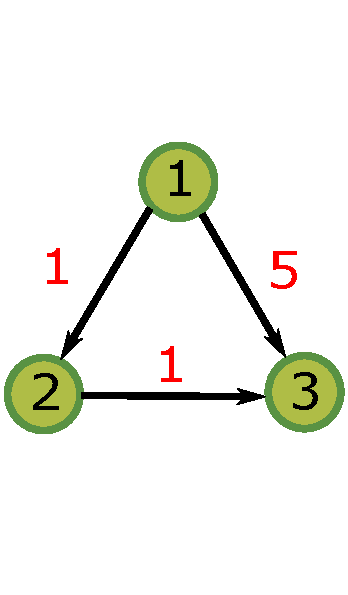
\includegraphics[width=\textwidth]{example_directed.pdf}
  \caption{一个有三个节点的带权有向图}
  \label{fig:example_directed}
  \end{subfigure}~
  \begin{subfigure}[b]{0.5\linewidth}
    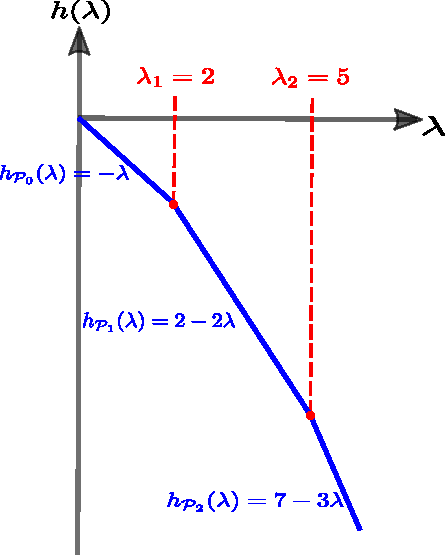
\includegraphics[width=\textwidth]{dt.pdf}
    \caption{$h(\lambda)$ 的图像}
    \label{fig:dt}
    \end{subfigure}  
    \caption{主划分序列求解示意图}
\end{figure}

因为
$G$ 包含的节点只有3个,可以使用枚举法计算对应的 $h(\lambda)$
函数,其函数图像如图 \ref{fig:dt} 所示。其中
$\P_0=\{ \{1,2,3\} \}, \P_1 = \{\{1,3\}, \{2\} \},
\P_2 =\{\{1\},\{2\},\{3\} \}$。
从图 \ref{fig:dt} 中可以看到,在这个简单的例子中
$h(\lambda)$
是一个分段线性函数。一般的图$G$对应的
$h(\lambda)$ 也是如此。

因此,基于图划分的方法,\ref{fig:example_directed}
中的图将被 划分成 $\P^*=\P_1$,即节点1和3被分成一类,
而节点2单独分成1类,这符合我们的直觉。

\newacronym{acr:psp}{PSP}{Principal sequence of partition}
\newglossaryentry{psp}{name=主划分序列, description={Principal sequence of partition}}
对于一般的图,其节点数目可能很多,此时用枚举法计算
$h(\lambda)$ 变得不可行。\citet{narayanan} 指出,计算
$h(\lambda)$ 有多项式时间的算法。因该算法是最早求解主划分序列 的算法,
我们把这一算法称为PSP算法。
由于原文献年代较为久远,作为替代,下面我们参考文献\inlinecite{mac}
对PSP算法进行简要介绍。
%\subsection{主划分序列}    

求解 \eqref{eq:PSP_structure} 只需得到在每一个
分界点处对应的 $\lambda$ 和 $\P$ 即可。
考虑到 $\P_k \preceq \dots \preceq \P_1 \preceq \P_0$
,
我们有 $|\P_0| \leq |\P_1| \dots \leq |\P_k|$,
即随着 $\lambda $ 的增大,线性函数斜率的绝对值逐渐增大。
这从图 \ref{fig:dt} 中也可以得到印证。
利用这一特点并基于分治的思想,算法 \ref{alg:psp} 
给出了获得主划分序列的步骤。

\renewcommand{\algorithmicrequire}{\textbf{输入:}\unskip}
\renewcommand{\algorithmicensure}{\textbf{输出:}\unskip}

\begin{algorithm}[!ht]
  \caption{求解主划分序列的算法 (PSP算法)}
  \label{alg:psp}
  \small
  \begin{algorithmic}[1]
    \REQUIRE 图$G$
    \ENSURE 序列 $L=[\lambda_1, \dots, \lambda_k]$
    和 $\mathcal{Q}=[\P_0, \dots, \P_k]$
    \STATE $L \leftarrow []$
    \STATE $\mathcal{Q}\leftarrow \{V\}, \P \leftarrow \{ \{i \} | i \in V\}$
    %\STATE $\mathbf{PSP}= [Q, P]$
    \STATE \texttt{Split}$(\mathcal{Q},\P)$
    \STATE 对 $L$ 和 $\mathcal{Q}$
    按从小到大排序 \footnotemark
    \FUNCTION{\texttt{Split}$(\mathcal{Q},\P)$}
     \STATE\label{alg:lambda} $\lambda' =
     {1 \over \abs{\P} - \abs{\mathcal{Q}}}
     (f(\P)-f(\mathcal{Q}))$
     \STATE\label{alg:lambda_plus} $h' = {1 \over \abs{\P} - \abs{\mathcal{Q}}} 
     (\abs{\P} f(\mathcal{Q}) - \abs{\mathcal{Q}} f(\P))$
     \STATE\label{alg:lambda_f} $(\tilde{h}, \P') = \texttt{DT}(G,\lambda')$
     \IF{$\tilde{h} = h'$}
       \STATE\label{algorithme:terminer} 将 $\lambda'$ 插入 $L$
     \ELSE
       \STATE 将 $P'$ 插入 $\mathcal{Q}$
       \STATE\label{algorithme:gauche} \texttt{Split}$(\mathcal{Q}, \P')$
       \STATE\label{algorithme:droit} \texttt{Split}$(\P',\P)$
     \ENDIF
    \ENDFUNCTION
  \end{algorithmic}
\end{algorithm}


在算法 \ref{alg:psp} 第 \ref{alg:lambda} 、 \ref{alg:lambda_plus} 行,
求解 $(\lambda', h')$ 相当于在二维 $(\lambda, h)$
平面上计算直线
$h = f[\P] - |\P| \lambda $
和 $h = f[\mathcal{Q}] - |\mathcal{Q}| \lambda $ 的交点。
假设 $\P, \mathcal{Q}$ 对应的
$h(\lambda)$函数的分界点分别是 $\lambda_{\P}, \lambda_{\mathcal{Q}}$
($\{V\}$ 对应 0,
$\{\{i\}|i\in V\}$ 对应 $+\infty$),那么根据几何直观
$\lambda_{\mathcal{Q}} \leq \lambda' \leq \lambda_{\P}$。
紧接着, \ref{algorithme:gauche} 行的调用对应在
$[\lambda_{\mathcal{Q}}, \lambda']$
区间范围内寻找剩余的分界点,而
 \ref{algorithme:droit} 行的调用对应在
$[\lambda', \lambda_{\P}]$
区间范围内寻找剩余的分界点。最后,
 \ref{algorithme:terminer} 行表明
$[\lambda_{\mathcal{Q}}, \lambda_{\P}]$ 内没有分界点,无需再调用
\texttt{Split} 函数。

\newglossaryentry{dt}{name=迪尔沃思截断, description={Dilworth truncation}}
在算法 \ref{alg:psp} 第 \ref{alg:lambda_f} 行,
函数 \texttt{DT} (Dilworth truncation)被用来求解式\eqref{eq:hlambda} 获得最优值
$\tilde{h}$ 和最优值对应的划分 $\P'$。\footnotetext{$\mathcal{Q}$
中按集合的大小排序}
%该函数 \texttt{DT}
%
%是用于求解式\eqref{eq:hlambda}的算法,它实际上是一种贪心算法,
%由算法 \ref{alg:dt}  给出。
% \begin{algorithm}
%   \caption{迪尔沃思截断算法}\label{alg:dt}
%   \begin{algorithmic}[1]
%   \REQUIRE 图 $G$ 和 $\lambda$
%   \ENSURE  $\P$ 和 $h$
%   \STATE
%   $V^0 = \emptyset, x $ 是 $n$ 长的向量\footnotemark,
%   $\mathcal{A} = \{\}$
%   \FOR{$l=1, 2, \dots, n$}
%   \STATE $V^l = \{l\} \cup V^{l-1}$
%   \STATE\label{alg:tight} 计算 $x^* = \displaystyle\min_{ A: l \in A \subseteq V^l} f(A)- x(A)$。
%    $T^l$ 是达到此最小值的集合,并且 $x_l \leftarrow x^* - \lambda$。 
%     \STATE $U^l = T^l \cup [\cup \{A | A \in \mathcal{A}, A \cap T^l \neq \emptyset\}] $
%   \STATE $\mathcal{A} = \{U^l\} \cup \{A | A \in \mathcal{A}, A \cap T^l = \emptyset \}$
%   \ENDFOR
%   \STATE $\P^* = \mathcal{A}, h_{\lambda} = x(V)$
%   \end{algorithmic}
%   \end{algorithm}
% \footnotetext{$n$ 是图$G$中节点的个数}
在该函数
% \ref{alg:dt} 
%涉及到一种新的运算记号$x(A)$,
%这里 $x$ 表示一个向量而 $A$ 是一个集合
%$x(A)$ 定义为 $\sum_{i \in A} x_i$。
%此外,采用\cite{chan2017pin}中的方法,我们可以把 \ref{alg:tight}  行中的最优化
中调用了
%问题转化成
求解有向图上的最大流问题的算法。
% 具体而言,
% 针对 $\displaystyle\min_{ A: l \in A \subseteq V^l} f(A)- x(A)$,
% 我们首先构造一个图$G'$包含节点$V'=\{0, 1, 2, \dots, l\}=\{0\} \cup V^l$。
% 节点 $0$ 是相对新加入的,作为最大流算法的源节点。
% 而$l$是目标节点。图$G'$中有向边的权值有如下定义:
% \begin{equation}\label{eq:wij_prime}
%   w'_{ij} = \begin{cases}
%     \max\{0, -x_{i}\} & \textrm{ if } i = 0 \\
%     \max\{0, -x_{i}\} + w_{il} & \textrm{ else if } j = l \\
%     w_{ij} & \textrm{ otherwise }
%   \end{cases}
% \end{equation}
%
% 按照定义式 \eqref{eq:wij_prime}, 源节点0和目标节点j
% 之间的权值为零,即两节点间没有边相连。
% 基于定义好的图$G'$和$s=0,t=l$,我们求解如下
% 标准的最小割问题:
% \begin{equation}\label{eq:mincut}
%   \beta = \min_{A \subseteq V^l: l\in A }
%   c(V' \backslash A, A)
% \end{equation}
%
% 达到式\eqref{eq:mincut}
% 最小值的集合即是 $T^l$,并且$x^*$和 $\beta$
% 有如下关系式:
% \begin{equation}\label{eq:beta_alpha}
%   \beta = x^* + \sum_{x_v > 0, 1\leq v < l} x_v
% \end{equation}
%
%
%\subsection{参数化的最大流算法}
%最大流算法用于解决网络流中从一点到另一点的最优运输路径的问题。
\newglossaryentry{pra}{name=推送重贴标签, description={Push–relabel}}

求解最大流问题
有一类基于推送重贴标签 (Push-relabel) 的算法\cite{Goldberg1988}
具有良好的效率。如果要解一系列的最大流问题并且这一系列的问题
之间有一定的关联性,重复调用最大流算法显然不是最优的选择。
基于这种考虑,有学者提出了参数化的最大流算法\cite{Gallo1989}用于求解
具有特殊结构的一系列的最大流问题。
%下面对参数化的最大流算法
%进行简单的介绍。
%
% 首先让我们回顾一下最大流问题。
% 考虑一有向图$G(V,E)$。其节点集$V$
% 中包含两个特殊的节点:源节点$s$
% 和目标节点$t$。对每一对有向边
% $(u,v)$存在一个非负的容量函数
% $c(u,v)$。如果$u,v$之间没有有向边
% 定义$c(u,v)=0$。
% 最大流问题是求解流量函数
% $f(u,v)$,使得$\sum_{v\in V} f(v,t)$
% 最大。流量函数需要满足如下约束
% \begin{align}
%   f(u, v) \leq c(u, v) \textrm{ for } (u, v) \in V \times V \\
%   f(u, v) = -f(v, u) \textrm{ for } (u, v) \in V \times V \\
%   \sum_{v \in V} f(u,v) = 0 \textrm{ for } v\in V\backslash\{s, t\}
% \end{align}
% 最大流和形如式\eqref{eq:mincut}所示的最小割问题
% 互为对偶问题。因此求解最大流问题的算法也可以
% 用于求解最小割问题。
%
% 参数化的最大流算法考虑的问题是在最大流问题的
% 基础上,假设$c(s,v)$ 
% 是关于$\lambda$的增函数
% 且$c(v, t)$是$\lambda$的减函数,
% 分别记为
% $c_{\lambda}(s,v)$ 和 $c_{\lambda}(v, t)$。
% 对于一系列的$\lambda_1 < \dots < \lambda_k$,
% 我们可以得到 $k$ 个最大流问题。
参数化的最大流算法
基于前置推送-标签重贴算法,通过保留
在$\lambda_{i-1}$上的计算状态并用于下一步的初始化,
以及适当地使用并行化的技术,使得计算$k$ 个最大流问题
的时间复杂度和只计算一个最大流问题近似相等。
\citet{kolmogorov} 基于参数化最大流,将求解式\eqref{eq:hlambda}
转化为求解$n$次参数最大流问题。该并行算法宣称可达到 $O(n^4)$ 的时间复杂度。


\section{随机块模型}\label{sec:sbm}
随机块模型是我们研究社团发现问题主要使用的概率统计模型,我们将在
本小节对其进行简要介绍。与之相关的,我们将介绍随机块模型的精确恢复问题,从而引出误差率的概念;
此外,我们将对随机块伊辛模型这一工作进行简要介绍,该工作构成了我们第 \ref{chap:sibm} 章研究的基础。
最后,我们还介绍了与我们研究有关的两个社团发现算法。

\subsection{随机块模型及其精确恢复问题}\label{sec:exact_recovery}
\newglossaryentry{sbm}{name=随机块模型, description={Stochastic block model}}
\newacronym{acr:sbm}{SBM}{Stochastic block model}
随机块模型(Stochastic block model, SBM)是社团发现问题中最常用的统计模型之一
\cite{holland1983stochastic, abbe2017community},
本节介绍我们研究的一类特殊的随机块模型,
%它提供了一个基准人工数据集来评估不同的社团检测算法
%并启发了许多社团检测任务算法的设计 \cite{fortunato2010community}。
%
为此我们首先定义一些常用的符号。随机图仍用符号$G$表示,
每个节点的标签为 $X_i$,
\newglossaryentry{not:W}
{
  type=notation,
  name={\ensuremath{W}},
  description={$k$阶循环群,即$\{1, \omega, \dots, \omega^{k-1}\}$}
}
从  $W= \{1, \omega, \dots, \omega^{k-1}\}$中取值。
为方便后续讨论,这里我们给$W$赋予群的结构,让它成为一个阶为$k$的循环群,
即$\omega^k=1$,比如复平面上的单位根即有这样的结构。
特别地,当$k=2$时,$W=\{\pm 1\}$。
\newglossaryentry{not:Wn}
{
  type=notation,
  name={\ensuremath{W^n}},
  description={集合$W$的$n$次笛卡尔积}
}
$W^n$ 表示集合$W$的$n$次笛卡尔积。 

\newacronym{acr:ssbm}{SSBM}{Symmetric stochastic block model}
下面给出有$k$个社团的对称的随机块模型
(Symmetric stochastic block model, SSBM)
的定义: 
	\begin{definition}[有$k$ 个社团的 SSBM]\label{def:SSBM}
	令 $0\leq q<p\leq 1$, $V=[n]$ 且
  $X=(X_1,\dots,X_n)\in W^n$。 对任意的 $u\in W$,
  $X$ 满足约束
  $|\{v \in [n] | X_v = u\}| = \frac{n}{k}$。
	如果下面两个条件满足,
  则称随机图 $G$ 是通过 $\SSBM(n,k,p,q)$ 模型产生的。 
	\begin{enumerate}
	\item 若 $X_i=X_j$, $G$ 在 节点 $i$ 和节点 $j$之间存在边的概率是 $p$; 
 若 $X_i \neq X_j$,  在 节点 $i$ 和节点 $j$之间存在边的概率是 $q$。
	\item 每条边的存在与否相互独立。
	\end{enumerate}
\end{definition}

在定义\ref{def:SSBM}中,注意到 $p>q$,
说明同一社团之间的节点有边相连的概率更大,而
属于不同社团的节点之间有边相连的概率较小。

\newglossaryentry{Bernoulli_distribution}{name=伯努利分布, description={Bernoulli distribution}}
为进一步解释随机块模型,
我们定义随机变量 $Z_{ij}:=\mathds{1} [(i,j) \in E(G)]$,
它是表示节点$i$和节点$j$之间是否存在边的指示函数。
给定节点的标签向量 $X$,$Z_{ij}$ 服从伯努利分布,
\newglossaryentry{not:expectation}
{
  type=notation,
  name={$\E[\cdot]$},
  description={数学期望}
}
\newglossaryentry{mle}
{name=最大似然估计,
description={Maximum likelihood estimation}}
其数学期望值为
\begin{equation}
\E[Z_{ij}] =
\begin{cases}
p & X_i = X_j \\ 
q & X_i \neq X_j
\end{cases}
\end{equation}
则 有 $n$ 个节点的随机图 $G$ 
被 
随机变量 $Z:=\{Z_{ij}\}_{1\leq i<j\leq n}$ 完全确定。
这里,每一个 $Z_{ij}$ 是相互独立的。
$Z$ 的分布函数可以写为:
\begin{align}
P_G(\bar{G}):=& P_G(Z = z| X=x) \notag\\
=& p^{\sum_{i,j=1}^n
z_{ij}\delta(x_i, x_j)}q^{\sum_{i,j=1}^n z_{ij}(1-\delta(x_i, x_j))} \notag\\
\quad& \cdot (1-p)^{\sum_{i,j=1}^n (1-z_{ij})\delta(x_i, x_j)}
(1-q)^{\sum_{i,j=1}^n (1-z_{ij})(1-\delta(x_i, x_j))}
\label{eq:GmL}
\end{align}
上式中$P_G$中的下标$G$表示图$G$是由SSBM模型随机生成的,而
$\bar{G}$是$G$的一个样本。
若 参数 $p, q$ 已知,
通过求
式\eqref{eq:GmL} 的最大值
我们可以获得节点标签的估计量$\hat{X}$,此即
利用最大似然估计做社团发现。
%\footnote{Maximum Likelihood, 缩写为 ML}。
\newglossaryentry{not:cGn}
{
  type=notation,
  name={$\cG_n$},
  description={所有包含$n$个节点的图的集合}
}

同时我们介绍一个后文中会用到的符号$\cG_n$,它表示
所有包含$n$个节点的图的集合。
由概率分布归一化的性质可得,
$P_G(\cG_n) = \sum_{\bar{G}\in \cG_n}P_G(\bar{G})=1$。
\newacronym{acr:ml}{ML}{Maximum likelihood}

不加说明的情况下,最大似然(Maximum likelihood, ML)估计算法 是无约束的。但在
定义\ref{def:SSBM}的假设下,
还有一个额外的约束,即 $X$ 中每一类的标签数量是严格相等的。
在这个约束下最大化式\eqref{eq:GmL} 我们可以得到一个等价
的优化问题——$k$类的最小割问题,
其形式为:
\begin{equation}\label{eq:minimum_k_cut}
  \min_{x\in W^n} \sum_{ (i,j) \in E} (1-\delta(x_i, x_j))
\end{equation}
这里,函数 $\delta(x,y)$ 定义为:
当 $x=y$ 时,$\delta(x,y) = 1$; 当 $x\neq y$,$\delta(x,y)=0$。
\newglossaryentry{not:deltaxy}
{
  type=notation,
  name={$\delta(x,y)$},
  description={当 $x=y$ 时,$\delta(x,y) = 1$; 当 $x\neq y$,$\delta(x,y)=0$}
}

\newglossaryentry{planted}{name=植入性划分模型, description={Planted partition model}}
当$k=2$时,式\eqref{eq:minimum_k_cut} 即为植入性划分模型,
是图论中经典的NP难的二分问题之一。


随机块模型的精确恢复是指某社团发现算法可正确恢复
由随机块模型生成的图的全部节点标签。
因为我们考虑的是随机图,精确恢复是一个概率事件,
当图的节点数目趋于无穷大时,
若该准确概率收敛到1,则我们称达到精确恢复的要求。
为给出精确恢复的数学定义,
需要引入如下置换的符号。

\newglossaryentry{not:dist}
{
  type=notation,
  name={$\Dist(\sigma, \sigma')$},
  description={两个$W^n$中的向量的汉明距离,即$|\{i\in[n]:\sigma_i\neq \sigma'_i\}|$}
}
我们用 $S_k$ 表示 $W$  上所有的置换函数的集合, 
$f$ 是 定义在 $W$ 上的置换函数
并且可以通过逐元素作用的方式
将其定义域扩展到 $W^n$ 上。
对于任意 $\sigma \in W^n$,
定义集合 $S_k(\sigma):=\{f(\sigma)| f\in S_k\}$。
此外,我们定义两个$W^n$中的向量的
距离为$\Dist(\sigma, \sigma')=|\{i\in[n] |\sigma_i\neq \sigma'_i\}|$,
其中 $\sigma,\sigma'\in W^n
$。
\begin{example}
当 $n=2$ 且 $k=2$ 时,
取$\sigma=(1, \omega) \in W^2$。
$\omega$满足
$\omega^0 = 1$ 且 $\omega \cdot \omega = \omega^2 = 1$。
令 $f$ 是一个$W$上映射,定义为
$f(1) = \omega$ 且 $f(\omega)=1$,
则 $f \in S_2$ 且 $f(\sigma) = (\omega, 1)$。
另外我们有 $\Dist(\sigma, f(\sigma)) = 2$,
$S_2(\sigma) = \{\sigma, f(\sigma)\}$, 且
$S_2^c(\sigma) = W^2 \backslash S_2(\sigma)
=\{(1, 1), (\omega, \omega)\}$。
\end{example}

给定 随机块模型,精确恢复问题的数学定义如下:
\newglossaryentry{exact_recovery}{name=精确恢复, description={Exact recovery}}
\begin{definition}[SBM 中的精确恢复] \label{def:SSBMR}
给定节点标签 $X$,
并假设随机图 $G$ 从 $\SSBM(n,k,p,q)$ 模型中采样。
一个社团发现算法$\hat{X}$ 已知 $G$ 去估计$X$,
也被称做$X$ 的估计量。我们称该算法
可精确恢复$X$,如果准确概率
$P_a(\hat{X}):=P(\hat{X} \in S_k(X)) $满足
\begin{equation}\label{eq:Pa_hat_X}
P_a(\hat{X})
\to 1 \textrm{ 当 }\, n \to \infty
\end{equation}
\end{definition}

在上述定义中,记号 $\hat{X} \in S_k(X)$ 表示
我们只能获得置换意义下相对于真实标签$X$的恢复结果。
这是因为没有一个类别的基准导致的。
这种情况在无监督学习领域比较常见。
%式\eqref{eq:Pa_hat_X}中记号 $P_a(\hat{X})$
%表示 估计量 $\hat{X}$ 的
%准确概率。
\begin{remark}\label{rem:metric_exact_recovery}\,
  \begin{enumerate}
    \item 令 $P_e(\hat{X}) = 1 - P_a(\hat{X})$
    表示错误概率。
    定义\ref{def:SSBMR}也可以写成当$n\to \infty$
    时,
    $P_e(\hat{X}) \to 0$。
  \item  %此外,我们要指出的是,对给定的图 $G$,估计量$\hat{X}$可以是确定性的也
  %可以是随机的。
  一般而言, $\hat{X} \in S_k(X)$ 发生的概率 应该理解
  对随机图的平均 $\sum_{\bar{G} \in \cG_n} P_G(\bar{G}) P_{\hat{X}|\bar{G}}(\hat{X} \in S_k(X))$。 
  如果$G$是非随机的图,这个概率是 $P_G(\hat{X} \in S_k(X))$。  
  \end{enumerate}
\end{remark}

%在定义\ref{def:SSBMR}中,精确恢复也称强恢复。强恢复是相对于弱恢复
%而言的,前者要求所有节点都要分对,而后者只要求分对节点的比率收敛到1即可。
%关于这两种恢复条件近年来涌现大量相关的研究工作,
%因为我们的工作只涉及强恢复,
基于定义\ref{def:SSBMR},
下面对一些和精确恢复有关的重要结论进行逐一介绍。

设$a>b>0$,针对两个社团($k=2$)且$p=\A,q=\B$的情形,
Abbe \cite{abbe2015exact} 和 Mossel
\cite{mossel2016} 分别独立地研究发现了最大似然算法
精确恢复误差的变化规律。
因为最大似然算法相当于理论最优的估计量,他们的成果可总结为如下定理:
\begin{theorem}\label{thm:sbm2_phase_transition}
设 $P_e=P(\hat{X} \neq \pm X)$, 当 $n \to \infty$,
对于 $\SSBM(n,2,\A, \B)$ 模型,
有如下两种情形:
	\begin{enumerate}
		\item $\sqrt{a} - \sqrt{b} > \sqrt{2}$时,
    $P_e \to 0$, 存在算法满足精确恢复的要求;
		\item $\sqrt{a} - \sqrt{b} < \sqrt{2}$时,
    $P_e \to 1$,没有算法可实现精确恢复。
	\end{enumerate}
\end{theorem}
定理 \ref{thm:sbm2_phase_transition} 揭示了
具有2个社团结构的随机块模型在精确恢复度量下的相变规律。
该结论很快被Abbe 推广到$k>2$的情形
\cite{abbe2015community},由
定理 \ref{thm:sbmk_phase_transition} 给出。
该结果可以视为一般的随机块模型
精确恢复条件的一个特例。

\begin{theorem}\label{thm:sbmk_phase_transition}
  对于 $\SSBM(n,k,\A, \B)$ 模型,当条件
  \begin{equation}\label{eq:abk}
    \sqrt{a} - \sqrt{b} > \sqrt{k}
  \end{equation}   
  满足时,
  精确恢复可实现,
  而当$\sqrt{a} - \sqrt{b} < \sqrt{k}$时,
  没有算法可实现精确恢复。
\end{theorem}
\newglossaryentry{hellinger}{name=海林格距离, description={Hellinger distance}}
\begin{remark}
  Abbe 在文章中指出,定理 \ref{thm:sbmk_phase_transition} 
  给出的结论和海林格距离 (Hellinger distance)有关。
  % 对于两个$\R^d$中的向量$u,v$,它们的
  % 海林格距离 
  % 的平方定义为
  % \begin{equation}
  %   H^2(u,v) = \frac{1}{2}
  %   \sum_{i=1}^d (\sqrt{u_i} - \sqrt{v_i})^2
  % \end{equation}
  % 若定义向量 $u= (\frac{a}{k}, \frac{b}{k})$,
  % $v =  (\frac{b}{k}, \frac{a}{k})$,。
  % 则
  % $\sqrt{a} - \sqrt{b} > \sqrt{k}$ 的条件
  % 可改写成
  % $H(u, v) > 1$,其中
  % \begin{equation}\label{eq:Hellinger_abuv}
  %   H(u,v)=\frac{\sqrt{a} - \sqrt{b}}{\sqrt{k}}    
  % \end{equation}
  % 上面介绍的是Abbe 引入的切尔诺夫-海林格距离的定义,
  但他在文章中使用的距离度量仅是一般的测度而不是概率测度,
  其解释略显生硬。
\end{remark}

\subsection{随机块-伊辛模型}\label{sec:ising}
\begin{figure}
	\centering
	\begin{subfigure}{0.5\textwidth}
    \centering
    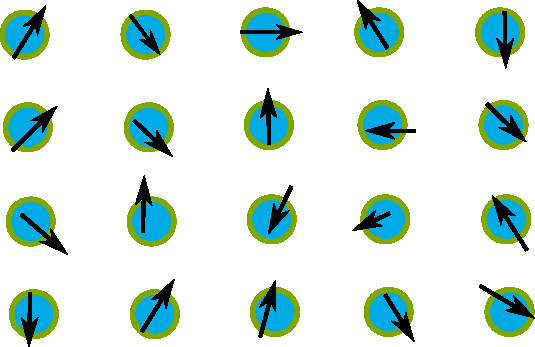
\includegraphics[width=0.7\textwidth]{Tlarge.pdf}
		\caption{$T>T_c$, 自旋方向随机}
	\end{subfigure}~
	\begin{subfigure}{0.5\textwidth}
    \centering
    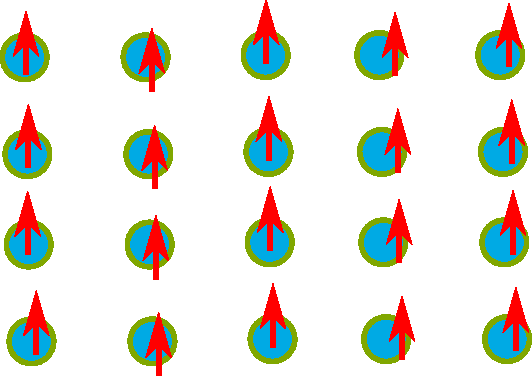
\includegraphics[width=0.7\textwidth]{Tsmall.pdf}
		\caption{$T<T_c$, 自旋方向一致}
	\end{subfigure}
  \caption{磁偶极矩自旋方向随温度变化示意图}\label{fig:ising_two_configurations}
\end{figure}   

在统计物理学中,伊辛模型指的是
可以处于两种自旋状态的磁偶极矩的集合\cite{ising1925beitrag}。
如图 \ref{fig:ising_two_configurations} 所示,
当外界温度$T$
大于临界温度 $T_c$ 时,
各磁偶极矩处于杂乱无章的状态,其总的磁化强度接近0。
但当外界温度$T$
小于临界温度 $T_c$ 时,
各磁偶极矩的状态则变得方向一致。
这里,我们称这种方向一致的现象叫自发磁化。


\begin{figure}
	\centering
	\begin{subfigure}{0.45\textwidth}
		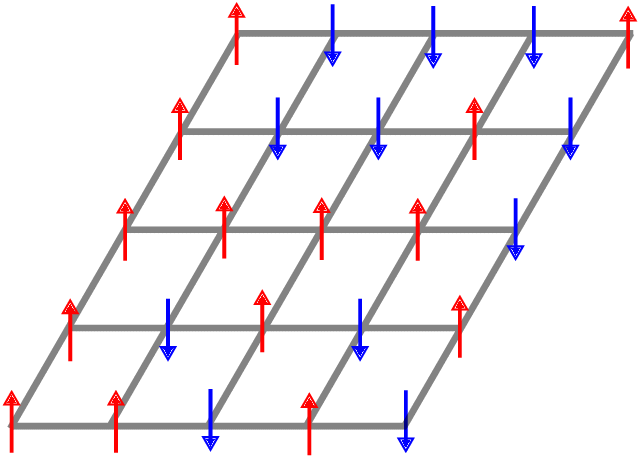
\includegraphics[width=\textwidth]{square-lattice.png}
		\caption{正方形网格}\label{fig:square_lattice}
	\end{subfigure}~
	\begin{subfigure}{0.53\textwidth}
		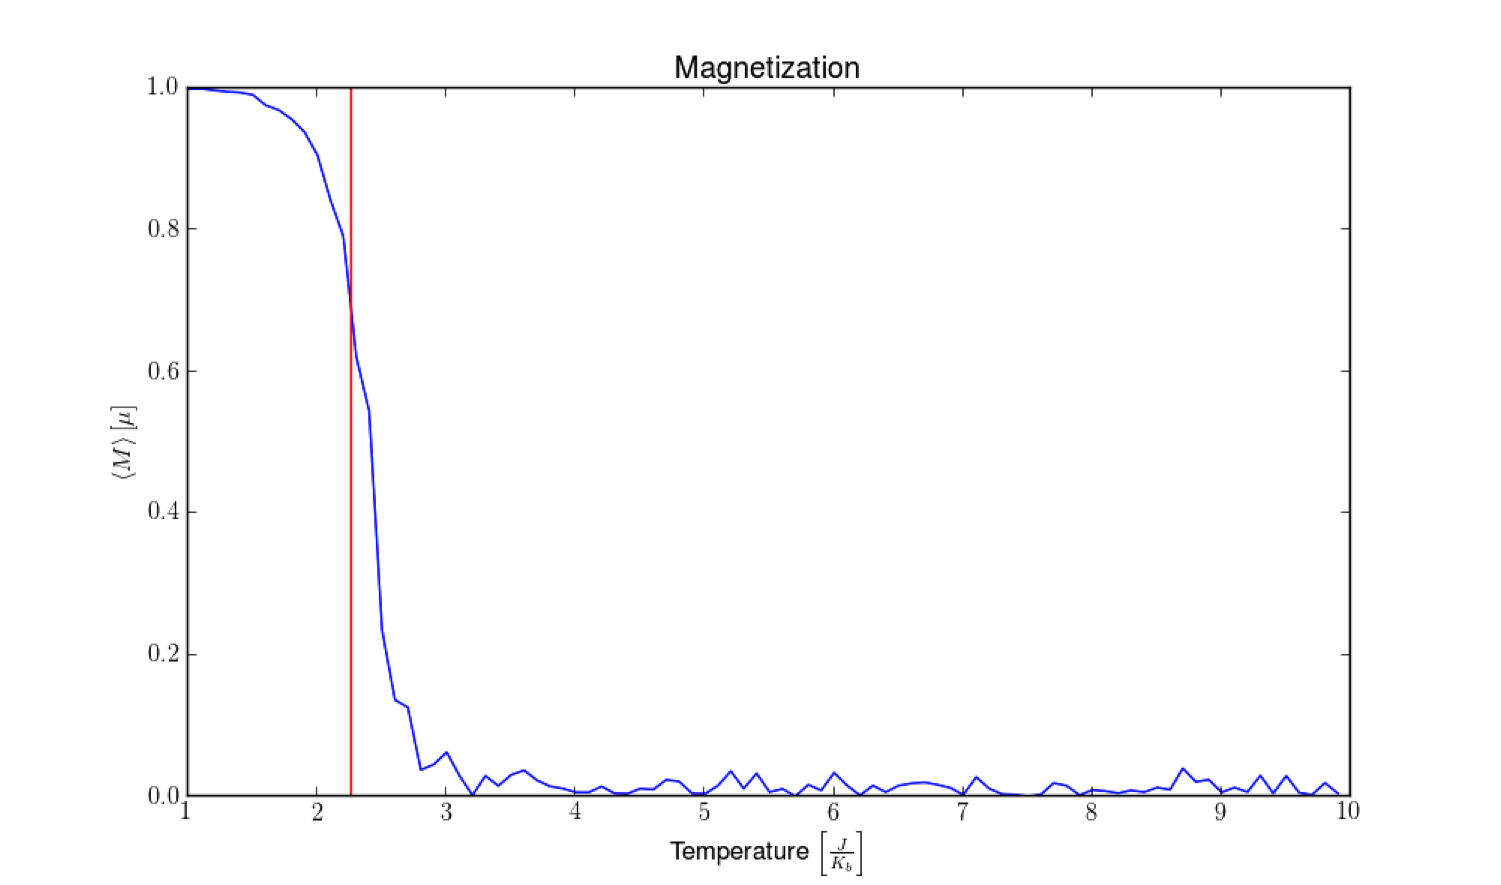
\includegraphics[width=\textwidth]{monte-carlo-ising-6.png}
		\caption{$M$随温度变化情况\footnotemark}\label{fig:square_lattice_b}
	\end{subfigure}
  \caption{正方形网络上的伊辛模型及其磁化强度的变化}
\end{figure}
\footnotetext{图源: http://www.bdhammel.com/ising-model/}
下面我们介绍伊辛模型中一些常用的概念,
如图 \ref{fig:square_lattice} 所示,
在一个正方形网格中的格点上分布着磁偶极矩,一共有$n$个。
$\sigma_i \in \{ \pm 1\} $ 表示第$i$个磁偶极矩的状态,
总的磁化强度为 $M = \frac{1}{n} \sum_{i=1}^n \sigma_i$。
理论研究时先考虑有限的正方形网格, 再取 $n\to \infty$。
由于磁偶极矩之间的磁力作用和受外场的影响,存在着磁化强度的相变现象,即
\begin{enumerate}
		\item $T< T_c, M>0$, 发生自发磁化。
		\item $T> T_c, M=0$, 无自发磁化。
\end{enumerate}

\newglossaryentry{phase_trans}{name=相变, description={Phase transition}}
图 \ref{fig:square_lattice_b} 中给出了自发磁化的仿真实验结果,其中临界温度用
红竖线标出。从图中可见在临界温度处磁化强度突然降为零,也即
磁偶极矩的自旋方向由完全一致变成两种状态各占一半。我们称临界温度处伊辛模型
的这种变化为相变(Phase transition)现象,
我们在第 \ref{chap:sibm} 章也将展示社团发现的精确恢复问题
中也有类似图 \ref{fig:square_lattice_b} 的相变现象。

\newglossaryentry{canonical}{name=正则系综, description={Canonical ensemble}}
对于自发磁化现象可以通过统计力学中的正则系综 (Canonical ensemble)
理论进行解释。该理论
假设粒子的分布为
\begin{equation}\label{eq:canonical_ensemble}
P(\sigma = \bar{\sigma}) = \frac{1}{Z} \exp(-\beta H(\bar{\sigma}))
\end{equation}
其中$\bar{\sigma} \in \{\pm 1\}^n$ 表示粒子的状态,
$H$叫做汉密尔顿能量函数,表示系统处于状态$\bar{\sigma}$时的总能量,$\beta$是与温度成反比的参数,
\newglossaryentry{inverse_temp}{name=逆温度, description={Thermodynamic beta}}
也叫逆温度(Thermodynamic beta),$Z$是配分函数,是概率分布的
归一化常数。


伊辛模型除了定义在正方形网格上外,还可以推广到一般的图 $G(V, E)$ 上。
对于没有外场的情形,伊辛模型的能量函数为
\begin{equation}\label{eq:hamiltonian}
	H(\sigma) = -\sum_{(i,j) \in E(G)} \sigma_i \cdot \sigma_j
\end{equation}
在微观层面上,每种微观状态出现的概率均正比于 $\exp(-\beta H(\bar{\sigma}))$,
概率越大或能量越低的状态越有可能出现;在宏观层面则表现为
磁化强度$M$的变化。

\begin{example}
  表 \ref{tab:particles_3} 给出了一个含有3个粒子的系统,其共有8种微观态,
  但根据式\eqref{eq:hamiltonian}, 其在宏观能量的表现了只有$H=-3$或 $H=1$两种组合。
\begin{table}
  \centering
\begin{tabular}{ccc}
		编号 & 微观态 & 宏观态 ($H$) \\
		1 & $\uparrow\uparrow\uparrow$ & -3 \\
		2 & $\uparrow\uparrow\downarrow$ & 1 \\
		3 & $\uparrow\downarrow\uparrow$ & 1 \\
		4 & $\downarrow\uparrow\uparrow$ & 1 \\
		5 & $\uparrow\downarrow\downarrow$ & 1    \\
6 & $\downarrow\uparrow\downarrow$ & 1 \\
7 & $\downarrow\downarrow\uparrow$ & 1 \\
8 & $\downarrow\downarrow\downarrow$ & -3 \\
\end{tabular}
\caption{一个含有3个粒子的系统的微观状态与宏观能量}
\label{tab:particles_3}
\end{table}
\end{example}

\newglossaryentry{not:all_one_vector}
{
  type=notation,
  name={\ensuremath{\mathbf{1}_n}},
  description={长度为 $n$ 的全1的向量}
}

将伊辛模型视为网络中一种刻画节点状态的概率模型,
有学者\cite{ye2020exact}
指出,式\eqref{eq:hamiltonian} 所描述的
伊辛模型不存在相变现象,因为式\eqref{eq:canonical_ensemble}
给出的分布聚集在 $\sigma=\pm \mathbf{1}_n$ 附近,
这里 $\mathbf{1}_n$ 表示长度为 $n$ 的全1的向量。
为此,可以采用下述修正模型,将没有边相连的粒子之间的
作用力考虑进来。
\begin{equation}\label{eq:ising_modified}
  H(\bar{\sigma}) = \gamma \frac{\log n}{n} \sum_{(i,j)\not\in E(G)}
  \bar{\sigma}_i \cdot \bar{\sigma}_j
	- \sum_{(i,j)\in E(G)}
  \bar{\sigma}_i  \cdot \bar{\sigma}_j
\end{equation}
这里引入了一个新的参数 $\gamma > 0$,表示反作用力的系数。
\eqref{eq:ising_modified}
相比于\eqref{eq:hamiltonian}
多了反作用力的项,在物理中类似自旋玻璃的模型\cite{lenka2016physics}。
因为该工作研究的是
由随机块模型 $\SSBM(n,2,p,q)$产生的图上定义的伊辛模型,
式\eqref{eq:ising_modified} 出现的系数
$\frac{\log n}{n}$
主要是为了与其研究场景 $p,q=O\left(\frac{\log n}{n} \right)$
相对应。

\newglossaryentry{metropolis}{name=梅特罗波利斯算法, description={Metropolis algorithm}}

梅特罗波利斯(Metropolis)算法\cite{metropolis1953equation}
被用于产生伊辛模型的样本。此外,该算法的变体“模拟退火”
\cite{pincus1970monte} 也是优化领域常用的随机算法。
其算法从系统一个随机的状态出发每次改变其中一个粒子
的状态并按一定的概率接受改变或保持原来的状态。
给定形如式\eqref{eq:ising_modified}
的能量函数,算法\ref{alg:Metropolis}
给出了梅特罗波利斯算法的步骤。

\begin{algorithm}
  \caption{梅特罗波利斯算法}\label{alg:Metropolis}
  \begin{algorithmic}[1]
    \STATE 随机初始化 $\bar{\sigma}$
    \STATE 随机选一个粒子进行状态翻转,新的系统状态记为 $\bar{\sigma}'$ 
    \STATE 计算能量差 $\upDelta H= H(\bar{\sigma}') - H(\bar{\sigma})$
    \IF{$\upDelta H < 0$}
    \STATE $\bar{\sigma} \leftarrow \bar{\sigma}'$
    \ELSE
    \STATE 以概率 $\exp(-\beta \upDelta H)$ 
    使得 $\bar{\sigma} \leftarrow \bar{\sigma}'$,
    否则保持原状。 
    \ENDIF
    \STATE 重复步骤 2-8 直到收敛。
\end{algorithmic}  
\end{algorithm}

\newglossaryentry{potts_model}{name=玻茨模型, description={Potts model}}

以上讨论的伊辛模型中粒子均只有$\{\pm 1\}$两个状态。
实际上每个粒子的状态数可以扩展到多个,即 玻茨模型\cite{potts1952some}。
类似式\eqref{eq:hamiltonian},标准玻茨模型的汉密尔顿能量公式为:
\begin{equation}\label{eq:Hsigma_multiple_state}
  H(\sigma) = -\sum_{(i,j) \in E(G)}\delta(\sigma_i, \sigma_j)
\end{equation}
\begin{remark}\label{rem:equivalence_H_energy}
需要注意的是,在状态数$k=2$的情形,
式\eqref{eq:Hsigma_multiple_state} 
与式\eqref{eq:hamiltonian}
并不严格等价。
从关系式$\delta(\sigma_i, \sigma_j) = \frac{\sigma_i \sigma_j + 1}{2}$
可以看出,它们之间差了一个伸缩变换。
\end{remark}

\newglossaryentry{sibm}{name=随机块-伊辛模型, description={Stochastic Ising block model}}
\newacronym{acr:sibm}{SIBM}{Stochastic Ising block model}
将 \ref{sec:exact_recovery} 小节 介绍的随机块模型与 本小节介绍的 伊辛模型
复合起来可得到随机块-伊辛模型(Stochastic Ising block model, SIBM)\cite{ye2020exact}。
该模型首先由 随机块模型生成随机图,
再由随机图上定义的 伊辛模型多次生成节点的状态。
SIBM 模型的恢复任务是由多次生成的节点状态估计节点的真实状态。
该复合模型可用于模拟两党制国家政治选举前的多次民意调查,
生成随机图依据的节点真实状态即为选民
的政治倾向。下面对SIBM的研究结果进行简要介绍。

在\citet{ye2020exact} 的研究工作中,由 $\SSBM(n,2,\A, \B)$
生成随机图,采用 \eqref{eq:ising_modified} 定义的能量函数
独立生成 伊辛模型的样本 $m$ 次,主要研究了样本复杂度$m$
的相变现象以及当$m=1$时参数$\beta$的相变现象。
这里的相变现象是针对SBM模型的精确恢复问题而言的,
即对于某一参数存在一个精确恢复能否实现的临界值点。

\citet{ye2020exact} 的工作中关注的重点是对采样数量$m$的相变现象的讨论,
而我们将在其工作的基础上,将伊辛模型拓展为节点有多个状态的玻茨模型,
重点研究$m=1$时参数$\beta$的相变现象以及相关的社团发现算法。

\citet{ye2020exact} 在其工作的技术证明中,用到了马尔可夫不等式和切尔诺夫不等式这两个概率论中常用的集中不等式。
由于我们在后面章节的技术证明中也要用到这两个不等式,故在本小节最后列出它们,方便后面引用。

\newglossaryentry{markov_ieq}{name=马尔可夫不等式, description={Markov's inequality}}
\begin{lemma}[马尔可夫不等式] 
  设 $X$ 是非负型随机变量,则对于非负实数$a$有
  \begin{equation}
    P(X\geq a) \leq {1 \over a} \E[X]   
  \end{equation}
   若$X$ 不一定非负,$a$ 是任意实数,可先取$e$指数再运用马尔可夫不等式,
   即有
   \begin{equation}\label{eq:chernoff_bound}
    P(X\geq a) = P(e^{tX} \geq e^{ta}) \leq { 1 \over \exp(ta)} \E[\exp(tX)]
   \end{equation}
   对任意的$t>0$成立。
   \newglossaryentry{chernoff}{name=切尔诺夫不等式, description={Chernoff inequality}}

   式\eqref{eq:chernoff_bound}也被称为切尔诺夫不等式。
\end{lemma}
\newglossaryentry{chebyshev_ieq}{name=切比雪夫不等式, 
description={Chebyshev's inequality}}
\begin{lemma}[切比雪夫不等式]
  \newglossaryentry{not:variance}
{
  type=notation,
  name={$\Var[\cdot]$},
  description={方差}
}
  对于随机变量 $X$, 正实数$a$,我们有
  \begin{equation}
    P(\abs{X-\E[X]} \geq a) \leq {1 \over a^2} \Var[X]
  \end{equation}
  这里,$\Var[X]$表示随机变量$X$的方差。
\end{lemma}

% to do: add large deviation theory and hypothesis testing


\subsection{最大模块度算法}

最后,我们再简单介绍一下社团发现领域常用的最大模块度算法
\cite{newman2006modularity}。
\newglossaryentry{modularity}{name=模块度, description={Modularity}}
模块度
是对网络中社团结构强弱程度的一种度量,既能作为评价
不同社团发现算法的性能指标,也能
通过近似求解其最大值的思路启发算法设计。
模块度越高,则社团内部连接越紧密,
而社团之间连接越稀疏。

给定长度为$n$的向量$x$,模块度的数学定义为:
\begin{align}\label{eq:Q}
  Q(x) &= \frac{1}{2 |E|} \sum_{ij} 
  \left(A_{ij} - \frac{d_i d_j}{2 |E|} \right) \delta(x_i, x_j)
\end{align}
这里 $A$ 表示图的邻接矩阵,$|E|$表示边的数量,
而$d_i$表示第
\newglossaryentry{degree}{name=度, description={Degree}}
$i$个节点的度(Degree),$x_i$ 表示第$i$
个节点所属的社团。

贪心法是用于近似求解式\eqref{eq:Q}
最大值的常用算法,其流程类似于系统聚类法,
即从每个节点各自属于一类出发,通过中间指标最大的方法每次聚合两类,
使得 $Q$ 不断增大。该思路可经过优化适用于求解大规模网络中
的社团发现问题 \cite{clauset2004finding}。

\subsection{基于半正定规划的社团发现算法}
\newacronym{acr:sdp}{SDP}{Semi-definite programming}
\newglossaryentry{sdp}{name=半正定规划, description={Semi-definite programming}}

针对随机块模型的社团发现
可以先将最大似然方法获得的目标函数
写成整数优化问题的形式,
再转化成半正定规划(Semi-definite programming, SDP) 的优化问题进行求解。

在 式\eqref{eq:minimum_k_cut} 中
取 $\delta(x_i, x_j) = \frac{1+x_ix_j}{2}$,
于是可得到如下
的优化问题:
\begin{align}
  \max_x\  &  x^{\mathrm{T}} A x \notag \\
  \textrm{s.t. } & x_{i} \in \{\pm 1\}, i \in [n] \notag \\
  & \mathbf{1}_n^{\mathrm{T}} x = 0
\end{align}
其中 $A$ 表示图的邻接矩阵。
$ x^{\mathrm{T}} A x $ 可以看成是 $\langle xx^{\mathrm{T}}, A \rangle $,即矩阵
\newglossaryentry{not:matrix_inner_product}
{
  type=notation,
  name={$\langle A, B \rangle $},
  description={矩阵$A$ 和 $B$ 的 Frobenius 内积}
}
\newglossaryentry{not:matrix_all_one}
{
  type=notation,
  name={$J_n$},
  description={元素全为1的$n\times n$的矩阵}
}
$xx^{\mathrm{T}}$ 与 $A$ 的内积。令$Y=xx^{\mathrm{T}}$,则$Y$是一个
半正定的矩阵,若对$Y$秩为1的条件进行松弛,则
得到如下半正定规划问题:
\begin{align}\label{eq:opt_A_Y_1}
  \max_Y\  & \langle A, Y \rangle  \notag \\
  \textrm{s.t. } & Y_{ii} = 1, i \in [n] \notag \\
  & \langle Y, J_n \rangle  = 0
\end{align}
其中 $J_n=\mathbf{1}_n\mathbf{1}_n^{\mathrm{T}}$
是元素全为1的$n\times n$的矩阵。
令 $R=2A + I_n - J_n$,
\newglossaryentry{not:identity_matrix}
{
  type=notation,
  name={$I_n$},
  description={$n\times n$的单位矩阵}
}
$I_n$ 是$n\times n$的单位矩阵,
则
优化的目标函数还可写成 $ \langle R, Y \rangle $,
其中 $R$ 可进一步写成
\begin{equation}\label{eq:def_B_sdp}
    R_{ij} = \begin{cases}
        1, & \text{若 $i$ 与 $j$ 有边相连}, \\
        -1,& \text{其他情况}
    \end{cases}
\end{equation}  

以上方法可针对一般的图$G$进行求解,
但对于$\SSBM(n,2, \A, \B)$,
Hajek 等学者 \cite{hajek2016achieving} 得到了SDP在随机块模型中精确恢复的
理论保证。
\begin{theorem}
  设 $\hat{Y}_n$ 是
  优化问题 \eqref{eq:opt_A_Y_1} 的解,$\sigma$ 是节点的真实标签向量。
  若 $\sqrt{a} - \sqrt{b}
  > \sqrt{2}$,
  则
  $\lim_{n\to\infty} P(\hat{Y}_n=\sigma\sigma^{\mathrm{T}})=1$。
\end{theorem}
\section{信息论度量}
由于本文要用到多种信息论度量研究
社团发现问题,下面依次对多变量互信息、速率函数、雷尼散度等相关知识进行简要介绍。
另外,由于我们在用多变量互信息研究社团发现算法过程中还用到了局部信息几何相关的知识,
本节也对局部信息几何做一个简要的介绍。
\subsection{多变量互信息}\label{sec:info_clustering}
\newglossaryentry{not:kl_dev}
{
  type=notation,
  name={$D(P_X||P_Y)$},
  description={分布$P_X$ 和 $P_Y$之间的 K-L 散度}
}
\newglossaryentry{mmi}{name=多变量互信息, description={Multivariate mutual information}}
\newglossaryentry{gmc}{name=广义最大相关, description={Generalized maximal correlation}}
\newacronym{acr:mmi}{MMI}{Multivariate mutual information}

在信息论领域,互信息提供了两个随机变量之间的
距离度量。使用 K-L 散度的记号,随机变量$X$
和 $Y$ 之间的互信息定义为:
\begin{equation}\label{eq:mutual_info}
  I(X;Y) = D(P_{XY} ||P_XP_Y)
\end{equation}
其中$P_X, P_Y$表示$(X,Y)$的边缘分布,$D(P_X||P_Y)$
表示分布$P_X$ 和 $P_Y$之间的 K-L 散度。
而$P_{XY}$
表示两个随机变量的联合分布。有多种方法可将互信息
的概念推广到两个及两个以上的随机变量间,
其中Chan等\cite{ska} 提出的一种推广 具有多种好的性质,
且涵盖了图结构的情形。我们把他的推广叫做多变量互信息 (Multivariate mutual information, MMI)。
这里我们需要指出,MMI 并不是多个随机变量之间信息量的唯一度量方法,
比如有学者基于HGR最大相关提出了广义最大相关 (Generalized maximal correlation)
也能实现类似的目的 \cite{huang2020information}。

下面我们对MMI做简要的介绍。令$V=[n]$是$n$个随机变量
序号的集合,$C$是 $V$的子集,$Z_C=\{Z_i | i \in C\}$
表示随机变量序号在 $C$ 中的随机变量 $Z_i$ 的集合。
$P_{Z_C}$表示$Z_C$的联合分布。
$\P, \Pi'$等符号在 \ref{sec:graph_strength} 节定义。
则MMI度量的定义为:
\begin{align}
  I(Z_V) &:= \min_{\P \in \Pi'} I_{\P}(Z_V)
  \label{eq:IZV}\\  
  \textrm{ 其中 } I_{\P}(Z_V) &:= \frac{1}{|\P| - 1}
  D\left(P_{Z_V} \Big|\Big| \prod_{C\in \P} P_{Z_C} \right) \label{eq:IPZV}
\end{align}
在上面的定义中,如果$Z_V$彼此独立,那么$I(Z_V)=0$,
反之亦然。

式\eqref{eq:IPZV}给出了特定划分下的多变量互信息,
也可根据下式把K-L散度改写成熵的形式。
\begin{equation}\label{eq:entropy_expression}
  D\left(P_{Z_V} \Big|\Big| \prod_{C\in \P} P_{Z_C} \right)
  = \sum_{C \in \P}
  H(Z_C) - H(Z_V)
\end{equation}
\newacronym{acr:pin}{PIN}{Pairwise independent network}

但对于一般的分布,式\eqref{eq:IZV}
难于计算。\citet{chan2017pin} 又提出了一种特殊的互独立网络 (Pairwise independent network, PIN) 模型,
使得多变量互信息可以用 \ref{sec:community_detection} 节
介绍的PSP算法进行计算。
这里略去PIN模型的数学定义,而是通过下面的例子
阐发它和图结构的联系。
\begin{example}\label{ex:mmi}
  令$V=\{1,2,3\}$,$Z_1=(X_a, X_c)$,
  $Z_2=(X_a,X_b)$ 且 $Z_3=(X_b,X_c)$。
  $X_a,X_b,X_c$是独立的随机变量且它们的熵分别为:
  $\mathcal{H}(X_a)=\mathcal{H}(X_b)=1, \mathcal{H}(X_c)=5$。
  利用联合熵的公式不难计算出$ \mathcal{H}(Z_1)=\mathcal{H}(X_a)+\mathcal{H}(X_c)$以及
  $\mathcal{H}(Z_1, Z_2) = \mathcal{H}(X_a) + \mathcal{H}(X_b) + \mathcal{H}(X_c)$等。
  若 $\P=\{\{1,2\}, \{3\}\}$,则根据
  \eqref{eq:entropy_expression}式,
  $D(P_{Z_V}||P_{Z_1,Z_2}P_{Z_3}) = \mathcal{H}(X_a)
  +\mathcal{H}(X_b)$。我们可以将上面的计算用图 \ref{fig:example_directed} 
  进行对应,即把$Z_i$对应到第$i$个节点,
  $Z_i$与$Z_j$之间的互信息对应到第$i$和第$j$个节点之间
  边的权值,而K-L散度即为不同的类别之间边的权值之和。
\end{example}
例 \ref{ex:mmi} 中虽然只有三个节点,
但对于一般的情形,PIN模型也和一个有向图有
着类似的对应关系。因此,在PIN模型下多变量互信息可以用
PSP算法进行计算。

基于多变量互信息可以对随机变量进行聚类,所有簇的集合
定义为
\begin{align}
  \mathcal{C}(Z_V) &:= \bigcup_{\gamma \in \R} \mathcal{C}_{\gamma}(Z_V)
  \label{eq:czv}\\
  \textrm{其中 } \mathcal{C}_{\gamma}(Z_V) &:= \textrm{maximal}
  \{ C \subseteq V \big\vert |C|>1, I(Z_C) > \gamma  \} 
\end{align}
上式中 maximal 表示在包含关系下最大的集合。
理论分析表明,基于定义式\eqref{eq:czv} 可以得到和
式\eqref{eq:PSP_structure}类似的层次聚类结果。
即存在一系列的临界值$\lambda_1 < \dots < \lambda_k$和划分
$\P_k \preceq \dots \preceq \P_0$,使得
$\mathcal{C}(Z_V) = \bigcup_{i=1}^{k} \mathcal{C}_{\lambda_i}(Z_V)$
且$\mathcal{C}_{\lambda_i}(Z_V) = \P_i$。

最后,我们再介绍一个多变量互信息的性质,它在我们后面研究异常值检测问题中
用到。这个性质给出了最大的临界值 $\lambda_k$
的多变量互信息的表达式\cite{agg_ic}:
\begin{equation}\label{eq:largest_threshold}
\lambda_k = \max_{C\subseteq V} I(Z_C)
\end{equation}

\subsection{局部信息几何}\label{sec:local_geometry}
局部信息几何\cite{huang2019universal}
可用于从理论层面上分析机器学习中的特征提取\cite{huang2017information}、人工神经网络
\cite{huang2019information}等问题。
下面对本工作中用到的局部信息几何的内容进行简要的介绍。

\newglossaryentry{pmf}{name=概率质量函数, description={Probability mass function}}

K-L散度可用于度量两种不同概率分布
之间的距离。当这两种分布比较接近时,
局部信息几何刻画了K-L散度的近似表达式。
我们以离散分布为例,给出表示分布之间距离接近的
形式化定义。
$P_0$ 表示一概率质量函数 (Probability mass function),
其定义域为有限的字母集$\mathcal{X}$,
$\epsilon$表示一无穷小量。
\begin{definition}\label{def:eps_neighborhood}
如果
\begin{equation}\label{eq:P_neighborhood}
\sum_{x \in \mathcal{X}} \frac{(P(x) - P_0(x))^2}{P_0(x)} \leq \epsilon^2
\end{equation}
\end{definition}
则我们称 $P$ 在 $P_0$的 $\epsilon$ 邻域 $\mathscr{N}^{\epsilon}(P_0)$ 内,记作$P \in \mathscr{N}^{\epsilon}(P_0)$。
式\eqref{eq:P_neighborhood}可以写成 $P(x) = P_0(x) + \epsilon
\sqrt{P_0(x)} \phi(x) + o(\epsilon)$的简化形式,其中 $\phi(x)$
叫做信息向量(Information vector),它的欧氏范数 $||\phi || $ 不超过1。
对于两个在$P_0$的$\epsilon$邻域内的分布 $P_1, P_2$,
记它们对应的信息向量分别为$\phi_1, \phi_2$,
则我们有
\begin{equation}\label{eq:approx:ig}
D(P_1 || P_2) = \frac{\epsilon^2}{2} ||\phi_1 - \phi_2||^2 + o(\epsilon^2)
\end{equation}
对于两个弱独立的随机变量,也有类似式\eqref{eq:approx:ig}
的结论。
\begin{definition}\label{def:weak_indepedent}
我们称 $X$ 和 $Y$ 是 $\epsilon$-弱独立的,
如果 对于任何 $x \in \mathcal{X}$,
$Y$关于$X$的条件分布
$P_{Y|X}(\cdot |x)$在$Y$的$\epsilon$邻域内。
\end{definition}
在弱独立的假设下,由 $D(P_{XY}||P_XP_Y)$ 所定义的互信息$I(X;Y)$, 
通过对式\eqref{eq:approx:ig}的化简,可以表示为:
\begin{equation}\label{eq:Ixy}
I(X;Y) = \frac{1}{2}\sum_{x\in \mathcal{X}, y\in \mathcal{Y}} B^2(x,y) + o(\epsilon^2),
\textrm{ 其中 }  B(x,y)=\frac{P_{X,Y}(x,y) - P_X(x) P_Y(y)}{\sqrt{P_X(x)P_Y(y)}}
\end{equation}
在式\eqref{eq:Ixy}中, $\sum_{x\in \mathcal{X}, y\in \mathcal{Y}} B^2(x,y)$
一项可以写成 $\norm{B}_{\mathrm{F}}^2$。这里 $B$表示$|\mathcal{X}| \times |\mathcal{Y}|$
的矩阵,称为典型相关矩阵(Canonical Dependence Matrix)\cite{huang2019universal},
\newglossaryentry{not:norm_f}
{
  type=notation,
  name={$||\cdot||_{\mathrm{F}}$},
  description={矩阵的Frobenius范数}
}
F 表示矩阵的Frobenius范数。
式 \eqref{eq:Ixy} 表明,当$X$和$Y$弱独立时有
\begin{equation}\label{eq:Ixy_B_F}
  I(X;Y)=\frac{1}{2} \norm{B}_{\mathrm{F}}^2
  +o(\epsilon^2)    
\end{equation}


\begin{example}\label{ex:Pweak_1}
设 $(X_0,Y_0)$是一个两维的随机向量,分布函数为$P_0$,
对于$x,y \in \{0,1\}$,
$P_0(x,y)=\frac{1}{4}$。
不难看出$X_0,Y_0$
是独立同分布的伯努利随机变量。
定义 $P(x,y)=\frac{1}{4}(1+\epsilon (-1)^{x+y})$,
则 $P\in \mathscr{N}^{\epsilon}(P_0)$,而
$\phi(x,y) = \frac{(-1)^{x+y}}{2}$
且有 $||\phi||=1$。
利用 $\log(1+x) = x - \frac{1}{2}x^2 + o(x^2)$
不难得到 $D(P_0||P)=\frac{\epsilon^2}{2}
+o(\epsilon^2)$,从而印证了
式\eqref{eq:approx:ig}的结论。
此外,根据定义 \ref{def:weak_indepedent} 
我们可以验证$X$与$Y$是弱独立的。
这里,$X\times Y$ 的分布函数是 $\frac{1}{4}(1+\epsilon (-1)^{x+y})$。
由式\eqref{eq:Ixy}可计算出
$I(X;Y)=\frac{1}{2}\epsilon^2+o(\epsilon^2)$,
与从互信息的定义式出发计算得到的结果相同,
从而印证
了弱独立情形下互信息的表达式。
\end{example}

\subsection{速率函数与大偏差原理}
本小节将首先从型的概念出发,引出针对离散随机变量的大偏差原理——Sanov定理。
型的概念和Sanov定理将在我们推导拓展随机块模型的最优误差率的结论中用到。
之后我们会
介绍大偏差原理的一般形式,即Cramér定理,从而引出速率函数的概念。

\newglossaryentry{type}{name=型, description={Type}}
在信息论中,我们首先假定所有的元素均从字母集$\mathcal{X}$
中选取。
某个长度为$n$的序列$x$的型是表示
其各字符在该序列中出现的比例,用符号$\hat{P}_x$表示,
而所有的$\hat{P}_x$组成集合$\mathbb{P}_n$。比如考虑字母集
$\mathcal{X}=\{1,2,3\}$,对于$11321$这个序列
它的型可以用三元组 $(\frac{3}{5}, 
\frac{1}{5}, \frac{1}{5})$ 表示。注意到
一个型对应着一个离散分布的概率质量函数。

假设 长度为$n$的序列$x=(x_1,\dots, x_n)$中每个元素 都是从分布 $Q(x)$
中独立采样,
则它的联合分布的概率质量函数可以记为$Q^n(x)=\prod_{i=1}^n Q(x_i)$。
对于任意长度为$n$的序列$x$,我们仍沿用上述关于$Q(x)$的定义。
为衡量$Q$和另一个不包括$Q$的概率分布的集合 $E$ 之间的距离,我们引入如下的记号:
$Q^n(E) = \sum_{x: \hat{P}_x \in E \cap \mathbb{P}_n} Q^n(x)$。
这里 $\hat{P}_x$ 是 $x$的型。

\newacronym{acr:iid}{i.i.d.}{Independent and identically distributed}

下面介绍的 Sanov 定理给出了$Q^n(E)$的上下界:
\begin{theorem}
  设 $X_1, \dots, X_n$ \glsname{acr:iid} 服从分布 $Q(x)$,
  若 $E$ 表示概率分布的集合,且$E$的闭包是其自身。
  则
  \begin{equation}
  \frac{1}{(n+1)^{|\mathcal{X}|}} e^{-n D(P^*||Q)}
  \leq Q^n(E) \leq (n+1)^{|\mathcal{X}|} e^{-n D(P^*||Q)}
  \end{equation}
  其中
  \begin{equation}
    P^* = \argmin_{P\in E} D(P||Q)
  \end{equation}
  极限情形下有:
  \begin{equation}\label{eq:limit_sanov}
    \lim_{n\to \infty} \frac{1}{n} \log Q^n(E) = -D(P^*||Q)
  \end{equation}
\end{theorem}
\begin{example}\label{ex:sanov_ldp}
若$X_1, \dots, X_n$ i.i.d. $\sim \Bern(p)$,
对于任意正数$\epsilon$,
我们可以用 Sanov 定理估计 $P\left(
  \frac{1}{n} \sum_{i=1}^n X_i > \E[X_1] + \epsilon
  \right)$ 随着$n$增大收敛到零
的速率。
此时集合$E=\{\Bern(q)| q>p+\epsilon\}$,
而$Q^n(E)=
P\left(\frac{1}{n} \sum_{i=1}^n X_i > \E[X_1] + \epsilon \right)$。
因此由式\eqref{eq:limit_sanov}可得
$\lim_{n\to \infty} \frac{1}{n} \log Q^n(E)=-D(\Bern(p+\epsilon)||\Bern(p))$。
\end{example}
Sanov 定理仅针对离散型分布给出了计算诸如
$P\left(\frac{1}{n} \sum_{i=1}^n X_i > \bar{X} + \epsilon \right)$
的方法,若将例 \ref{ex:sanov_ldp} 中诸$X_i$ 改为高斯分布,
则可以用Sanov 定理的推广形式 Cramér定理来解决。我们下面先介绍该定理:

\begin{theorem}\label{thm:cramer}
  \newglossaryentry{log_mgf}{name=对数矩生成函数, description={Logarithmic moment generating function}}
  \newacronym{acr:log_mgf}{log-MGF}{Logarithmic moment generating function}
  令 $X_1, \dots, X_n$ 为 i.i.d. 的随机变量序列,且$X_1$ 存在对数矩生成函数 (logarithmic moment generating function, log-MGF)
$\Lambda(t)=\log \E[\exp(t X_1)]$。
令 $\Lambda^*(s)= \sup_{t \in \R} (st-\Lambda(t))$,则对于所有$s>\E[X_1]$,
我们有
\begin{equation}\label{eq:cramer}
\lim_{n\to \infty} \frac{1}{n}\log P\left(
  \sum_{i=1}^n X_i \geq  ns \right) = - \Lambda^*(s)
\end{equation}
\end{theorem}
由于$\Lambda^*(s)$描述了$P( \sum_{i=1}^n X_i \geq  ns)$随$n$增大衰减到零的速率,
\newglossaryentry{rate_function}{name=速率函数, description={Rate function}}
我们把$\Lambda^*(s)$叫做速率函数。

为方便描述$\Lambda^*(s)$和$\Lambda(s)$的关系,
我们引入凸共轭函数的概念。
\begin{definition}\label{def:convex_conjugate}
  对于 $\R$ 上的光滑函数 $\Lambda(s)$,
  它的凸共轭函数定义为
  $\Lambda^*(s) = \sup_{t \in \R} (st-\Lambda(t))$。
%  $\Lambda^*(s)$ 再取一次凸共轭又得到 $\Lambda(s)$自身。    
\end{definition}

\begin{example}\label{ex:cramer_ldp}
  假设 $X_1, \dots, X_n$ i.i.d.
  $\sim \mathcal{N}(0,1)$,
  即标准正态分布。
  对于任意正数$\epsilon$,
  下面我们 用  Cramér 定理 计算 $P(\frac{1}{n} \sum_{i=1}^n X_i > \epsilon)$ 
  随着$n$增大收敛到零
  的速率。首先计算该分布的 log-MGF 为 $\Lambda(s)=s^2/2$,
  其凸共轭$\Lambda^*(s)=\Lambda(s)=s^2/2$。因此
  由式\eqref{eq:cramer}可得
  $\lim_{n\to \infty} \frac{1}{n}\log P( \sum_{i=1}^n X_i \geq  ns) =-s^2/2$。
  \end{example}
\begin{remark}
  注意到 $s^2/2=D(\mathcal{N}(s, 1) || \mathcal{N}(0,1))$。
  从某种意义上说,速率函数是K-L散度的推广。
\end{remark}
\subsection{雷尼散度与切尔诺夫信息}
雷尼散度\cite{renyi1961measures}通常由雷尼熵导出,但结合我们研究的问题,
在本节中我们通过假设检验问题中的切尔诺夫信息导出我们需要的雷尼散度的形式。

在假设检验的问题中,
$X_1, \dots, X_n$ i.i.d. $\sim Q$,
我们要确定  $Q$是
分布$P_1$ 还是 $P_2$。为此,考虑两个假设:
$H_1: Q=P_1$ 和 $H_2: Q=P_2$。
决策变量$\widehat{H}$ 的值域为 $\{P_1, P_2\}$。
在做决策的时候可能会产生两类错误,它们的概率
分别是 $\alpha_n=P(\widehat{H}=H_2|H_1)$
以及 $\beta_n=P(\widehat{H}=H_1|H_2)$。
这里下标 $n$表示错误概率随采样数量$n$而变化。
假设$P_1, P_2$的先验概率分别是 $\pi_1$ 和 $\pi_2$,
则总误差概率为:$P_e^{(n)} = \pi_1 \alpha_n
+ \pi_2 \beta_n$。

\newglossaryentry{error_exponent}{name=误差指数, description={Error exponent}}
$P_e^{(n)}$ 和决策变量$\widehat{H}$的选取有关。
切尔诺夫信息指出了在渐近情形下 $P_e^{(n)}$ 所能达到的
最小值。
%更精确的说,最大的误差指数。因为
在渐近情形下 $P_e^{(n)}$ 以 $\exp(-n D^*)$ 的速率指数衰减。
我们把$D^*$叫做误差指数。
$D^*$的数学定义为:
\begin{equation}
 D^* = \lim_{n\to \infty} -\frac{1}{n} \min_{\widehat{H}}
 \log P^{(n)}_e
\end{equation}
关于 $D^*$ 我们有如下定理:
\begin{theorem}[\inlinecite{cover1999elements}中定理11.9.1]
  \newglossaryentry{chernoff_information}{name=切尔诺夫信息, description={Chernoff information}}
  最大误差指数 $D^*$,也称切尔诺夫信息 (Chernoff information),
  满足
  \begin{equation}\label{eq:D_star_lambda_star}
    D^* = D(P_{\lambda^*} || P_1) = D(P_{\lambda^*}|| P_2)
  \end{equation}
  而 $P_{\lambda}$ 定义为
  \begin{equation}\label{eq:P_lambda_x}
    P_{\lambda}(x) = \frac{P^{1-\lambda}_1 (x) P^{\lambda}_2 (x)}
    {\sum_{x' \in \mathcal{X}} P^{1-\lambda}_1 (x') P^{\lambda}_2 (x')}
  \end{equation}
  $\lambda^*$ 的取值使得  \eqref{eq:D_star_lambda_star} 式成立。
\end{theorem}

\newglossaryentry{not:chernoff_information}
{
  type=notation,
  name={$C(P_1||P_2)$},
  description={分布$P_1$和$P_2$之间的切尔诺夫信息}
}
为方便讨论,我们使用符号$C(P_1||P_2)$
来表示分布$P_1$和$P_2$之间的切尔诺夫信息。

切尔诺夫信息的另一个等价定义是:
\begin{equation}\label{eq:C_P_1_P_2_another}
  C(P_1||P_2) = -\min_{0\leq \lambda \leq 1}
  \log \left(\sum_{x \in \mathcal{X}}
  P^{1-\lambda}_1(x)P^{\lambda}_2(x)
  \right)
\end{equation}

当我们考虑联合分布 $P_1 \times P_2$
和 $P_2 \times P_1$ 之间的  切尔诺夫信息量时,
由式 \eqref{eq:C_P_1_P_2_another}有
\begin{align*}
  C(P_1 \times P_2||P_2 \times P_1) 
  = -\min_{0\leq \lambda \leq 1}
  \left(\log \sum_{x\in \mathcal{X}}
  P_1^{1-\lambda}(x) P_2^{\lambda}(x) 
  +\log \sum_{x\in \mathcal{X}}
  P_2^{1-\lambda}(x) P_1^{\lambda}(x) 
  \right)
  \end{align*}
\newglossaryentry{not:renyi_divergence_12}
{
  type=notation,
  name={$D_{1/2}(P_1||P_2)$},
  description={分布$P_1$和$P_2$之间阶数为$\frac{1}{2}$的雷尼散度}
}
该目标函数在$\lambda=\frac{1}{2}$
处一阶导数为零而二阶导数为正,因此最小值
在$\lambda=\frac{1}{2}$取到。该最小值
即为阶数为$\frac{1}{2}$的雷尼散度,
\newglossaryentry{renyi_divergence}{name=雷尼散度, description={Rényi divergence}}
记为:
\begin{equation}\label{eq:renyi_divergence}
  D_{1/2}(P_1 || P_2) = C(P_1 \times P_2||P_2 \times P_1)=
  -2\log \left(\sum_{x \in \mathcal{X}}
  \sqrt{P_1(x)P_2(x)} \right)
\end{equation}

\newglossaryentry{not:pois}
{
  type=notation,
  name={$\Pois(\lambda)$},
  description={参数为$\lambda$的泊松分布}
}
雷尼散度在刻画随机块模型及其变体(如度修正的随机块模型)的误差衰减
速率时被用到 \cite{zhang2016, gao2018community}。
比如在两社团的随机块模型中,我们取$P_1=\Pois\left(\frac{a}{2}\right),P_2=\Pois\left(\frac{b}{2}\right)$
代入式 \eqref{eq:renyi_divergence} 
得
\begin{equation}\label{eq:renyi_d12_ab}
  D_{1/2} \left(
    \Pois\left(\frac{a}{2}\right) || \Pois\left(\frac{b}{2}\right)
  \right)
  = \frac{1}{2}\left(\sqrt{a} - \sqrt{b}\right)^2
\end{equation}

%\subsection{小节}
以上介绍的三种度量都可以看做K-L散度的某种推广,在实际使用中根据所研究
的问题选取较为方便的度量形式更易获得有启发性的结论,
这一点我们将在后面的章节进行具体阐示。

% !TeX root = ../thuthesis-example.tex

\chapter{信息聚类理论与算法}
数据聚类方法与社群发现方法有着天然的联系。

\section{社群发现场景下的多变量互信息理论}
在这一节中,我们首先把\ref{sec:local_geometry}节介绍
的弱独立的概念推广到多个随机变量弱独立,
并在多个随机变量弱独立的条件下,对
\ref{sec:info_clustering}节介绍的多变量互信息
进行化简。
\begin{definition}\label{def:general}
  称$Z_1, \dots, Z_n (n\geq 2)$
  是$\epsilon$-弱独立的,如果存在一个随机变量 $U$
  使得
  $(Z_1, \dots, Z_n)|U$的PMF 在 $(Z_1, \dots, Z_n)$的
  $\epsilon$邻域内并且
  $Z_1, \dots Z_n$关于
  $U$的条件分布是独立的。
  \end{definition}
\begin{example}\label{ex:xy_weak_ext}
    考虑例 \ref{ex:Pweak_1}给出的分布,给定$X,Y$
    的分布为$P(x,y)=\frac{1}{4}(1+\epsilon(-1)^{x+y})$。
    我们构造一分布$U$如表所示:
    \begin{table}
      \begin{tabular}{|c|c|c|c|c|}
        \hline
        $P(U=i|X=j, Y=k)$ & $j=0,k=0$ &
        $j=0,k=1$ & $j=1,k=0$  & $j=1,k=1$ \\
        \hline
        $i=0$ & $\frac{(1-\sqrt{\epsilon})^2}{2(1+\epsilon)}$
        & $\frac{1}{2}$ & $\frac{1}{2}$ 
        &  $\frac{(1+\sqrt{\epsilon})^2}{2(1+\epsilon)}$\\
        \hline
        $i=1$ & $\frac{(1+\sqrt{\epsilon})^2}{2(1+\epsilon)}$
        & $\frac{1}{2}$ & $\frac{1}{2}$
        & $\frac{(1-\sqrt{\epsilon})^2}{2(1+\epsilon)}$
        \\
        \hline
      \end{tabular}
    \end{table}

    不难验证$P(X=j, Y=k | U=i)=P(X=j | U=i)
      P(Y=k| U=i)$。此外, $(X, Y)|U=0$
      的PMF 可以写成向量的形式
      $\frac{1}{4}[(1-\sqrt{\epsilon})^2,
      1-\epsilon,
      1-\epsilon,
      (1+\sqrt{\epsilon})^2]$,它在
      $(X,Y)$的PMF 向量
      $\frac{1}{4}[1+\epsilon, 1-\epsilon, 1-\epsilon, 1+\epsilon]$
      的 $\sqrt{\epsilon}$-邻域内,而$\epsilon$-邻域包含
      $\epsilon$-邻域。因此
      $X,Y$是$\epsilon$-弱独立的。
\end{example}
例\ref{ex:xy_weak_ext}展示了定义\ref{def:general}和
定义\ref{def:weak_indepedent}在两变量情形的一个共用的例子。
事实上,我们可以证明定义\ref{def:general}是
定义\ref{def:weak_indepedent}的拓展。
\begin{theorem}
  如果 对于任何 $x \in \mathcal{X}$,
$Y$关于$X$的条件 PMF 
$P_{Y|X}(\cdot |x)$在$Y$的$\epsilon$邻域内,那么存在
一个随机变量 $U$
  使得
  $(X, Y)|U$的PMF 在 $(X, \dots, Y)$的
  $\epsilon$邻域内并且
  $X, \dots Y$关于
  $U$的条件分布是独立的。
\end{theorem}
\begin{proof}
  由$\epsilon$邻域的定义式\ref{def:eps_neighborhood},
  $P_{Y|X=x}(y) = P_Y(y) + \sqrt{P_Y(y)}\phi_{Y|X=x}(y)
  \epsilon$。定义$\phi_{XY}(x,y)=\sqrt{P_X(x)}\phi_{Y|X=x}(y)$
  则有
  $P_{XY}(x,y) = P_X(x)P_Y(y) + \sqrt{P_X(x)}\sqrt{P_Y(y)}\phi_{XY}(x,y)
  \epsilon$。
  假设$x\in \mathcal{X}$ 且 $y\in \mathcal{Y}$,
  $\mathcal{X}, \mathcal{Y}$ 均为有限的字母集。
  $\phi_{XY}$ 是 $|\mathcal{X}| \times |\mathcal{Y}|$
  的矩阵,其秩为 $r$。可以通过$SVG$分解为
  $\frac{1}{r}\sum_{i=1}^r \phi_i \psi^T_i$,其中$\phi, \psi$
  分别为长度为$|\mathcal{X}|, |\mathcal{Y}|$的
  列向量。构造 $U$ 是$\{1, 2, \dots, 2r\}$ 上面的均匀分布。
  $Z_1, Z_2$ 做如下构造:
  \begin{align*}
    P(Z_1=x|U=i) &= P_X(x) + (-1)^i\sqrt{P_X(x)}\phi_i(x) \sqrt{\epsilon}, x \in \mathcal{X} \\
    P(Z_2=y|U=i) &= P_Y(y) + (-1)^i\sqrt{P_Y(y)}\psi_i(y) \sqrt{\epsilon}, y \in \mathcal{Y}\\
  \end{align*}
  $Z_1 | U$ 与$Z_2 | U$ 独立,因此,
  $Z_1, Z_2$ 的联合分布为:
  \begin{align*}
  P(Z_1=x, Z_2=y)& =\sum_{i=1}^{2r}P(U=i)P(Z_1=x|U=i)P(Z_2=y|U=i)\\
  &=P_X(x)P_Y(y) + \sqrt{P_X(x)}\sqrt{P_Y(y)}\frac{\epsilon}{r}
  \sum_{i=1}^{r}\phi_i(x)
  \psi(y) =P(X=x,Y=y)
  \end{align*}
  因此,$Z_1, Z_2$与$X,Y$具有相同的分布。
  不然验证$(Z_1, Z_2)|U$在$(Z_1, Z_2)$的$\epsilon$邻域内,
  故结论得证。
  \end{proof}
\section{基于图分割的社群发现算法及其改进}

\section{基于图分割的社群发现算法在异常值检测领域的应用}

\section{代码实现}
尽管最大流算法包比较多,但我们尚未发现
求解层次分割(式\eqref{eq:PSP_structure})的开源实现。
因此我们使用 C++ 实现了跨平台的PSP算法\ref{alg:psp}
(内嵌迪尔沃思截断算法\ref{alg:dt}),并且
我们提供了Python编程语言的接口函数,并在 \url{pypi.org}
平台上以 pspartition
的名字发布,以供后面的研究者使用。
我们的实现使用 CMake 编译,依赖于第三方库 LEMON \cite{dezsHo2011lemon}。 
LEMON 库在我们的算法包中用于构建所需的图数据结构和最大流算法。
这里顺便提及的一点是 LEMON 库里使用的
最大流算法是基于最大标签选择策略的前置推送-标签重贴算法。
根据文献\citet{ahuja1997computational}的比较,该算法
的效率比起其他解最大流问题的算法有明显的优势。

在Python的接口函数方面,我们采用了CPython
跨语言编程的方式,将由 NetworkX \cite{SciPyProceedings_11} 构建的图
转换成用边表示的图传递到C++中的类构造函数中,
计算完成后再把C++中的集合转换成Python中的列表
进行返回。用于求解例 \ref{ex:psp}
的示例 Python 代码如下。
\begin{lstlisting}[language=Python]
  from pspartition import PsPartition
  a = [[0,1,1], [0,2,5], [1,2,1]] # a graph
  p = PsPartition(3, a) # 3 nodes
  p.run()  
  cv = p.get_critical_values()
  pl = p.get_partitions()
  print(cv)
  print(pl)
  \end{lstlisting}
\section{实验结果}


中文论文的数学符号默认遵循 GB/T 3102.11—1993《物理科学和技术中使用的数学符号》
\footnote{原 GB 3102.11—1993,自 2017 年 3 月 23 日起,该标准转为推荐性标准。}。
该标准参照采纳 ISO 31-11:1992 \footnote{目前已更新为 ISO 80000-2:2019。},
但是与 \TeX{} 默认的美国数学学会(AMS)的符号习惯有所区别。
具体地来说主要有以下差异:
\begin{enumerate}
  \item 大写希腊字母默认为斜体,如
    \begin{equation*}
      \Gamma \Delta \Theta \Lambda \Xi \Pi \Sigma \Upsilon \Phi \Psi \Omega.
    \end{equation*}
    注意有限增量符号 $\increment$ 固定使用正体,模板提供了 \cs{increment} 命令。
  \item 小于等于号和大于等于号使用倾斜的字形 $\le$、$\ge$。
  \item 积分号使用正体,比如 $\int$、$\oint$。
  \item 行间公式积分号的上下限位于积分号的上下两端,比如
    \begin{equation*}
      \int_a^b f(x) \dif x.
    \end{equation*}
    行内公式为了版面的美观,统一居右侧,如 $\int_a^b f(x) \dif x$ 。
  \item
    偏微分符号 $\partial$ 使用正体。
  \item
    省略号 \cs{dots} 按照中文的习惯固定居中,比如
    \begin{equation*}
      1, 2, \dots, n \quad 1 + 2 + \dots + n.
    \end{equation*}
  \item
    实部 $\Re$ 和虚部 $\Im$ 的字体使用罗马体。
\end{enumerate}

以上数学符号样式的差异可以在模板中统一设置。
另外国标还有一些与 AMS 不同的符号使用习惯,需要用户在写作时进行处理:
\begin{enumerate}
  \item 数学常数和特殊函数名用正体,如
    \begin{equation*}
      \uppi = 3.14\dots; \quad
      \symup{i}^2 = -1; \quad
      \symup{e} = \lim_{n \to \infty} \left( 1 + \frac{1}{n} \right)^n.
    \end{equation*}
  \item 微分号使用正体,比如 $\dif y / \dif x$。
  \item 向量、矩阵和张量用粗斜体(\cs{symbf}),如 $\symbf{x}$、$\symbf{\Sigma}$、$\symbfsf{T}$。
  \item 自然对数用 $\ln x$ 不用 $\log x$。
\end{enumerate}


英文论文的数学符号使用 \TeX{} 默认的样式。
如果有必要,也可以通过设置 \verb|math-style| 选择数学符号样式。

关于量和单位推荐使用
\href{http://mirrors.ctan.org/macros/latex/contrib/siunitx/siunitx.pdf}{\pkg{siunitx}}
宏包,
可以方便地处理希腊字母以及数字与单位之间的空白,
比如:
\SI{6.4e6}{m},
\SI{9}{\micro\meter},
\si{kg.m.s^{-1}},
\SIrange{10}{20}{\degreeCelsius}。



\section{数学公式}

数学公式可以使用 \env{equation} 和 \env{equation*} 环境。
注意数学公式的引用应前后带括号,建议使用 \cs{eqref} 命令,比如式\eqref{eq:example}。
\begin{equation}
  \frac{1}{2 \uppi \symup{i}} \int_\gamma f = \sum_{k=1}^m n(\gamma; a_k) \mathscr{R}(f; a_k)
  \label{eq:example}
\end{equation}
注意公式编号的引用应含有圆括号,可以使用 \cs{eqref} 命令。

多行公式尽可能在“=”处对齐,推荐使用 \env{align} 环境。
\begin{align}
  a & = b + c + d + e \\
    & = f + g
\end{align}



\section{数学定理}

定理环境的格式可以使用 \pkg{amsthm} 或者 \pkg{ntheorem} 宏包配置。
用户在导言区载入这两者之一后,模板会自动配置 \env{thoerem}、\env{proof} 等环境。

\begin{theorem}[Lindeberg--Lévy 中心极限定理]
  设随机变量 $X_1, X_2, \dots, X_n$ 独立同分布, 且具有期望 $\mu$ 和有限的方差 $\sigma^2 \ne 0$,
  记 $\bar{X}_n = \frac{1}{n} \sum_{i+1}^n X_i$,则
  \begin{equation}
    \lim_{n \to \infty} P \left(\frac{\sqrt{n} \left( \bar{X}_n - \mu \right)}{\sigma} \le z \right) = \Phi(z),
  \end{equation}
  其中 $\Phi(z)$ 是标准正态分布的分布函数。
\end{theorem}
\begin{proof}
  Trivial.
\end{proof}

同时模板还提供了 \env{assumption}、\env{definition}、\env{proposition}、
\env{lemma}、\env{theorem}、\env{axiom}、\env{corollary}、\env{exercise}、
\env{example}、\env{remar}、\env{problem}、\env{conjecture} 这些相关的环境。

% !TeX root = ../thuthesis-example.tex

\chapter{随机块模型的精确恢复问题}\label{chap:sibm}
\section{引言}
本章将利用速率函数这一信息论的度量研究
具有多个社群结构的随机块模型。具体来说
我们的研究对象是
定义\ref{def:SSBM}中的 $\SSBM(n,k,\A, \B)$。
我们在背景知识一章指出,当$\sqrt{a}-\sqrt{b}>\sqrt{k}$,即式 \eqref{eq:abk} 成立
时,存在实现精确恢复的算法,但实际中我们得到的是
随机块模型的实例,并没有$a,b$参数的数据,因此
我们在本章首先研究如何估计模型的参数 $a,b$(\ref{sec:parameter_estimation}节)。
此外对于其他更高效的恢复算法,其实现精确恢复的算法未必是式 \eqref{eq:abk}。
本章将研究一个具有额外双参数$\beta,\gamma$ 的社群发现算法,
我们称之为基于玻茨模型的社群发现算法(\ref{sec:potts}节),
在研究这一算法的过程中,我们将展示如何利用速率函数刻画其精确恢复条件
和误差衰减率等性质。进一步地,我们将研究由玻茨模型
衍生出的社群发现算法的误差率,我们称该方法为基于能量最小化的社群发现算法(\ref{sec:em}节)。
上述算法便于理论分析但实际实现需要近似求解的算法,这一点将在
\ref{sec:ms}小节进行研究,通过该近似算法的实验结果我们将验证$\beta$参数对误差率的影响。
\section{参数估计}\label{sec:parameter_estimation}

本节中,我们考虑 $\SSBM(n,k,\A, \B)$ 模型的参数估计
问题。
假设 $k$ 已知,
我们想从图 $G$ 中估计
$a$ 和 $b$。
我们提出的方法如下,首先
数出$G$中 边的数量 $T_1$ 
和 三角形的数量
$T_2$,然后通过解下述非线性方程得到
估计量 $\hat{a}, \hat{b}$:
\begin{align}
\frac{x+(k-1)y}{2k} & = \frac{T_1}{n\log n} \label{eq:e_1}\\
\frac{1}{k^2}
\left(\frac{x^3}{6} + \frac{k-1}{2}xy^2 + (k-1)(k-2)\frac{y^3}{6}\right) & = \frac{T_2}{\log^3 n} \label{eq:e_2}
\end{align}

解的理论保证由如下定理给出:
\begin{theorem}\label{thm:ab12}
当 $n$ 足够大时,
关于 (\ref{eq:e_1}) 和
(\ref{eq:e_2}) 的方程组
有唯一解 $(\hat{a}, \hat{b})$,
\newglossaryentry{consistent_est}{name=一致估计量, description={Consistent estimator}}
并且该解是参数$(a,b)$的 \gls{consistent_est}。
也即 $\hat{a}, \hat{b}$ 
分别依概率收敛到 $a,b$ 。
\end{theorem}
给定一个由 SBM模型生成的图,
我们可以用定理
\ref{thm:ab12} 获得参数$a,b$ 
的估计量,然后用 \eqref{eq:abk}
式
来判断标签$X$ 的精确恢复是否可能。
此外,对于有限规模的图,定理 \ref{thm:ab12} 
提供了 $a,b$ 的好的估计用以
初始化某些恢复算法的其他参数,
比如最大近似估计或者我们将在
\ref{sec:ms} 节介绍的梅特罗波利斯算法。

下面我们通过实验来验证定理\ref{thm:ab12}
的结果。我们考虑若干组不同的
$(a,b,k)$ 的组合,对于每一种取值
通过定理 \ref{thm:ab12}我们可得到估计量
\newacronym{acr:mse}{MSE}{Mean Square Error}
$(\hat{a}, \hat{b})$,进而计算均方误差
 (\gls{acr:mse}) $\frac{1}{m} \sum_{i=1}^m (\hat{a}-a)^2 + (\hat{b}-b)^2$。
 这里  采样次数$m$ 取 $1000$。
 实验结果 如
 图~\ref{fig:estimator} 所示。
 由此可见, 随着 $n$ 的增大,
 均方误差 以多项式的速率减小。
 从而验证了 $\hat{a}, \hat{b}$ 分别收敛到 $a,b$ 
的结果。

\begin{figure}[ht!]
	\centering
		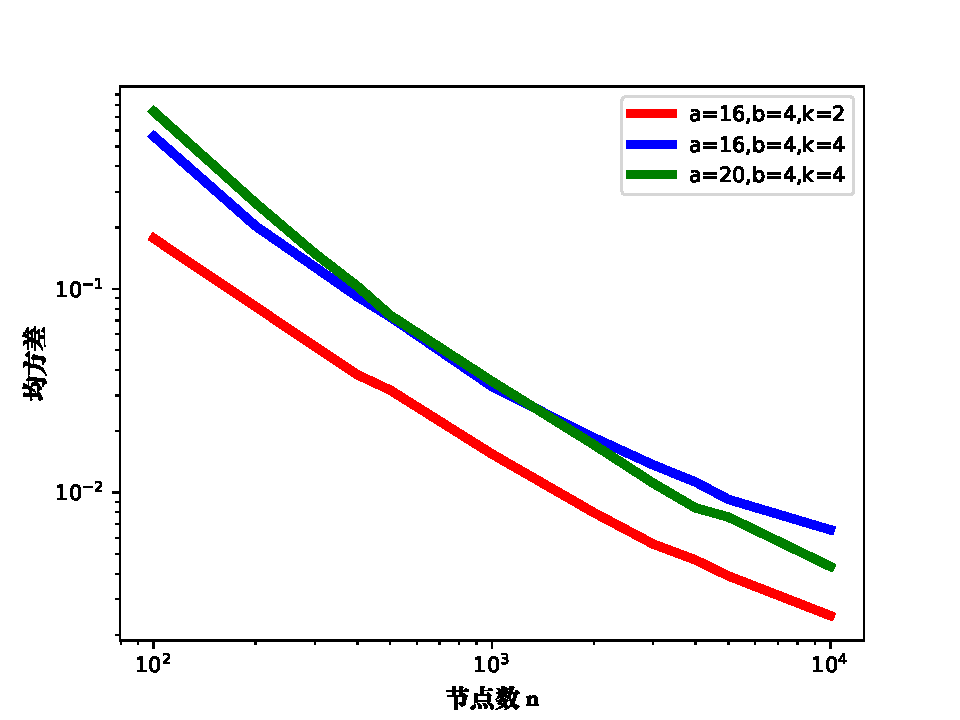
\includegraphics[width=0.6\textwidth]{estimator-error-2023-02-07.pdf}
		\caption{ $\hat{a}, \hat{b}$ 的估计误差随
		$n$ 的变化规律 }\label{fig:estimator}
\end{figure}

\section{基于玻茨模型的社群发现算法}\label{sec:potts}
\subsection{算法描述}
类似于\ref{sec:sibm_model}节
介绍的SIBM模型,我们将
随机块模型
与 \ref{sec:ising} 节介绍的 玻茨模型
复合起来可得到随机块-玻茨模型。该模型可以看成是SIBM模型的推广,
每个节点由两状态变成了多状态。由于我们的研究重点并非
从随机块-玻茨模型的多个样本恢复节点的原始标签,而是利用
玻茨模型对随机块模型进行社群发现,因此我们首先给出
由随机块模型生成的图上定义的玻茨模型:
\begin{definition}\label{def:ising}
	给定从$\SSBM(n,k,\A,\B)$ 中生成的随机图 $G$,
    定义在$G$上的玻茨模型($k$个状态的伊辛模型)带有两个参数 $\gamma,\beta>0$,
	并且是关于状态向量$\sigma\in W^n$ 的概率分布
。该分布的概率质量函数为
\begin{align} \label{eq:isingma}
	P_{\sigma|G}(\sigma=\bar{\sigma})=\frac{\exp(-\beta H(\bar{\sigma}))}{Z_G(\gamma,\beta)}
	\end{align}
其中能量函数$H(\bar{\sigma})$的定义是
\begin{equation}\label{eq:energy}
	H(\bar{\sigma}) := \gamma \frac{\log n}{n} \sum_{\{i,j\}\not\in E(G)} \delta(\bar{\sigma}_i, \bar{\sigma}_j)
	- \sum_{\{i,j\}\in E(G)} \delta(\bar{\sigma}_i, \bar{\sigma}_j)
	\end{equation}
	
	$P_{\sigma|G}$ 中的下标表示该分布依赖于$G$,
    $Z_G(\gamma,\beta)$ 是该分布的归一化常数。
\end{definition}

式\eqref{eq:isingma}中
各符号的含义同式\eqref{eq:canonical_ensemble}。
而表示汉密尔顿能量的式\eqref{eq:energy}
则是式\eqref{eq:ising_modified}的推广。
当  $k=2$ 时 式 \eqref{eq:energy}
在评注\ref{rem:equivalence_H_energy}的意义下
退化成 式 \eqref{eq:ising_modified}。 

这里的能量函数$H(\bar{\sigma})$ 同样有两部分组成:
没有边相连的节点之间排斥力的势能和
有边相连的节点之间吸引力的势能。
$\gamma$ 参数衡量了两种势能之间的比率而
$\frac{\log n}{n}$ 则是对由于边的数量不均匀造成两种势能量阶不同的修正项,
因为两节点间有边相连的概率仅为 $O(\frac{\log n}{n})$。

定义 \ref{def:ising} 实际上给出了一个估计$X$的随机算法 $\hat{X}^*$。
这里,$\hat{X}^*$ 表示产生于玻茨模型的一个样本,
记作$\hat{X}^* \sim \textrm{Potts}_G(\gamma, \beta)$。
下面我们首先研究$\hat{X}^*$实现精确恢复的条件及误差上界,
而关于如何进行玻茨模型的采样我们将在节进行讨论。
\subsection{误差的渐近性质}
沿用评注\ref{rem:metric_exact_recovery} 中的记号,
使用$\hat{X}^*$估计$X$在精确恢复度量下的错误概率
记为 $P_e(\hat{X}^*) := \sum_{G \in \cG_n} P_G(G) P_{\sigma | G}(S^c_k(X))$。
类似定理\ref{thm:sibm_phase_trans}中关于 SIBM 模型的讨论,
玻茨模型的两个参数$(\gamma, \beta)$ 的取值
对$P_e(\hat{X}^*)$
也有着决定性的作用。
当它们取合适的值时, 
$ P_e(\hat{X}^*)\to 0$,
随机块模型的精确恢复可以实现。
反之,如果 $(\gamma, \beta)$ 取其他值时,
$P_e(\hat{X}^*) \to 1$。
这两种情况可总结为如下的定理:

\begin{theorem}\label{thm:phase_transition}
	假设 $\sqrt{a} - \sqrt{b} > \sqrt{k}$,
	定义函数 $g(\beta)$ 和 $ \tilde{g}(\beta)$ 如下:
	\begin{equation}
		\label{eq:g_beta_main_article}
		g(\beta) = \frac{be^{\beta} + a e^{-\beta}}{k} - \frac{a+b}{k} +1
	\end{equation}
	且
	\begin{equation}
		\label{eq:g_tilde_beta_main_article}
	\tilde{g}(\beta) = \begin{cases}
	g(\beta) & \beta \leq \bar{\beta} = \frac{1}{2}\log \frac{a}{b} \\
	g(\bar{\beta}) = 1 - \frac{(\sqrt{a} - \sqrt{b})^2}{k} & \beta > \bar{\beta}
	\end{cases}
	\end{equation}
	其中
	$\bar{\beta} =  \displaystyle\arg\min_{\beta > 0} g(\beta)$。
	令 $\beta^*$ 定义成
	\begin{equation}\label{eq:beta_star}
	\beta^* = \log\left(\frac{a + b - k - \sqrt{(a + b - k)^2 - 4 a b)}}{2  b}\right)
	\end{equation}
	可以验证 $\beta^*$ 是方程 $g(\beta) = 0$ 的解 并且满足  $\beta^* < \bar{\beta}$。
	则取决于 $(\gamma, \beta)$ 如何取值,对于给定的 $\epsilon > 0$, 
	$G\sim \SSBM(n, k, \A, \B)$, $\hat{X}^* \sim \textrm{Potts}_G(\gamma, \beta)$,
	当 $n$ 充分大时, 我们有:
	\begin{enumerate}
	\item 当 $\gamma > b$ 且 $\beta > \beta^*$ 时,$P_e(\hat{X}^*) \leq n^{\tilde{g}(\beta)/2 + \epsilon}$;
	\item 当 $\gamma > b$ 且 $\beta < \beta^*$ 时,$P_a(\hat{X}^*) \leq (1+o(1))\max\{n^{g(\bar{\beta})}, n^{-g(\beta) + \epsilon}\}$;
	\item 当 $\gamma < b$ 时,对于任意给定的 $C>0$	均有 $P_a(\hat{X}^*) \leq \exp(-C n)$。
	\end{enumerate}
\end{theorem}

\begin{figure}[H]
	\begin{subfigure}{0.43\textwidth}
		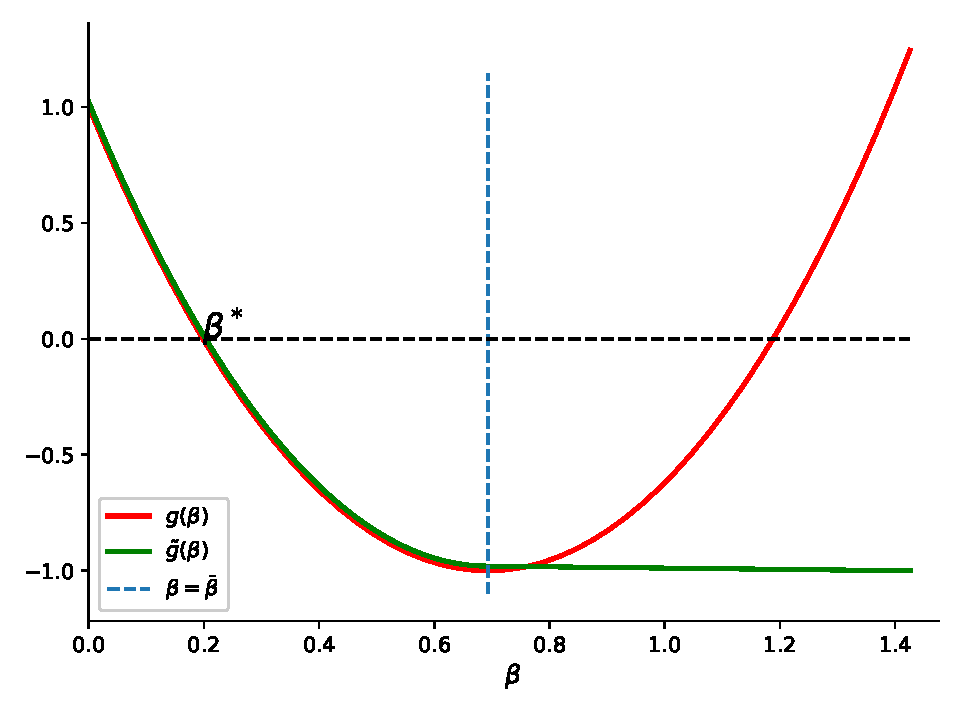
\includegraphics[width=\textwidth]{g-16-4-2.pdf}
		\caption{当 $a=16,b=4,k=2$时,$g(\beta)$和
		$\tilde{g}(\beta)$的函数图像}\label{fig:g}
	\end{subfigure}~
	\begin{subfigure}{0.55\textwidth}
		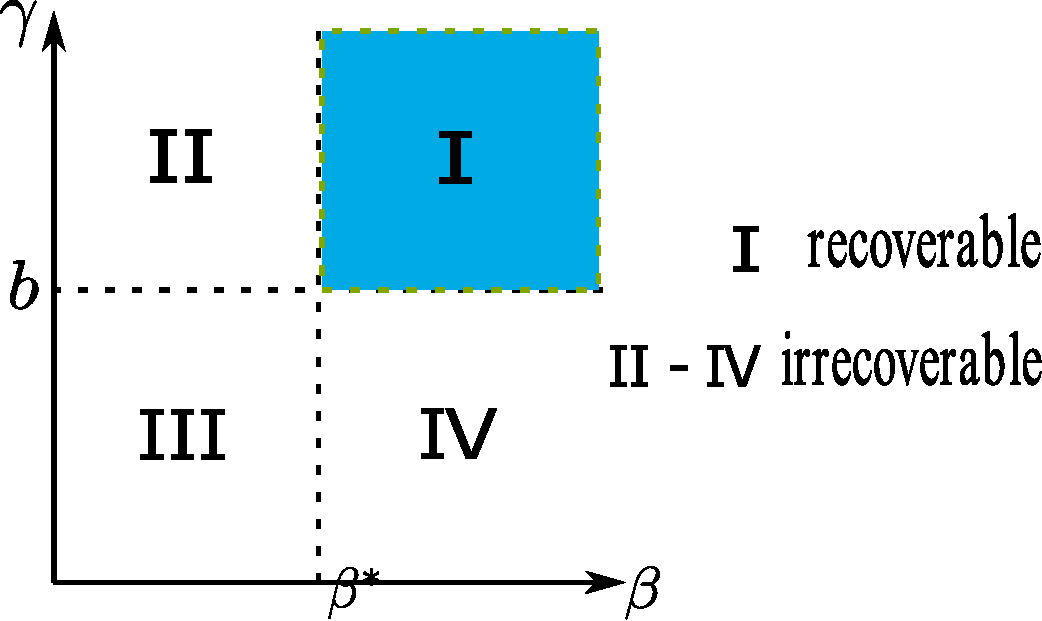
\includegraphics[width=\textwidth]{phase_trans.pdf}
		\caption{
			在 $(\beta, \gamma)$ 平面内
			相变区域图示。
			随机块模型的精确
			恢复仅在区域 I 可实现。}\label{fig:pt}
	\end{subfigure}
	\caption{定理 \ref{thm:phase_transition}
	的图示}
	\label{fig:phase_transition_theorem_illustration}
\end{figure}
\begin{remark}
	在式\eqref{eq:g_beta_main_article} 中,我们首次引入了
	$g(\beta)$ 这个函数,该函数是由矩生成函数导出的,
	其信息学含义为速率函数的凸共轭函数,我们具体将在后面的 \ref{sub:rate_function} 小节进行介绍。
\end{remark}
与式\eqref{eq:beta_star_sibm}的情形类似,注意到条件$\sqrt{a} - \sqrt{b} > \sqrt{k}$保证了
式\eqref{eq:beta_star}中的根号下的项非负。
这个条件来自于定理\ref{thm:sbmk_phase_transition},
保证了随机块模型本身精确恢复可实现。


通过简单的计算可知,对于 $\beta> \beta^*$ 我们有
$\tilde{g}(\beta) < 0$ 而 对于 $\beta < \beta^*$有
$g(\beta)>0$。
另外,由 $\sqrt{a} - \sqrt{b} > \sqrt{k}$ 可知
$g(\bar{\beta}) < 0$。
$g(\beta), \tilde{g}(\beta)$ 的图像
如图 \ref{fig:phase_transition_theorem_illustration}a 所示。
因此, 对于充分小的
$\epsilon$ 并且当 $n \to \infty$,
定理\ref{thm:phase_transition} 中给出的上界
均至少以多项式的速度趋向于 $0$。
从而定理\ref{thm:phase_transition} 
刻划了
玻茨模型的相变性质。
如图\ref{fig:phase_transition_theorem_illustration}b所示
, 对于玻茨模型, 只有参数$(\beta, b)$落在区域I时,
随机块模型的精确
恢复才能实现。



定理 \ref{thm:phase_transition} 中的$k=2$与
定理 \ref{thm:sibm_phase_trans} 中的$m=1$时
的结论是一致的。此外,
定理\ref{thm:phase_transition}
也可以从$\sigma$的边缘分布的角度理解。
玻茨模型取到某个特定状态$\bar{\sigma}$的概率为
 $\sigma: P_{\sigma}(\sigma =\bar{\sigma})
=\sum_{G \in \cG_n}P_G(G)P_{\sigma |G}(\sigma=\bar{\sigma})$.
\newglossaryentry{not:sigma_nearest_to_the_latter}
{
  type=notation,
  name={\ensuremath{D(\sigma, \sigma')}},
  description={$\sigma$ 相比于它的所有置换其本身离 $\sigma'$ 最近
  这个事件}
}
我们用符号 \gls{not:sigma_nearest_to_the_latter} 表示 \glsdesc{not:sigma_nearest_to_the_latter}
。
也即
\begin{equation}
	\label{eq:D_sigma_sigma_prime}
D(\sigma, \sigma') := \{ \sigma = \arg\min_{f \in S_k} \Dist(f(\sigma), \sigma')  \}
\end{equation}

则 定理 \ref{thm:phase_transition} 
对边缘分布 $P_{\sigma}$ 蕴含着如下的论断
:
\begin{corollary}\label{cor:phase4}
假设 $\gamma > b$, 取决于 $\beta$ 的取值我们有
\begin{enumerate}
	\item 当 $\beta > \beta^*$时,$P_{\sigma}(\sigma = X | D(\sigma, X))  = 1-o(1)$;
	\item 当 $\beta < \beta^*$时,$P_{\sigma}(\sigma = X | D(\sigma, X))  = o(1)$。
\end{enumerate}
\end{corollary}

下面我们简单阐述下 定理 \ref{thm:phase_transition} 证明的思路。
该思路主要通过对翻转一个状态的前后能量差的分析来估计概率的主项。
下面的引理总结了翻转一个状态汉密尔顿能量的变化:
\begin{lemma}\label{lem:lemmaDiff}
	假设 $\bar{\sigma}'$ 仅在第$r$个位置上与 $\bar{\sigma}$ 不同,
	差别为 $\bar{\sigma}'_r = \omega^s \cdot \bar{\sigma}_r$。
	则 $\bar{\sigma}'$ 和 $\bar{\sigma}$ 的能量差为
\begin{align}
	H(\bar{\sigma}') - H(\bar{\sigma}) &= (1+\gamma \frac{\log n}{n})\sum_{i \in N_r(G)} J_s(\bar{\sigma}_r, \bar{\sigma}_i)
	\notag \\
	&+ \gamma \frac{\log n}{n} (m(\omega^s \cdot \bar{\sigma}_r)-m(\bar{\sigma}_r)+1) \label{eq:DeltaH}
	\end{align}
	上式中 $m(\omega^j) := |\{i \in [n] | \bar{\sigma}_i = \omega^j | \}$, 
	$N_r(G):=\{j | (r, j) \in E(G) \}$ 表示节点$r$
	的邻居节点,而 $J_s(x, y) = \delta(x, y) - \delta(\omega_s \cdot x, y)$.
\end{lemma}
\begin{remark}\label{re:energy_diff}
	当 $\bar{\sigma}'$ 与 $X$ 仅在位置 $r$
	上不同时, 在引理 \ref{lem:lemmaDiff}
	中取$\bar{\sigma}=X$,
	结合条件  $|\{v \in [n] : X_v = u\}| = \frac{n}{k}$,
	有 $m(\omega^s \cdot \bar{\sigma}_r)
	=m(\bar{\sigma}_r)$,
	进而:
	\begin{equation}\label{eq:energy_diff}
	H(\bar{\sigma}') - H(X) = (1+\gamma \frac{\log n}{n})(A^0_r - A^s_r) + \gamma\frac{\log n}{n}
	\end{equation}
	其中 $A^s_r$ 定义成
	$A^s_r := |\{j \in [n]\backslash \{r\}: \{j, r\} \in E(G), X_j = \omega^s \cdot X_r \}|$。
	因为$G$中各边的存在与否是独立的,
	对于 $s\neq 0$
	我们有 $A^s_r \sim \Binom \left(
	  \frac{n}{k}, \B \right) $,
	而 $A^0_r \sim \Binom
	\left(
	  \frac{n}{k}-1, \A \right)$。	
\end{remark}
考虑到:
\begin{equation}\label{eq:Pratio}
\frac{P_{\sigma |G } (\sigma = \bar{\sigma}')}{P_{\sigma |G } (\sigma = \bar{\sigma})}
= \exp(-\beta(H(\bar{\sigma}') - H(\bar{\sigma})))
\end{equation}
因此引理 \ref{lem:lemmaDiff} 提供了用以比较两个相邻状态的    概率
的方法。当 $n$充分大时,我们注意到式
\ref{eq:Pratio} 右端化为$\exp(-\beta (A_r^0 - A_r^s))$。
而如果我们对其取期望,则可以得到
\begin{equation}\label{eq:expect_A_r_0_s}
	\E[\exp(-\beta (A_r^0 - A_r^s))] \sim n^{g(\beta)-1}
\end{equation}
也即 $g(\beta)$与两个二项分布差$A_r^0 - A_r^s$的矩生成函数有关。



另外, 我们注意到 因为图的边的数量是稀疏的,每个节点
平均有 $O(\log n)$ 个相连的邻居节点。
按照式 \eqref{eq:DeltaH} 
计算能量差的时间复杂度也是 $O(\log n)$。

当 $H(\bar{\sigma}') > H(\bar{\sigma})$ 时, 
由式\eqref{eq:Pratio} 可得
$P_{\sigma | G}(\sigma = \bar{\sigma}')$
小于
$P_{\sigma | G}(\sigma = \bar{\sigma})$。
粗略而言, 如果
$ \sum_{\Dist(\sigma', X)=1}\exp(-\beta(H(\bar{\sigma}') - H(X))) $
收敛到零,
我们可以预期,与$S_k(X)$不同的所有其他状态的概率收敛到零。
与之相反, 如果
$ \sum_{\Dist(\sigma', X)=1}\exp(-\beta(H(\bar{\sigma}') - H(X))) $
趋于无穷大,
则 $P_{\sigma}(S_k(X))$ 趋于零。
此种分析展示了证明定理 \ref{thm:phase_transition}的
主要思路。应用这一思路,由
\eqref{eq:expect_A_r_0_s}式,
当$n$充分大时,$ \sum_{\Dist(\sigma', X)=1}\exp(-\beta(H(\bar{\sigma}') - H(X))) $
的数学期望为 $n^{g(\beta)}$,这也部分说明了
$g(\beta)$出现在定理\ref{thm:phase_transition}表述中的原因。
\subsection{速率函数}\label{sub:rate_function}
在\eqref{eq:expect_A_r_0_s} 中我们指出了$g(\beta)$与
二项分布差$A_r^0 - A_r^s$的矩生成函数有关,本节将进一步挖掘
其信息论的含义,即$g(s)-1$是速率函数$g(a,b,s)$的凸共轭函数。

首先,通过切尔诺夫不等式的方法(证明见附录引理\ref{lem:enhanced_fb}),
我们有
\begin{equation}\label{eq:introduction_g_a_b_eps}
  P_G(A_r^s - A_r^0 \ge t  \log n) 
	\le  \exp\Big(-\log n
	\left(
   \frac{1}{k} g(a,b,kt) + O((\log n)^{-\delta}) \right)\Big)
\end{equation}
其中 函数 $g(a,b,\epsilon)$ 定义为
\begin{equation}  \label{equation:g}
  g(a,b,\epsilon) \triangleq a + b - \sqrt{\epsilon^2 + 4ab} + \epsilon \log \frac{\epsilon + \sqrt{\epsilon^2 + 4ab}}{2b}
\end{equation}
其等价形式亦可参见 \citet{abbe2015exact} 中的 式 (43)
。
易验证 $\frac{g(a,b,kt)}{k}=-[f_{\beta}(t)-\beta t -1]$。
\begin{remark}\label{re:g_beta}
实际上 $g(a,b,s)$ 和 $g(s)-1$ 互为凸共轭函数。

利用凸共轭函数的概念,
下面我们引入大偏差理论中的 Gärtner Ellis 定理
来获得 $g(a,b,\epsilon)$。Gärtner Ellis 定理是
Cramér 定理(定理\ref{thm:cramer})的推广,其一般情形下的表述可参见
\citet{dembo2009large}。
我们这里仅给出 Gärtner Ellis 定理的一个特例形式。

令 $S_n$ 为随机变量的序列,
$\gamma_n >0, \lim_{n\to \infty}\gamma_n \to 0$.
$\Lambda_n(t)=\log \E[\exp(t S_n)]$ 代表 $S_n$ 的对数矩生成函数 (log-MGF)。
假设对于任意的 $t$,
$\Lambda(t) =\lim_{n\to \infty} \frac{1}{\gamma_n}\Lambda_n(\gamma_n t)$
存在。 令 $\Lambda^*$ 是 $\Lambda$ 的共轭函数。
则对于任意 紧集 $\Gamma \subset \mathbb{R}$,
我们有
\begin{equation}\label{eq:gartner_ellis}
\lim_{n\to \infty} \frac{1}{\gamma_n}\log P(S_n \in \Gamma) = -\inf_{s \in \Gamma} \Lambda^*(s)
\end{equation}
仿照 Cramér 定理中速率函数的概念,这里我们也把$\Lambda^*(s)$叫做速率函数。

下面我们应用式 \eqref{eq:gartner_ellis}
导出 $g(a,b,\epsilon)$ 的
表达式。
我们取 $\gamma_n= \log n$ 且 $\gamma_n S_n = \sum_{i=1}^n Y_i$,$Y_i=Z_i - W_i$,
$Z_i, \dots, Z_n$ 是 i.i.d. $\Bern(\B)$ 而 $W_1, \dots, W_n$ 是 i.i.d. $\Bern(\A)$。
$Y_i$ 的概率质量函数为 $[(1-q)p, qp+(1-p)(1-q), q(1-p)]$,对应 $[-1,0,1]$ 三个取值。
首先我们计算得到 
$\Lambda(t) = \lim_{n\to \infty} \frac{n}{\log n} \log \E[\exp(t Y_1)]
=-a-b+be^t  + ae^{-t}$. 由 $\Lambda^*(s) = \sup_{t\in\mathbb{R}} st - \Lambda(t)$,
我们进一步得到 $\Lambda^*(s) = g(a,b,s)$。

在我们的问题中, $\Gamma=[t, +\infty)$ 而 $k$ 取 1。
考虑到 $\Lambda^*(s)$  是$[0,+\infty)$ 上的增函数,
我们有
\begin{equation}
  \lim_{n\to \infty} \frac{1}{\log n} P(B_{\bar{\sigma}}-A_{\bar{\sigma}}\ge t \log n)
  = g(a,b,t)
\end{equation}
特别地,当$t=0$ 时, $g(a,b, 0) = (\sqrt{a} - \sqrt{b})^2$。
\end{remark}
\section{基于能量最小化的社群发现算法}\label{sec:em}
因为 $\beta^*$ 和 $n$ 无关,
当 $\gamma>b$ 时,
我们可以选取一个足够大的 $\beta$ 使得
$\beta > \beta^*$,
则 由 定理\ref{thm:phase_transition}, 当$n$充分大时 $\sigma \in S_k(X)$ 几乎必然发生。
这蕴含了 $P_{\sigma | G}(\sigma = X)$
对于几乎所有的 从 SBM 采样的图  $G$来说 取得最大值。
因此
相比于从伊辛模型中采样的方法,我们可以直接最大化条件概率,以
找到概率最大值的状态。
等价地, 我们可以通过最小化 \eqref{eq:energy}式的方式来获得状态的估计量:
\begin{equation}\label{eq:hatX}
\hat{X}' := \arg\min_{\bar{\sigma} \in W^n} H(\bar{\sigma})
\end{equation}

在 \eqref{eq:hatX} 中, 我们让 $\bar{\sigma}$ 在 $W^n$ 中取值。
因为我们已知 $X$取各个标签的位置数相等,即对于每个标签值 $u$
有 $|\{v \in [n] : X_v = u\}| = \frac{n}{k}$,
我们可以把搜索空间限制到
$W^*:= \{\sigma\in W^n \big\vert |\{v \in [n] : \sigma_v = \omega^s\}| = \frac{n}{k}, s=0,\dots, k-1 \}$
上。
当 $\sigma \in W^*$ 时, 最小化 $H(\sigma)$ 等价于:
\begin{equation}\label{eq:hatX_double_prime}
\hat{X}'' := \arg\min_{\sigma \in W^*} \sum_{\{i,j\} \not\in E(G) } \delta(\sigma_i, \sigma_j)
\end{equation}
其中最小值是不同社群之间的最小分割。

当 $\hat{X}'' \neq X$ 时,
我们必须有  $\Dist(\hat{X}'' ,X)\geq 2$
以满足 硬约束 $\hat{X}'' \in W^*$。
此外,估计量 $\hat{X}''$ 是无参的而 $\hat{X}'$的值受
参数 $\gamma$ 的影响。
在
$\hat{X}'$ 的表达式中出现的额外的参数 $\gamma$ 可视为
某种整数规划的拉格朗日乘子。
因此,通过引入惩罚因子项和将搜索空间从$W^*$ 扩大 到$W^n$
,求解 $\hat{X}'$
的优化问题 转变为 $\hat{X}''$的优化问题。

当 $\beta > \bar{\beta}$ 时,
$\tilde{g}(\beta)$ 是一个常数。
因此,从 Theorem \ref{thm:phase_transition} 中我们可以获得的关于
伊辛模型的估计量 $\hat{X}^*$ 最紧的上界
是  $n^{g(\bar{\beta})/2}$。

对于 $\hat{X}'$ 和 $\hat{X}''$ 这两个估计量,
我们可以获得 更紧的误差上界。我们把这一结果总结为如下定理:
\begin{theorem}\label{thm:error_rate}
当 $\sqrt{a} - \sqrt{b} > \sqrt{k}$ 时,
对于充分大的 $n$,我们有 
\begin{enumerate}
	\item 若 $\gamma > b$, $P_G(\hat{X}' \not\in S_k(X)) \leq (k-1+o(1))n^{g(\bar{\beta})}$;
	\item $P_G(\hat{X}'' \not\in S_k(X)) \leq ((k-1)^2+o(1))n^{2g(\bar{\beta})}$。
\end{enumerate}
\end{theorem}
因为 $g(\bar{\beta})<0$, 我们有大小关系 $n^{2g(\bar{\beta})} < n^{g(\bar{\beta})} < n^{g(\bar{\beta})/2}$。
从而 定理 \ref{thm:error_rate} 说明了在三个估计量中,
$P_e(\hat{X}'')$ 
的上界最紧。
这可以直观地理解为搜索空间缩小的结果。
定理\ref{thm:error_rate} 的证明技术是对于 $\Dist(\bar{\sigma}, X) \geq 1$,考虑事件
$H(X) > H(\bar{\sigma})$发生的概率。
\newglossaryentry{bool_ineq}{name=布尔不等式, description={Boole's inequality}}
然后通过\gls{bool_ineq}, 这些概率可以相加。
关于估计量 $\hat{X}''$ 误差上界的研究早在\citet{abbe2015exact} 的工作中即有涉及,
但他只得到了一个比较松的上界 $n^{g(\bar{\beta})/4}$,且仅针对 $k=2$ 的情形。
对于一般的情形,
当条件
$\sqrt{a} - \sqrt{b} > \sqrt{k}$ 满足时,考虑到
$\tilde{g}(\beta) = 1- \frac{(\sqrt{a} - \sqrt{b})^2}{k}$,
定理 \ref{thm:error_rate} 说明了  $\hat{X}'$ 和 $\hat{X}''$
均可实现
精确恢复。


估计量 $\hat{X}'$ 有一个参数 $\gamma$。
当 $\gamma$ 取特定的值时, $\hat{X}'$在渐近情形下
可以等价于 最大似然估计或最大模块度估计。
以下分析从直观地角度说明了
这种联系。

通过最大化对数似然函数可得到最大似然估计量。
由 \eqref{eq:GmL} 式,该似然函数可以进一步写成:
\begin{equation}\label{eq:PG_energy}
	\log P_G(Z=z|X=\sigma) = -\log\frac{a}{b} \cdot H(\sigma) + C
\end{equation}

这里 在$H(\sigma)$ 的表达式中 参数 $\gamma$ 的取值满足
\begin{equation}\label{eq:special_gamma_ML}
	\gamma \frac{\log n}{n} = \frac{1}{\log(a/b)}
	\left(\log \left(1-\B \right) - \log \left(1-\A \right) \right)	 
\end{equation}

而 $C$ 是一个和 $\sigma$ 无关的常数。
当 $n$ 充分大时,我们有 $\gamma \to \gamma_{ML} := \frac{a-b}{\log(a/b)}$。   
也即,
当 $\gamma = \gamma_{ML}$时,
最大似然估计量 渐近等价于 $\hat{X}'$。

这里我们顺便得到了最大似然算法和最小割问题在有$W^*$约束
下的等价性,这个等价性不需要渐近的条件也成立。
因为最大似然算法首先等价于极小化能量$H(\sigma)$,
$\gamma$从\eqref{eq:special_gamma_ML}式中取值。其次,
由\eqref{eq:hatX_double_prime}式,极小化能量$H(\sigma)$
等价于$\min \sum_{\{i,j\} \not\in E(G) } \delta(\sigma_i, \sigma_j)$
因为在$W^*$的约束下,
$\sum_{1<i<j<n} \delta(\sigma_i, \sigma_j)$
是一个常数,\eqref{eq:hatX_double_prime}式又等价于
$-\sum_{ \{i,j\} \in E} \delta(\sigma_i, \sigma_j)$,
其与 \eqref{eq:minimum_k_cut}式只相差一个常数。


最大模块度估计量通过最大化 \ref{eq:Q}式而得到。
忽略常数项,关于标签向量 $\sigma$的模块度 $Q$
可以写成:
\begin{align}
Q(\sigma) = -\sum_{\{i,j\} \not\in E(G) } \frac{d_i d_j}{2 |E|}\delta(\sigma_i,\sigma_j) 
+ \sum_{\{i,j\} \in E(G) } (1 - \frac{d_i d_j}{2 |E|}) \delta(\sigma_i,\sigma_j)  \label{eq:Qtransform}
\end{align}

当$n$充分大时,平均意义上我们有 $d_i \sim  \frac{(a+(k-1)b)\log n}{k}, |E| \sim \frac{1}{2}n d_i$。
因此,我们有
$\frac{d_id_j}{2|E|} \to \gamma_{MQ} \frac{\log n}{n} $。
从 \eqref{eq:Qtransform}式我们可以看到,
当 $\gamma = \gamma_{MQ} = \frac{a+(k-1)b}{k}$ 且 $n\to \infty$时,
$Q(\sigma) \to -H(\sigma)$。
也即,当$\gamma = \gamma_{MQ}$ 时,
最大模块度估计量渐近等价于
$\hat{X}'$ 。


通过$a>b$和 当$x>1$时的不等式 
 $x-1>\log x $,我们可以验证
  $\gamma_{MQ} >b$ 且  $\gamma_{ML} > b$。
  这说明 了
  最大似然估计和最大模块度估计都满足
  定理\ref{thm:error_rate}所述的精确恢复条件 $\gamma > b $。

\section{基于梅特罗波利斯采样的社群发现算法}\label{sec:ms}

由定理\ref{thm:phase_transition}可知,
如果我们直接从玻茨模型 \eqref{eq:isingma} 式中采样,那么得到的样本大概率
与$X$一致。
然而,当$n$非常大时,按照分布\eqref{eq:isingma}式精确采样是困难的,
因为状态空间的状态总数随着$n$以
$k^n$的速率指数增大。
因此,一定程度的近似是必要的,
为此我们可以借助 \ref{sec:ising} 节介绍的梅特罗波利斯算法。 
经过若干次初始迭代后,梅特罗波利斯算法
每次产生的样本可视为从玻茨模型 采样的结果。
这个论断相关的理论研究主要是基于马尔可夫链。
在某些一般性的条件下,
梅特罗波利斯算法生成的样本收敛到
马尔可夫链的稳态并且该稳态分布即为要近似的分布。
针对伊辛模型的不同变体,
之前的许多工作都表明了梅特罗波利斯算法采样的收敛性\cite{diaconis1998we}。
这里我们假设可以推广类似的收敛性结果可以推广到
形如 \eqref{eq:isingma} 式中描述的玻茨模型。

我们对算法 \ref{alg:Metropolis}
进行改写即可得到针对我们的模型和能量表达式 \eqref{eq:energy},
的算法 \ref{alg:m}。
算法 \ref{alg:m} 要求
社群数量 $k$ 和参数 $\beta, \gamma$ 事先给定。
并且,根据定理\ref{thm:phase_transition},我们需选取  $\beta>\beta^*, \gamma > b$
\footnote{ $\beta^*$ 的定义参见式 \eqref{eq:beta_star} }
。
这里的 $a, b$
可以通过 定理 \ref{thm:ab12} 中提出的估计量$\hat{a},\hat{b}$进行近似。
此外,算法的迭代次数  $N$
也需事先确定。
\begin{algorithm}[H]
	\caption{针对玻茨模型的梅特罗波利斯算法} \label{alg:m}
	输入: 图 $G$, 参数 $\beta$、$\gamma$ \\
	输出: $\hat{X} = \bar{\sigma}$
	\begin{algorithmic}[1]
		\STATE 随机初始化 $\bar{\sigma} \in W^n$ %\vskip 0.5em
		\FOR{$i=1,2,\dots, N$}
		\STATE 根据引理 \ref{lem:lemmaDiff},
		随机选取 $s, r$ 并得到新的状态
		 $\bar{\sigma}'$
		 %\vskip 0.5em
		\STATE 通过 \eqref{eq:DeltaH} 计算 $\Delta H(r,s) = H(\bar{\sigma}') - H(\bar{\sigma})$ %\vskip 0.5em
		\IF{$\Delta H(r,s)<0$}
		\STATE $\sigma_r \leftarrow w^s \cdot \sigma_r$ %\vskip 0.5em
		\ELSE
		\STATE 以概率 $\exp(-\beta \Delta H(r,s))$ 使得
			$\sigma_r \leftarrow w^s \cdot \sigma_r$,
			否则保持原状。 %\vskip 0.5em
		\ENDIF %\vskip 0.5em
		\ENDFOR
	\end{algorithmic}
\end{algorithm}
 由 引理 \ref{lem:lemmaDiff} , $\Delta H(r,s)$ 的计算需要 $O(\log n)$ 的时间。
有研究针对某种特殊的伊辛模型指出
$N=O(n\log n)$ 即可得到估计得比较好的样本\cite{mcmc}。
对于我们的模型,由于我们并不清楚 $ N = O(n\log n)$ 是否足够,
因此我们在数值实验中经验地选取 $N=O(n^2)$。
则 算法 \ref{alg:m} 总的时间复杂度为 $O(n^2 \log n)$。



借助梅特罗波利斯算法,
下面我们通过实验验证 定理 \ref{thm:phase_transition} 中的 $\gamma > b$的情形。
我们选取了 $n=9000, k=2$,
通过蒙特卡罗采样的方法,我们可以得到准确率的经验计算公式为
$P_a(\hat{X}^*) = \frac{1}{m_1m_2}\sum_{i=1}^{m_1} \sum_{j=1}^{m_2} \mathbf{1}[\hat{X}^* = \pm X]$。
在这个公式中,
$m_1$ 是 由 SBM 模型产生的随机图的次数,而
$m_2$ 是 对于一个特定的图,由算法\ref{alg:m} 生成的连续样本的数量。
我们选取 $m_1=2100,m_2=6000$。这样的取值已相当大,
且由大数定律
可达到 $P_a(\hat{X}^*)$ 的好的估计。
$P_a(\hat{X}^*)$ 随 $\beta$的变化在 图 \ref{fig:erh}
中给出。

\begin{figure}[ht!]
	\centering
		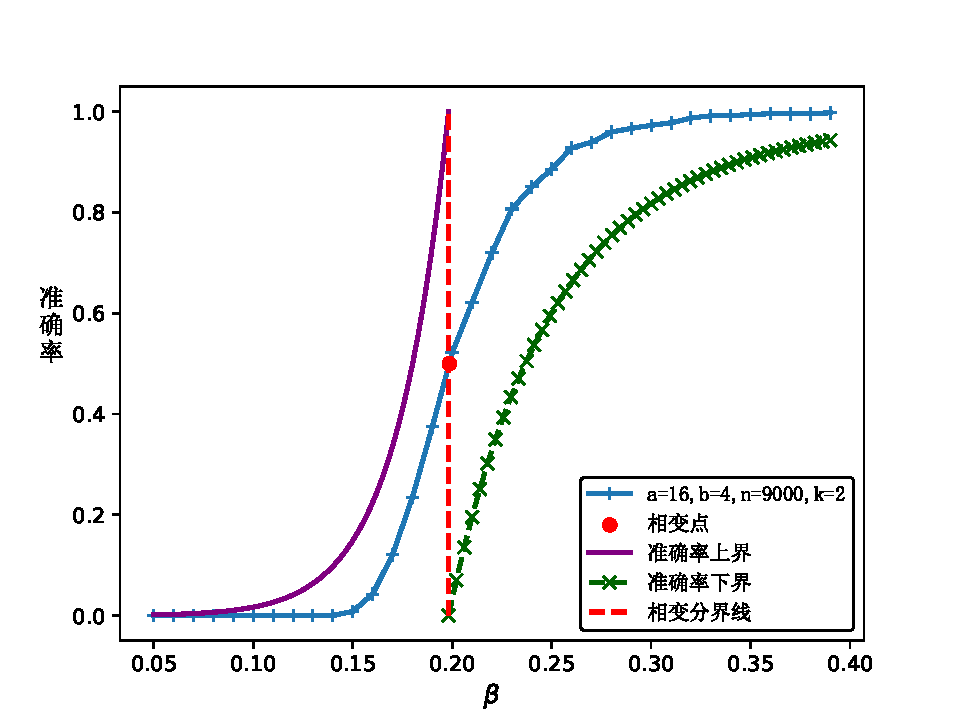
\includegraphics[width=0.6\textwidth]{beta_trans-2020-11-28.pdf}
		\caption{使用 $\hat{X}^*$ 进行社群发现精确恢复的准确率}\label{fig:erh}
\end{figure}


竖线 ($\beta=\beta^* \approx 0.198$),
是 从 \eqref{eq:beta_star} 式计算得到的, 
代表了相变的临界值。
图 \ref{fig:erh}中的坐标点 $(0.199,\frac{1}{2})$
可视为通过实验估计出的
相变点,它的横坐标接近
$\beta^*$。
绿线 $(\beta, n^{g(\beta)/2})$ 
表示当 $\beta>\beta^*$ 时准确率的理论下界,
而紫线
$(\beta, n^{-g(\beta)})$ 
表示当 $\beta<\beta^*$ 时准确率的理论上界。
仿真实验得到的相变曲线(蓝线)恰好介于此两线之间。
当 $n$ 变得更大时,可预见
相变曲线 将接近阶跃函数,该函数的值在
$\beta=\beta^*$ 处
从 0 跳变到 1。
\section{本章小结}
在本章中, 
我们首先给出了 随机块模型参数的一致估计量 (定理 \ref{thm:ab12}) 
来推断参数$a,b$,而推断出的参数可用于后续算法设计中。其次,我们分析了
三个随机块模型节点标签的估计量:它们分别是基于玻茨模型的采样、基于极小化汉密尔顿能量
以及基于极小化带约束的能量函数。
在定理 \ref{thm:phase_transition} 和 \ref{thm:error_rate}
中,我们给出了这三个估计量精确恢复的误差上界,并且研究了它们的误差上界之间的关系。
本章通过引入$k$状态的伊辛模型,
开辟了研究随机块模型精确恢复问题的新途径。
本章中涉及的模型和误差上界的分析技术,将成为下一章研究有额外信息的随机块模型
的基础。


\chapter{有额外信息的随机块模型}
\label{chap:sbmsi}
在本章中,我们首先引入我们研究的有额外信息的随机块模型
的定义。然后研究它的精确恢复的条件以及实现其精确恢复的半正定规划算法。

\section{精确恢复条件}
\label{sec:sbmsi_exact_recovery_condtion}
\newacronym{acr:sbmsi}{SBMSI}{Stochastic Block Model with side information}
带有额外信息的随机块模型(\gls{acr:sbmsi})
是 \ref{sec:sbm} 节介绍的
SSBM 模型的推广。这里我们在2个社群的随机块模型的
基础上引入额外信息。
除了图 $Z$ 和节点标签 $X$ 外,
第 $i$  个节点 ($1\leq i \leq n$) 
还含有 $m=\lceil \gamma \log n \rceil $ 个相关的数据样本 
$Y^{i}_{j}$, $j\in \{1,\ldots,m\}$。
这里,我们要求 $\gamma$ 是一个正整数。
若 $X_i=1$
这些样本 i.i.d. 采样自分布 $P_0$,若  $X_i=-1$ 则采样自 $P_1$。
这里假设 $P_0, P_1$ 两个分布函数均为定义在字母集$\mathcal{Y}$上的离散分布。
注意到 给定 标签 $X_i$,
对于 $i\in\{1,\ldots,n\}$,数据样本 $Y^{i}_{j}$, $j\in \{1,\ldots,m\}$ 与 $\{Z_{i,j}\}_{1\le i<j\le n}$ 独立。
 因此,在标签 $X$ 给定的情况下,
  $(\{Z_{i,j}\}_{1\le i<j\le n},\{Y^i_{j}\}_{1\le i\le n,1\le j\le m})$ 的联合分布为  
\begin{align}\label{eq:lh}
    &P(y=\{y^i_{j}\}_{1\le i\le n,1\le j\le m},z=\{z_{i,j}\}_{1\le i<j\le n}| (x_1,\ldots,x_n)) \nonumber\\
    &= \prod_{1\le i,j\le n}P(z_{i,j}|x_i,x_j)\prod_{i=1}^n \prod_{j=1}^m P(y^i_j|x_i), 
\end{align}
其中$\prod_{1\le i,j\le n}P(z_{i,j}|x_i,x_j)$ 可写成
\eqref{eq:mle_sibm} 式的形式。对于$P(z_{i,j}|x_i,x_j)$,其具体定义为
\begin{equation*}
    P  (z_{i,j}=1|x_i,x_j) = \begin{cases}
        p & \text{if } x_i = x_j \\
        q & \text{if } x_i\ne x_j
    \end{cases},
\end{equation*}
并且
\begin{equation*}
    P(y^i_j|x_i) = \begin{cases}
        P_0(y^i_j) & x_i = 1 \\
        P_1(y^i_j) & x_i = -1
    \end{cases}
\end{equation*}
 $P(\{x^i_{j}\}_{1\le i\le n,1\le j\le m},\{z_{i,j}\}_{1\le i<j\le n}| y_1,\ldots,y_n)$ 
 的条件分布 依赖于
 $n,m,p, q, P_0$ 和 $P_1$ 这些参数,因此我们把 SBMSI 写成 $\SBMSI(n,m,p,q,P_0,P_1)$ 的形式。
 给定由 $\SBMSI(n,m,p,q,P_0,P_1)$ 生成的图$Z$和数据$Y$, 我们的目标是恢复 出$X$。
 
 在有额外信息的条件下,
 我们仍使用能否精确恢复这一指标来衡量
 社群发现的可行性。与定义\ref{def:SSBMR}类似,
 若存在以$Z,Y$为输入变量的算法 $\hat{X}=\hat{X}(Z,Y)$
 使得当$n$增大时,
 错误概率
 $P_e:=P(\hat{Y} \neq Y)$ 趋向于 $0$,则称
 精确恢复可实现。

 \citet{abbe2015community}一文的3.2小节指出了一般SBM模型的精确恢复条件与多维泊松分布的关系。
在$k=2$的情形,我们要用到2维泊松分布,因此这里对其做一个简单的介绍。
有多种方式推广一维的泊松分布,这里我们使用的是如下定义:

\begin{definition}
    称 $(X,Y)$ 服从参数为 $(\lambda, \mu)$ 的二维泊松分布,
    如果其概率质量函数为:
    \begin{equation}
        P(X=k, Y=j) = \frac{\lambda^k \mu^j}{k! j!}
        e^{-\lambda - \mu}, k,j=0,1,\dots
    \end{equation}
    记为 $(X,Y) \sim \Pois(\lambda, \mu)$。
\end{definition}

有了2维泊松分布的定义式,我们下面给出
SBMSI 模型精确恢复的条件:
\begin{theorem}\label{thm:Pe}
    定义$I_+$ 为联合分布 $\textrm{Pois}(\frac{a}{2},\frac{b}{2})\times \underbrace{P_0 \times \dots \times P_0}_{\gamma}$
    与 $\textrm{Pois}(\frac{b}{2}, \frac{a}{2})\times \underbrace{P_1 \times \dots \times P_1}_{\gamma}$ 
    之间的切尔诺夫信息。    
    对于 $\SBMSI(n,m=\lceil \gamma \log n \rceil, p=a\frac{\log n}{n},q=b\frac{\log n}{n},P_0,P_1)$,
    如果 $I_+>1$,则精确恢复可实现;
    如果 $I_+ < 1$,
    则错误概率 $P_e$ 趋近于 $1$,精确恢复不可实现。
\end{theorem}

相比于 \citet{abbe17sideinfo} 中定理4的结论,
这里我们限制了类别数为2等条件,但允许采样数量 $m$ 为
$\lceil \log n \rceil $ 的整数倍。

对于一般的情形,SBMSI 模型精确恢复的 临界值 $I_+$ 并没有
显示表达式,但我们可以从切尔诺夫信息的定义出发得到 $I_+$ 的简化表达式,
由下述引理 \ref{lem:I_plus_expression} 给出。
该表达式更容易计算,且在定理\ref{thm:Pe}的证明中也会用到。

\begin{lemma}\label{lem:I_plus_expression}
\begin{align}\label{equation:I+}
    I_+ &=\frac{\lambda^* }{2} (a^{1-\lambda^* }b^{\lambda^* } -
    b^{1-\lambda^* }a^{\lambda^* })\log\frac{b}{a}+\frac{a+b}{2}\notag \\
    &-\frac{1}{2}(a^{1-\lambda^*}b^{\lambda^*} +
    b^{1-\lambda^* }a^{\lambda^* })+\gamma D(P_{\lambda^* }||P_0) 
	\end{align}
	其中
	\begin{equation}\label{eq:lambda}
    \lambda^* = \arg\min_{\lambda} \left[a^{1-\lambda}b^{\lambda} +
    b^{1-\lambda}a^{\lambda} + 2\gamma \log
    \left(\sum_{x\in \mathcal{X}}P^{1-\lambda}_0(x) P^{\lambda}_1(x)
    \right)
    \right]
\end{equation}
而 $P_{\lambda}$ 类似\eqref{eq:P_lambda_x} 式定义,为
\begin{equation}\label{eq:P_lambda_0_1}
    P_{\lambda}(x) = \frac{P_0^{1-\lambda}(x) P_1^{\lambda} (x)}
    {\sum_{x \in \mathcal{X}}P_0^{1-\lambda}(x) P_1^{\lambda} (x)}        
\end{equation}

\end{lemma}




当 $\gamma=0$ 时,由\eqref{eq:lambda}式 可得 $\lambda^*=\frac{1}{2}$,
则 $I_+=\frac{1}{2}(\sqrt{a}-\sqrt{b})^2$。
由定理\ref{thm:Pe},$\sqrt{a}-\sqrt{b} > \sqrt{2}$
时可精确恢复。定理\ref{thm:Pe}退化到
定理\ref{thm:sbm2_phase_transition}。


\section{误差衰减速率}
在\ref{sec:sbmsi_exact_recovery_condtion}节的基础上,
我们讨论一种更强的要求,即恢复算法将SSBM各社群大小相等的条件考虑在内。
类似定理\ref{thm:error_rate},
在这种情况下,利用带约束的最大似然估计,我们可以得到恢复算法更快的误差衰减速率。
%{eq:mle_sibm}

具体而言,在\eqref{eq:lh}式中极小化$x_i$可得到如下优化问题:
\begin{align}
    \hat{X} &= \arg\max_x\ P(y,z|X=x) \notag \\
    \textrm{s.t.} \ & x_i \in \{\pm 1\}, \sum_{i=1}^n x_i=0 \label{eq:mle}
\end{align}
类似\eqref{eq:hatX_double_prime}式,
由\eqref{eq:mle}给出的估计量 $\hat{X}$,
是在有约束的参数空间的最大似然估计量。
如果我们修改定义\ref{def:SSBM}中真实标签$X$的生成方式,
使得$X_1, \dots, X_n$ i.i.d. $\sim \textrm{Bernoulli}(\frac{1}{2})$,
则只能使用不带约束的 ML 估计量进行社群发现。

根据 SBMSI 中的 SSBM 的模型参数 $p,q$ 随 $n$的变化规律,我们下面分两种情况讨论。
\subsection{稀疏的 SSBM }
\newglossaryentry{not:big_o}
{
  type=notation,
  name={$f(n)=O(g(n))$},
  description={大O符号,表示存在常数$C$和正整数$N$,使得$f(n)\leq C g(n)$ 对于$n\geq N$均成立}
}
当SSBM 的 $p,q$ 参数以 $O(\frac{ \log n}{n})$
的速率衰减时,我们有如下定理:
\begin{theorem}\label{thm:Pe_new}
    令
    $\gamma = \frac{ m}{\log n}$
    为一常数。
    若
    $p = \frac{a \log n }{n} $ 且 $q = 
    \frac{b \log n } {n}$, 使用最大似然估计量 \eqref{eq:mle}
    进行社群发现,
    若
    \begin{equation}\label{eq:positive_condition_new}
    \gamma D_{1/2}(P_0||P_1) +
     (\sqrt{a} - \sqrt{b})^2-2 > 0
    \end{equation}
    则精确恢复的误差的上界为:
    \begin{equation}\label{eq:PeMain}
    P_e \leq (\frac{1}{4}+o(1)) n^{-\left(\gamma D_{1/2}(P_0||P_1) + (\sqrt{a} - \sqrt{b})^2-2 + o(1)\right) }
    \end{equation}
    如果下述条件满足,
    \begin{align}
    (\sqrt{a}-\sqrt{b})^2-2 
    > 3a^{1/3}b^{1/3}(a^{1/6}-b^{1/6})^2\label{eq:oneC}
    \end{align}
    则精确恢复的误差的下界为:
    \begin{equation}\label{eq:PeMainL}
    P_e \geq (\frac{1}{4}+o(1)) n^{-\left(\gamma D_{1/2}(P_0||P_1) + (\sqrt{a} - \sqrt{b})^2-2 + o(1)\right)}
    \end{equation}
\end{theorem}

由定理 \ref{thm:Pe_new}
可看出,误差界的幂次有两项组成,
一项 $\gamma D_{1/2}(P_0||P_1) $ 
和雷尼散度(在\eqref{eq:renyi_divergence} 定义)
有关,另一项 $ (\sqrt{a} - \sqrt{b})^2-2 $
和 SSBM 的精确恢复条件有关。

定理
\ref{thm:Pe_new} 告诉我们
额外信息  $Y$  增大了 误差 $P_e$ 的衰减速率,
增大的程度可用信息量 $\gamma D_{1/2}(P_0||P_1)$ 
来刻画。
若额外的参数条件 \eqref{eq:oneC}式满足,
\eqref{eq:positive_condition_new} 式也满足,此时
误差衰减速率为:
$$
-\lim_{n\to \infty} \frac{\log P_e}{\log n}
= \gamma D_{1/2}(P_0||P_1) + (\sqrt{a} - \sqrt{b})^2-2
$$
此外,当 $P_0=P_1$ 时,
定理 \ref{thm:Pe_new} 
给出了用带约束的最大似然算法
对SSBM 做社群发现
的误差衰减速率,总结为如下推论:
\begin{corollary}\label{cor:sbm}
考虑
$\SSBM(n,\frac{a\log n}{n}, \frac{b \log n}{n}, 2)$,
对于\eqref{eq:mle}式中的ML算法, 
若 条件 \eqref{eq:oneC} 满足,
则错误概率 $P_e$ 满足
\begin{equation}\label{eq:cor}
\lim_{n\to \infty} \frac{\log P_e}{\log n} =2-(\sqrt{a} - \sqrt{b})^2
\end{equation}

\end{corollary}
相比于定理\ref{thm:error_rate}中的第2条,
这里我们推导出了误差下界的表达式 \eqref{eq:PeMainL},
因而得到了紧的误差误差率 \eqref{eq:cor}。

下面我们讨论本节的误差衰减速率项
$\gamma D_{1/2}(P_0||P_1) +
(\sqrt{a} - \sqrt{b})^2$与上一节
精确恢复条件中的$I^+$ 的关系。我们有
如下定理
\begin{theorem}\label{thm:I_plus_relation}
    设$I_+$ 在 式 \eqref{equation:I+}
    中定义,则
    \begin{equation}
        I_+ \geq \frac{1}{2}
        (\sqrt{a} - \sqrt{b})^2 +
        \frac{\gamma}{2} D_{1/2}(P_0||P_1)
    \end{equation}
\end{theorem}
	由定理\ref{thm:I_plus_relation}
    可知,随着  $\gamma$ 的增大, 即每个节点额外采样数量的增多, $I_+$
    的下界增大。因此,更多的样本有助于满足精确恢复的条件 $I_+>1$。 

\subsection{稠密的 SSBM}
当 SSBM 的 $p,q$ 参数是常数时,我们有如下定理:
\begin{theorem}\label{thm:constant}
	令 $\gamma = \frac{m}{n}$ 为一常数。
    若 $p,q$ 为常数,使用最大似然估计量 \eqref{eq:mle}
    进行社群发现,
	精确恢复的误差指数
    为
    \newglossaryentry{not:bern}
{
  type=notation,
  name={$\Bern(p)$},
  description={参数为$p$的伯努利分布}
}
	\begin{equation}\label{eq:dense_error_exponent}
	-\lim_{n\to \infty} \frac{1}{n}\log P_e = 
     \gamma D_{1/2}(P_0 || P_1) + D_{1/2}(\Bern(p)||\Bern(q))
	\end{equation} 
\end{theorem}

由定理 \ref{thm:constant} 可知,精确恢复误差指数下降。
当 $\gamma=0$ 时,定理 \ref{thm:constant} 指出
$D_{1/2}(\Bern(p)||\Bern(q))$
是精确恢复的误差指数。
因为
弱恢复与强恢复相差一个多项式的数量级,
$D_{1/2}(\Bern(p)||\Bern(q))$ 也是弱恢复的误差指数
\cite{zhang2016}。
除此之外, 假设 $\gamma$ 为整数,
误差指数可视为 
联合分布
$\underbrace{P_0\times \dots \times P_0}_{\gamma} \times \Bern(p)$
和 $\underbrace{P_1\times \dots \times P_1}_{\gamma} \times \Bern(q)$
之间的雷尼散度。
由独立性条件,
我们可以把这一散度分解成如\eqref{eq:dense_error_exponent}
所示的两项求和的形式。
进一步的, 定理 \ref{thm:constant}
的结果要求
$m$ 和 $n$ 量阶相同。
当 $m=o(n)$ 时,
图中边的信息占主导
地位;
而当 $m=\omega(n)$时,
每个节点的额外信息占
主导地位,此时所研究的问题变成$n$个独立的假设检验问题。
\newglossaryentry{not:small_omega}
{
  type=notation,
  name={$f(n)=\omega(g(n))$},
  description={$\lim_{n\to \infty} \frac{f(n)}{g(n)} = +\infty$}
}

\section{实现精确恢复的SDP算法}
本节我们给出实现关于SBMSI的精确恢复的SDP算法。

%给定节点标签$X$,
%令 $S_1(X)$ 和 $S_2(X)$ 分别表示 标签为1和-1的节点集。
可以验证, 在 $X\in\{\pm 1\}^n$ 的取值范围内
极大化 关于
$(Y,Z)$ 的对数似然函数 式 \eqref{eq:lh} 等价于求解下面的优化问题
\begin{align}
    \max_{v}\, & h^T v + \frac{1}{4}v^T B v \notag \\
    \textrm{s.t. }\, & \mathbf{1}_n^T v = 0 \text{ 且 } v_i \in \{\pm 1 \} \label{eq:matrix_mle}
\end{align}
其中 $h$ 是 n 长的向量,第i个元素为$h_i = \frac{1}{\log \frac{a}{b}}\sum_{j=1}^m \log \frac{P_0(y^i_{j})}{P_1(y^i_{j})}, i\in [n]$,
而  $n\times n $ 的矩阵 $B$ 在 式\eqref{eq:def_B_sdp} 中定义。

令 $x^*$ 是 \eqref{eq:matrix_mle} 的最优值,
且 $V^*=(1,x^*)(1,x^*)^T$, 
其中 $(1,x^*)$ 是一个
将 $1$ 和 $x^*$ 连接起来的
$(n+1)$ 维的向量。
	则 式\eqref{eq:matrix_mle} 中目标函数的
    最优值等于 $\frac{1}{2} \langle \widetilde{B}, V^* \rangle$, 其中
	\begin{equation}\label{eq:B_lambda_def}
		\widetilde{B} = \begin{pmatrix} 0 & h^T  \\ h  & \frac{1}{2}B \end{pmatrix}.
	\end{equation}
	我们将证明 $V^*$ 是如下问题的唯一最优解:
	\begin{align}
		\max_V\, \langle \widetilde{B}, V \rangle  &\notag\\
		\textrm{ s.t. }\, V_{ii} &= 1, \notag\\
		V &\succeq 0, \notag\\
\sum_{j=2}^{n+1} (V_{ij} + V_{ji})& = 0,~\forall\, i\in\{1,\ldots,n+1\}. \label{eq:sdp}
	\end{align}
	注意到在 式\eqref{eq:sdp} 的最后一行
    我们用了 $n+1$ 个约束条件 来描述标签 平衡的条件。 这些约束条件在证明$V^*$是式\eqref{eq:sdp}唯一的最优解时起到关键作用。
    该结论可总结为下述定理。
	%When $m=0$ and $\kappa=1$,
	%the SDP is exactly the one Abbe considered in \cite{abbe2015exact}.
	%When $m=0$ and $\kappa=\frac{a-b}{\log a/b}\frac{\log n}{n}$, the SDP is
	%the same as the one in Theorem 3 of \cite{Hajek16}.
	% The theoretical guarantee for the relaxation form in \eqref{eq:sdp} is summarized
	% in the following theorem:
	\begin{theorem}\label{thm:sdp}
        设 $\hat{V}$ 是优化问题 \eqref{eq:sdp} 的解,
        $x^*$ 是真实的标签向量。
		若 $I_+ > 1$, 则
        $\lim_{n\to\infty} P(\hat{V}=V^*)=1$,其中
		$V^*=(1,x^*)(1,x^*)^T$。
	\end{theorem}
    该定理表明,只要满足恢复条件$I^+>1$,我们的SDP松弛方法可以高概率地实现原社群的精确恢复。

    求解 SDP 问题可用内点法或ADMM 方法,这里我们借鉴 \citet{amini2018semidefinite} 中针对无额外信息设计的SDP-1的算法,给出了求解
    式 \eqref{thm:sdp} 的ADMM算法实现,详见附录\ref{sec:sdp_admm}。

    图 \ref{fig:my_label} 展示了 SDP算法
    针对 带有额外信息的随机块模型 实现精确恢复的成功率。
    成功率是指 对每一组参数的若干次重复实验中,我们计算算法
    实现精确恢复的比率。
    我们固定 $n=300$, 对每一组参数$(a,b)$,尝试次数是 20。
    每个节点的额外采样数量为 $m=10$,
    $P_0,P_1$ 两个分布分别为 $\Bern(0.2)$ 和 $\Bern(0.8)$。
    蓝线表示 对应着分界线 $\sqrt{a}-\sqrt{b}=\sqrt{2}$,令式\eqref{eq:cor}
    为零即可得到。红线对应着有额外信息的分界线 $I_+ = 1$.
    由图可见使用SDP恢复的分界线 与红线 $I_+ = 1$ 对应,从而验证了定理
    \ref{thm:sdp} 中的结论。
    \begin{figure}[!ht]
        \centering
        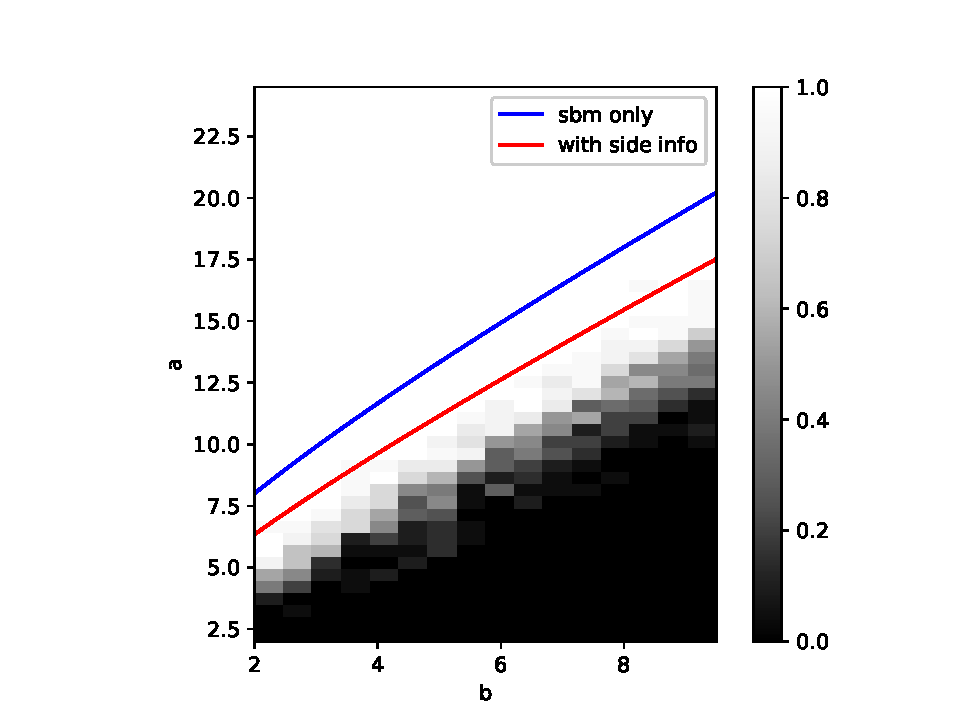
\includegraphics[width=0.8\textwidth]{new_results.pdf}
        \caption{有无额外信息的分界线与SDP算法恢复性能的比较}
        \label{fig:my_label}
    \end{figure}

\section{本章小结}
本章研究了带有额外信息的随机块模型(SBMSI)的精确恢复问题。
具体来说,在给出了 SSBMI 的定义后, 
我们首先针对两社群的情形获得了精确恢复的误差衰减速率。
该结果
表明恢复误差可解耦为由额外信息的雷尼散度和
随机块模型的参数两部分,
从而可以分别进行优化。
另一方面,为
控制恢复误差在给定的允许范围内,
式\eqref{eq:positive_condition_new}
给出了图节点数量和额外信息采样数量所需满足的条件。
而关于为获得误差率所做的假设 \eqref{eq:oneC} 是否可以进一步放宽
这一问题有待于进一步研究。

其次,基于半正定规划(SDP)的数学模型
我们还提出了一个实现 SBMSI 精确恢复的算法。
随着图规模的增大,该算法的恢复误差以多项式的速率收敛到零。
能否将SDP恢复算法拓展到多个社群的情形(有额外信息)目前是一个有
研究价值的开放问题。

\chapter{总结与展望}\label{chp:summary}
\section{工作归纳}
本文在信息论度量应用到社团发现领域的已有工作基础上,
从普适信息论和随机图建模两种思路入手,
建立了信息论度量和社团发现问题在理论分析和算法设计两个层面的联系。
具体来说,本文的工作可总结为以下三部分:

首先,在社团的层次化发现问题上,我们基于多变量互信息对层次化发现问题
进行理论建模,证明了弱独立的随机变量的多变量互信息的计算可以化为一个社团发现问题,
并由此提出了用聚类树表示的层次化结构,与已有的主划分序列PSP算法建立了联系。
进一步地,我们提出了一种高效的层次化发现计算策略——HPSP算法。
该算法的时间复杂度比求解主划分序列的现有算法低一个数量级,
从而可在中等规模的网络中进行社团的层次结构探测。
我们基于多变量互信息的理论,也对异常值检测问题进行了相关的算法设计和实验验证。
该异常值检测算法在未知异常值点数量、含有多个类别的数据集问题上具有应用潜力。

其次,在统计物理启发的社团发现算法方面,我们采用了随机块模型对网络进行建模,
研究了基于玻茨模型的算法
达到精确恢复的条件。我们的结果表明,玻茨模型在随机块模型的社团发现
问题中存在相变现象,在可达到精确恢复的区域内,我们给出了算法误差衰减速率的上界,
并建立了该速率与大偏差理论中速率函数的联系。
进一步地,我们揭示了基于玻茨模型的算法与能量最小化算法、最小割算法、
最大似然算法、最大模块度算法的联系,并比较了它们的误差衰减速率的上界。
该方面的研究为算法分析提供了统一的分析框架,并给出了相关算法误差率的理论保证。

最后,在有辅助信息的社团发现问题上,我们基于雷尼散度研究了有辅助信息的随机块模型,
给出了该模型实现精确恢复的充要条件,并推导了最优误差衰减率的理论极限。
该结果定量地刻画了节点辅助信息和网络中边的信息各自对恢复问题的贡献,
对于指导辅助信息采样数量的选取具有重要意义。
在此基础上,我们设计了半正定规划算法,可满足精确恢复的要求。
在不同参数设定下的实验结果进一步验证了半正定规划算法在有辅助信息的社团发现问题上的有效性。

%本文的工作在社团发现领域具有重要的应用价值。
   %\begin{figure}[!ht]
%    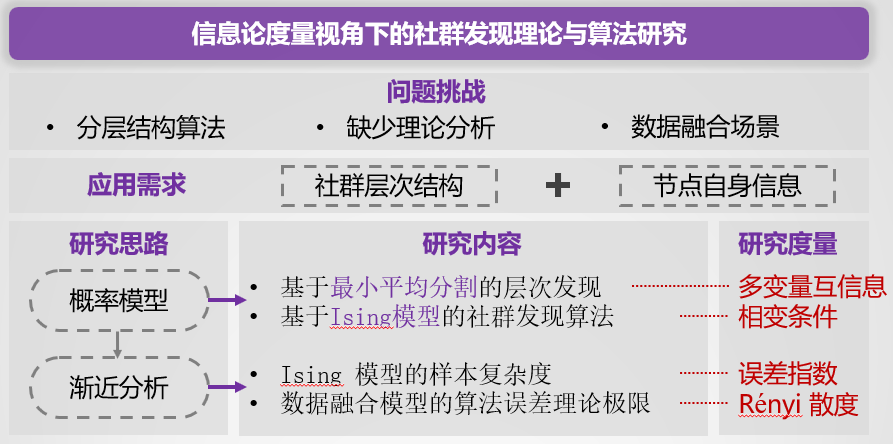
\includegraphics[width=0.9\linewidth]{screenshot-20230130-193759.png}
%\end{figure}

\section{分析技术评注}
本文综合运用了多种信息论
度量研究社团发现问题。
它们均是针对
概率分布的距离度量,可总结为下表:
\begin{table}[!ht]
    \centering
  \begin{tabular}{ccp{8cm}}
    \hline
     度量名称    &   参数个数 &   分布类型 \\
    \hline
     多变量互信息 &    $\geq 2$ &    弱独立的随机变量  \\
     速率函数     &    1 &     两个二项分布的随机变量的差  \\
     雷尼散度     &    2 &    泊松分布和字母集有限的离散型随机变量 \\
    \hline
  \end{tabular}
  \caption{信息论度量的对象}\label{tab:info_metric}
\end{table}

除以上信息论度量外,本文还综合运用了在信息论与统计学的交叉研究领域中的大偏差理论和假设检验问题的研究成果。
在技术证明中,用到了分治法、优化中的对偶理论以及概率统计的相关结论。

信息论度量的分析方法有赖于相关假设的引入,比如
网络由对称的随机块模型生成、辅助信息由离散分布生成等假设。这些假设
是数学中对实际问题建模的一种简化,引入它们的目的是为了
定量地考察算法或模型的性质,使得信息论度量的分析工具的引入成为可能。
需要指出的是,实际网络中网络结构与随机块模型的统计特征不尽相同,
辅助信息也往往不满足理想的假设条件,但这并不影响基于信息论度量分析方法本身的重要性和有效性。

\section{研究展望}
本文的研究可在多方面进行拓展。

在算法设计层面,由于实际处理的图的规模可能比较大,
仿照文献 \inlinecite{faysal2021parallel} 中对 Infomap 这一社团发现算法并行化的思路,
我们可以考虑将本文所研究的HPSP算法和梅特罗波利斯算法并行化。
而在研究玻茨模型的相变性质层面,仿照文献\inlinecite{ye2020exact}的思路,
我们可以从分布\eqref{eq:isingma}独立采集多个
样本,通过系综学习(如多数同意规则)的方式进行社团发现,
然后研究相变点$\beta$和样本数的关系。

此外,本文研究的是带有辅助信息的两社团随机块模型,
该研究思路有望拓展到其他随机图模型或多社团随机块模型上,并
通过似然函数构建类似\eqref{eq:matrix_mle}式
的优化目标,从而指导
一般性的有辅助信息的网络中社团发现的
算法设计。然后我们可以将该方法与通过其他准则\cite{chunaev2020community}构建的算法进行
比较,探索其适用场景。

另一方面,本文的研究聚焦于建立信息论度量与传统社团发现算法的联系。
随着深度学习技术的兴起,社团发现任务亦可藉以
神经网络模型完成\cite{Su_2022},
尤其是在有辅助信息的场景下 \cite{cao2018incorporating}。
仿照本文研究梅特罗波利斯算法、半正定方法的思路,
未来可研究基于神经网络的社团发现方法在随机块模型上的恢复误差
与可解释性等问题。

% 其他部分
\backmatter

% 参考文献
\bibliography{ref/refs}  % 参考文献使用 BibTeX 编译
% \printbibliography       % 参考文献使用 BibLaTeX 编译

% 附录
\appendix
% % !TeX root = ../thuthesis-example.tex

\begin{survey}
\label{cha:survey}

\title{Title of the Survey}
\maketitle


\tableofcontents


本科生的外文资料调研阅读报告。


\section{Figures and Tables}

\subsection{Figures}

An example figure in appendix (Figure~\ref{fig:appendix-survey-figure}).

\begin{figure}
  \centering
  \includegraphics[width=0.6\linewidth]{example-image-a.pdf}
  \caption{Example figure in appendix}
  \label{fig:appendix-survey-figure}
\end{figure}


\subsection{Tables}

An example table in appendix (Table~\ref{tab:appendix-survey-table}).

\begin{table}
  \centering
  \caption{Example table in appendix}
  \begin{tabular}{ll}
    \toprule
    File name       & Description                                         \\
    \midrule
    thuthesis.dtx   & The source file including documentaion and comments \\
    thuthesis.cls   & The template file                                   \\
    thuthesis-*.bst & BibTeX styles                                       \\
    thuthesis-*.bbx & BibLaTeX styles for bibliographies                  \\
    thuthesis-*.cbx & BibLaTeX styles for citations                       \\
    \bottomrule
  \end{tabular}
  \label{tab:appendix-survey-table}
\end{table}


\section{Equations}

An example equation in appendix (Equation~\eqref{eq:appendix-survey-equation}).
\begin{equation}
  \frac{1}{2 \uppi \symup{i}} \int_\gamma f = \sum_{k=1}^m n(\gamma; a_k) \mathscr{R}(f; a_k)
  \label{eq:appendix-survey-equation}
\end{equation}


\section{Citations}

Example citations in appendix.
\cite{abrahams99tex}
\cite{salomon1995advanced}
\cite{abrahams99tex,salomon1995advanced}


\bibliographystyle{unsrtnat}
\bibliography{ref/appendix}

\end{survey}
       % 本科生:外文资料的调研阅读报告
% % !TeX root = ../thuthesis-example.tex

\begin{translation}
\label{cha:translation}

\title{书面翻译题目}
\maketitle

\tableofcontents


本科生的外文资料书面翻译。


\section{图表示例}

\subsection{图}

附录中的图片示例(图~\ref{fig:appendix-translation-figure})。

\begin{figure}
  \centering
  \includegraphics[width=0.6\linewidth]{example-image-a.pdf}
  \caption{附录中的图片示例}
  \label{fig:appendix-translation-figure}
\end{figure}


\subsection{表格}

附录中的表格示例(表~\ref{tab:appendix-translation-table})。

\begin{table}
  \centering
  \caption{附录中的表格示例}
  \begin{tabular}{ll}
    \toprule
    文件名          & 描述                         \\
    \midrule
    thuthesis.dtx   & 模板的源文件,包括文档和注释 \\
    thuthesis.cls   & 模板文件                     \\
    thuthesis-*.bst & BibTeX 参考文献表样式文件    \\
    thuthesis-*.bbx & BibLaTeX 参考文献表样式文件  \\
    thuthesis-*.cbx & BibLaTeX 引用样式文件        \\
    \bottomrule
  \end{tabular}
  \label{tab:appendix-translation-table}
\end{table}


\section{数学公式}

附录中的数学公式示例(公式\eqref{eq:appendix-translation-equation})。
\begin{equation}
  \frac{1}{2 \uppi \symup{i}} \int_\gamma f = \sum_{k=1}^m n(\gamma; a_k) \mathscr{R}(f; a_k)
  \label{eq:appendix-translation-equation}
\end{equation}


\section{文献引用}

文献引用示例\cite{abrahams99tex}。


% 书面翻译的参考文献
\bibliographystyle{unsrtnat}
\bibliography{ref/appendix}

% 书面翻译对应的原文索引
\begin{translation-index}
  \nocite{salomon1995advanced}
  \bibliographystyle{unsrtnat}
  \bibliography{ref/appendix}
\end{translation-index}

\end{translation}
  % 本科生:外文资料的书面翻译
%
\section{定理证明}

%附录是与论文内容密切相关、但编入正文又影响整篇论文编排的条理和逻辑性的资料,例如某些重要的数据表格、计算程序、统计表等,是论文主体的补充内容,可根据需要设置。
\subsection{定理 \ref{thm:weak_independence_equivalent} 的证明}
\begin{proof}[定理 \ref{thm:weak_independence_equivalent} 的证明]
  由$\epsilon$邻域的定义 \ref{def:eps_neighborhood} ,
  $P_{Y|X=x}(y) = P_Y(y) + \sqrt{P_Y(y)}\phi_{Y|X=x}(y)
  \epsilon$。令$\phi_{XY}(x,y)=\sqrt{P_X(x)}\phi_{Y|X=x}(y)$,
  则有
  $P_{XY}(x,y) = P_X(x)P_Y(y) + \sqrt{P_X(x)}\sqrt{P_Y(y)}\phi_{XY}(x,y)
  \epsilon$。
  假设$x\in \mathcal{X}$ 且 $y\in \mathcal{Y}$,
  $\mathcal{X}, \mathcal{Y}$ 均为有限的字母集。
  $\phi_{XY}$ 是 $|\mathcal{X}| \times |\mathcal{Y}|$
  的矩阵,其秩为 $r$。$\phi_{XY}$可以通过奇异值分解的形式写成
  $\frac{1}{r}\sum_{i=1}^r \phi_i \psi^T_i$,其中$\phi, \psi$
  是长度分别为$|\mathcal{X}|, |\mathcal{Y}|$的
  列向量。构造 $U$ 是$[2r]$ 上的均匀分布。
  而$Z_1, Z_2$ 做如下构造:
  \begin{align*}
    P(Z_1=x|U=i) &= P_X(x) + (-1)^i\sqrt{P_X(x)}\phi_{\lceil i/2 \rceil}(x) \sqrt{\epsilon}, x \in \mathcal{X} \\
    P(Z_2=y|U=i) &= P_Y(y) + (-1)^i\sqrt{P_Y(y)}\psi_{\lceil i/2 \rceil}(y) \sqrt{\epsilon}, y \in \mathcal{Y}
  \end{align*}
  $Z_1 | U$ 与$Z_2 | U$ 独立,因此,
  $Z_1, Z_2$ 的联合分布为:
  \begin{align*}
  P(Z_1=x, Z_2=y)& =\sum_{i=1}^{2r}P(U=i)P(Z_1=x|U=i)P(Z_2=y|U=i)\\
  &=P_X(x)P_Y(y) + \sqrt{P_X(x)}\sqrt{P_Y(y)}\frac{\epsilon}{r}
  \sum_{i=1}^{r}\phi_i(x)
  \psi(y) =P(X=x,Y=y)
  \end{align*}
  故$Z_1, Z_2$与$X,Y$具有相同的分布。
  从而不难验证$(Z_1, Z_2)|U$在$(Z_1, Z_2)$的$\sqrt{\epsilon}$邻域内,
  故结论得证。
  \end{proof}

\subsection{定理 \ref{thm:DPX} 的证明}

\begin{lemma}\label{lem:xyz}
	若 $(X,Y)$ 与 $Z$ $\epsilon$-弱独立,
  则 $X$ 与 $Z$ $\epsilon$-弱独立。
\end{lemma}
\begin{proof}
	由两随机变量$\epsilon$-弱独立的定义 \ref{def:weak_indepedent} ,
  我们有
	\begin{equation}\label{eq:pxy_eps}
	P_{X,Y|Z=z}(x,y) = P_{X,Y}(x,y)\left(1+\epsilon \frac{\phi_z(x,y)}{\sqrt{P_{X,Y}(x,y)}}
  \right), z \in \mathcal{Z}
	\end{equation}
	对式\eqref{eq:pxy_eps} 关于 $y\in \mathcal{Y}$ 求和我们有
	\begin{equation}
	P_{X|Z=z}(x) = P_X(x)\left(1+\epsilon\frac{\tilde{\phi}_z(x)}{\sqrt{P_X(x)}} \right),
	\textrm{ 其中 } \tilde{\phi}_z(x) = \frac{\sum_{y\in \mathcal{Y}} \sqrt{P_{X,Y}(x,y) }\phi_z(x,y)}{\sqrt{P_X(x)}}
	\end{equation}
	由 柯西不等式,
  $||\tilde{\phi}_z(x)||^2 \leq \frac{1}{P_X(x)}
	\sum_{y\in \mathcal{Y}}(P_{X,Y}(x,y))
	\sum_{y\in \mathcal{Y}} \phi_z^2(x,y) \leq 1
	$,
	从而推出 $X$  与 $Z$ 弱独立。
\end{proof}
\begin{proof}[定理 \ref{thm:DPX} 的证明]
  由多个随机变量弱独立的定义式 \ref{def:general} ,
  我们可以找到 一个在字母集 $[K]$上的
  离散分布 $U$, 使得 $Z_1, \dots, Z_n$
  关于 $U$ 条件独立。不失一般性,我们假设
  $(Z_1, \dots, Z_n)$ $\epsilon^n$-弱独立。
  则 $(Z_1, \dots, Z_n)$ 和 $U$ $\epsilon$-弱独立,
  由引理 \ref{lem:xyz}  可得 $Z_i$
  和 $U$ $\epsilon$-弱独立,也即有 
\begin{equation}\label{XUk}
P_{Z_i | U=k}(z) = P_{Z_i} (z) \left( 1 + \epsilon {\phi^{(k,i)}(z) \over \sqrt{P_{Z_i}(z)}} \right)
\end{equation}
利用条件分布独立有
\begin{align}
P_{Z_i, Z_j | U = k}(z_i, z_j)
=& P_{Z_i | U=k}(z_i)
P_{Z_j | U=k}(z_j) \notag \\
=& P_{Z_i}(z_i)P_{Z_j}(z_j)
\left(1 + \epsilon
\left(\frac{\phi^{(k,i)}(z_i)}{\sqrt{P_{Z_i}(z_i)}}
+ \frac{\phi^{(k,j)}(z_j)}{\sqrt{P_{Z_j}(z_j)}}
\right) +
\epsilon^2\frac{\phi^{(k,i)}(z_i)
	\phi^{(k,j)}(z_j)}{\sqrt{P_{Z_i}(z_i)P_{Z_j}(z_j)}}
  \right)
  \label{eq:XiXj}
\end{align}
又因为
\begin{align*}
P_{Z_i}(z) &= \sum_{k=1}^{K} P_{Z_i | U=k}(z) P_U(u_k) \\
& =  \sum_{k=1}^{K}P_U(u_k)P_{Z_i} (z)
\left( 1 + \epsilon {\phi^{(k,i)}(z) \over \sqrt{P_{Z_i}(z)}} 
\right) \textrm{ 根据 } \eqref{XUk}\\
\Rightarrow & \sum_{k=1}^{K} P_U(u_k){\phi^{(k, i)}(z) \over \sqrt{P_{Z_i}(z)}} =0,\forall i, z\in \mathcal{Z}
\end{align*}
因此 \eqref{eq:XiXj} 化简为
\begin{equation}\label{eq:PXiXj}
P_{Z_i, Z_j}(z_i, z_j) = P_{Z_i}(z_i)
P_{Z_j}(z_j) \left(
  1+\epsilon^2 \sum_{k=1}^K P_U(u_k)
\frac{\phi^{(k,i)}(z_i)
	\phi^{(k,j)}(z_j)}{\sqrt{P_{Z_i}(z_i)P_{Z_j}(z_j)}}
  \right)
\end{equation}
对于2个以上的随机变量:
\begin{align*}
P_{Z_1,\dots,Z_n}(z_1,\dots,z_n)  &= \sum_{k=1}^{K} P_{Z_1,\dots,Z_n | U=k}(z_1,\dots,z_n) P_U(u_k) \\
&=  \sum_{k=1}^{K}P_U(u_k) \prod_{i=1}^n P_{Z_i|U=k}(z_i)\\
&= \sum_{k=1}^{K} P_U(u_k)\prod_{i=1}^n \left(P_{Z_i} (z_i)( 1 + \epsilon {\phi^{(k,i)}(z_i ) \over \sqrt{P_{Z_i}(z_i)}} )\right)\\
&=  \sum_{k=1}^{K}P_U(u_k) (\prod_{i=1}^n  P_{Z_i} (z_i))
\left( 1 + \epsilon\sum_{i=1}^n {\phi^{(k,i)}(z_i) \over \sqrt{P_{Z_i}(z_i)}} + \epsilon^2\sum_{i\neq j}{\phi^{(k,i)}(z_i)\phi^{(k,j)}(z_j)\over \sqrt{P_{Z_i}(z_i)P_{Z_j}(z_j)} }\right)+o(\epsilon^2) \\
&= (\prod_{i=1}^n  P_{Z_i} (z_i))
\Big(1+\epsilon\sum_{i=1}^n \sum_{k=1}^{K} P_U(u_k){\phi^{(k,i)}(z_i) \over \sqrt{P_{Z_i}(z_i)}} \\
&+\epsilon^2 \sum_{k=1}^{K} P_U(u_k)\sum_{i\neq j}{\phi^{(k,i)}(z_i)\phi^{(k,j)}(z_j)\over \sqrt{P_{Z_i}(z_i)P_{Z_j}(z_j)} } 
\Big) + o(\epsilon^2)\\
&= (\prod_{i=1}^n  P_{Z_i} (z_i))
\left(1 +\epsilon^2\sum_{i\neq j} \sum_{k=1}^{K}P_U(u_k){\phi^{(k,i)}(z_i)\phi^{(k,j)}(z_j)\over \sqrt{P_{Z_i}(z_i)P_{Z_j}(z_j)} }\right) + o(\epsilon^2)
\end{align*}
由 \eqref{eq:PXiXj},
令 $B_{ij}(z_i, z_j)={P_{Z_i, Z_j}(z_i,z_j) - P_{Z_i}(z_i)P_{Z_j}(z_j) \over \sqrt{P_{Z_i}(z_i)P_{Z_j}(z_j)}} $ 可得:
\begin{align}
\epsilon^2\sum_{k=1}^{K}P_U(u_k)
{\phi^{k,i}(z_i)\phi^{k,j}(z_j)\over \sqrt{P_{Z_i}(z_i)P_{Z_j}(z_j)} } & = {P_{Z_i, Z_j}(z_i, z_j) - P_{Z_i}(z_i)P_{Z_j}(z_j) \over P_{Z_i}(z_i)P_{Z_j}(z_j)} \notag\\
& = {B_{ij}(z_i, z_j) \over \sqrt{P_{Z_i}(z_i)P_{Z_j}(z_j)} } \label{eq:Bsecond}
\end{align}
因此,我们有
\begin{equation}\label{eq:sep}
P_{Z_1,\dots,Z_n}(z_1,\dots,z_n) =  (\prod_{i=1}^n  P_{Z_i} (z_i))\left( 1 + \sum_{i\neq j}{B_{ij}(z_i, z_j) \over \sqrt{P_{Z_i}(z_i)P_{Z_j}(z_j)} }\right) +o(\epsilon^2)
\end{equation}
因此 $P_{Z_1,\dots, Z_n}$ 在 $P_{Z_1}\dots P_{Z_n}$ 的
$\epsilon$ 邻域内,且特征函数是
$$\phi(z_1,\dots, z_n)=
\sqrt{P_{Z_1}(z_1)\dots P_{Z_n}(z_n)}
\left(\sum_{i\neq j}{B_{ij}(z_i, z_j) 
\over \sqrt{P_{Z_i}(z_i)P_{Z_j}(z_j)} }\right)
+o(\epsilon^2)$$

由 信息几何的结论,式\eqref{eq:approx:ig} 可得
\begin{align*}
D(P_{Z_1,\dots, Z_n}|| P_{Z_1}\dots P_{Z_n}) & ={1 \over 2} \sum_{z_1,\dots,z_n}\phi^2(z_1,\dots, z_n) \\
& = {1\over 2}\sum_{z_1,\dots,z_n} (\prod_{i=1}^n  P_{Z_i} (z_i)) \left(\sum_{i\neq j}{B_{ij}(z_i, z_j) \over \sqrt{P_{Z_i}(z_i)P_{Z_j}(z_j)} }\right)^2 +o(\epsilon^2) 
\end{align*}
由 $B_{ij}$
的定义式 \eqref{eq:Ixy},
上式可化为对 $\norm{B_{ij}}^2_F$
的求和(平方和中的交叉项外面再求和得零)。
因此,对于分割$\P=\{\{i\}|i\in V\}$ 我们得到
\begin{equation}
D(P_{Z_1,\dots, Z_n}|| P_{Z_1}\dots P_{Z_n}) =   {1 \over 2} \sum_{i\neq j} \norm{B_{ij}}^2_F + o(\epsilon^2)
\end{equation}
对于任意的分割 $\P$,$C\in \P$,
由式\eqref{eq:sep}可得
\begin{equation}
P_{Z_C}(z_C) = \prod_{i\in C} P_{Z_i}(z_i)
\left(1 + \epsilon^2 \sum_{i\neq j,i,j\in C} \frac{B_{ij}(z_i, z_j)}{\sqrt{P_{Z_i}(z_i)P_{Z_j}(z_j)}}
\right) + o(\epsilon^2)
\end{equation}
将上式相乘可得:
\begin{equation}
\prod_{C\in \P}P_{Z_C}(z_C) = \prod_{i=1}^n P_{Z_i}(z_i)
\left(1+\epsilon^2 \sum_{C\in\P}\sum_{i\neq j,i,j\in C}\frac{B_{ij}(z_i, z_j)}{\sqrt{P_{Z_i}(z_i)P_{Z_j}(z_j)}}
\right) + o(\epsilon^2)
\end{equation}
所以 $\prod_{C\in \P}P_{Z_C}$ 在 $P_{Z_1}\dots P_{Z_n}$ 的$\epsilon$ 邻域内,
且 $$\phi_{\P}(z_1,\dots, z_n)=
\sqrt{P_{Z_1}(z_1)\dots P_{Z_n}(z_n)}\left(\sum_{C\in\P}\sum_{i\neq j,i,j\in C}\frac{B_{ij}(z_i, z_j)}{\sqrt{P_{Z_i}(z_i)P_{Z_j}(z_j)}}\right)+o(\epsilon^2)$$
最后,由  \eqref{eq:approx:ig} 得:
\begin{align*}
D(P_{Z_1,\dots, Z_n}|| \prod_{C\in \P}P_{Z_C}) & ={1 \over 2} \sum_{z_1,\dots,z_n}(\phi(z_1,\dots, z_n)-\phi_{\P}(z_1, \dots, z_n))^2 \\
& = {1\over 2}\sum_{z_1,\dots,z_n} \prod_{i=1}^n  P_{Z_i} (z_i) \left(\sum_{\substack{(i,j) \not\in C\\ C\in \P}} {B_{ij}(z_i, z_j) \over \sqrt{P_{Z_i}(z_i)P_{Z_j}(z_j)} }\right)^2 +o(\epsilon^2) \\
& = \frac{1}{2} \sum_{\substack{(i,j) \not\in C\\ C\in \P}} \norm{B_{ij}}_F^2 + o(\epsilon^2)
\end{align*}
从而得到式\eqref{eq:PXV}。
\end{proof}



\subsection{定理 \ref{thm:alg_complexity} 的证明}
\begin{proof}[定理 \ref{thm:alg_complexity} 的证明]
  令
  $\mu_i = \frac{n_i}{n} \leq \frac{1}{2}$。
  下面我们使用数学归纳法证明
  $T(n) = O(n^4)$。
  更具体地,我们将证明 
  $T(n) \leq q C n^4$, 其中 $ q = \frac{16}{5}$。
  $T(3)$ 是一个常数,我们取$C$使得 $T(3)= q C\times 3^4$。
  下面假设
	$T(m) \leq qC m^4$
  对所有 $m \leq n-1$ 成立。
  然后 对于 $T(n)$,
	我们首先证明下式成立:
	\begin{equation}\label{eq:outerI}
	\sum_{i=1}^k T(n_i) \leq 10 T\left(\frac{n}{2}\right)
	\end{equation}
	因为 $\sum_{i=1}^k T(n_i) \leq qC n^4\sum_{i=1}^k u_i^4$ 并且
  从式 \eqref{eq:Tn} 中可得
  $10 T\left(\frac{n}{2}\right) \geq 10Cn^4 
  \left(\frac{1}{2}\right)^4$。根据
	\begin{equation}\label{eq:innerI}
       q\sum_{i=1}^k u_i^4 \leq 10 \left(\frac{1}{2}\right)^4 
	\end{equation}
	我们有 \eqref{eq:innerI} $\Rightarrow$ \eqref{eq:outerI}。
  由定理 \ref{thm:alg_complexity} 中的条件,
  我们不妨假设
  $u_1\leq u_2 \leq \dots \leq u_k \leq \frac{1}{2}$
  且 $\sum_{i=1}^k u_i = 1$。
  因此,我们有
  $u_1 \leq \frac{1}{k}, u_2 \leq \frac{1}{k-1}, \dots, u_{k-1} \leq \frac{1}{2}$。
	根据
  \begin{equation}\label{eq:outerOne}
	 q \left[2 \left(\frac{1}{2}\right)^4 + \sum_{i=3}^k \left(\frac{1}{i}\right)^4\right]
   \leq 10  \left(\frac{1}{2}\right)^4
	\end{equation}
	我们有 \eqref{eq:outerOne} $\Rightarrow$ \eqref{eq:innerI}。
  并且代入$q=\frac{16}{5}$,
  \eqref{eq:outerOne} 等价于
	$\sum_{i=3}^k \left(\frac{1}{i} \right)^4 \leq \frac{9}{8}\left(\frac{1}{2}\right)^4$。
  进一步地,
	\begin{align*}
		\sum_{i=3}^k \left(\frac{1}{i} \right)^4 & < \frac{1}{9}\sum_{i=3}^k \left(\frac{1}{i}
    \right)^2 \\
		& < \frac{1}{9}\sum_{i=3}^k \frac{1}{i(i-1)} \\
		& < \frac{1}{18}
    < \frac{9}{8}\left(\frac{1}{2}
    \right)^4
	\end{align*}
	因此,
  式 \eqref{eq:outerI} 成立。然后
  由 式\eqref{eq:Tn} 和 $T(k) \leq T\left(\frac{n}{2}\right)$ 可得
	\begin{align}
		T(n)  & \leq Cn^4 + 11T\left(\frac{n}{2} \right) \\
		& \leq C n^4 + 11 q C \left(\frac{n}{2}\right)^4
    = \frac{16}{5} C n^4
	\end{align}
\end{proof}

\subsection{定理 \ref{thm:triangle} 的证明}
首先我们证明如下引理:
\begin{lemma}\label{thm:trival}
  分割 $\P_k = \{\{1\},\{2\},\dots,\{\abs{V}\}\}$ 
  使得 $\frac{f[\P]}{\abs{\P}-1}$
  最小 当且仅当 式\eqref{eq:GFP} 成立。
  \begin{equation}\label{eq:GFP}
  \frac{f[\P]}{\abs{\P}-1} \geq \frac{f[\P_k]}{\abs{V}-1} \textrm{ 对于任何 } \P \in \Pi'
  \end{equation}
  \end{lemma}
  \begin{proof}
  由文献\inlinecite{narayanan}中的定理3可知,
  定义在式\eqref{eq:hlambda}中的$h(\lambda)$ 是分段线性函数,
  $h(\lambda)$ 的第一段
  是 $ - \lambda $ 且 
  最后一段是 $ f[\P_k] - \abs{V} \lambda$。
  它们的交点是
  $(\lambda_{+}, -\lambda_{+})$,
  其中
  $\lambda_{+} = \frac{f[\P_k]}{\abs{V}-1}$。
  因为 $\frac{f[\P]}{\abs{\P}-1} \geq \lambda_{+} \iff f[\P] - \abs{\P}\lambda_{+} \geq - \lambda_{+}$,
  式 \eqref{eq:GFP}
  相当于说 $h(\lambda)$ 在 $\lambda = \lambda_{+}$
  的最小值点是
  $\{V\}$ 或
  $\{\{1\},\{2\},\dots,\{\abs{V}\}\}$
  并且 $h(\lambda)$ 只有两段。
  从几何的观点来看,$\min\frac{f[\P]}{\abs{\P}-1}$
  是 $h(\lambda)$ 第一个分界点,
  该分界点与$h(\lambda)$最后一个分界点
  相等 当且仅当 \eqref{eq:GFP} 成立。
  \end{proof}
  \begin{proof}[定理 \ref{thm:triangle} 的证明]
    我们将使用归纳法证明对于任意的分割$\P \in \Pi$,
    式\eqref{eq:GF} 成立。
    \begin{equation}\label{eq:GF}
    f[\P] \geq \frac{\abs{\P}-1}{\abs{V}-1} \sum_{(i,j) \in E} w_{ij}
    \end{equation}
    
    然后由引理 \ref{thm:trival} 
    即可得证。
    
    设 $n=\abs{V}$。
    若 $\abs{\P}=n$,
    易得式 \eqref{eq:GF} 取等号。
    
    假设 式\eqref{eq:GF} 对 任意
    $\abs{\P} \geq k+1(k\geq 2)$成立,
    下面我们讨论 $\P=\{C_1, \dots, C_k\}$
    的情形。
    因为$\P$是非平凡的分割,
    因此存在某个$\abs{C_i}\geq 2$。
    不妨设$\abs{C_1}=n_1\geq 2$,
    构造$\P$的一个细分$\P'$如下:
    $\P_{C_1} = \{\{i\}| i \in C_1\}, \P'=\P_{C_1} \cup \P \backslash \{C_1\}$。
    则我们有 $\abs{\P'} = k+n_1-1$。
    对$\P'$运用 式\eqref{eq:GFP} 有
    \begin{align}\label{eq:PPrelation}
    f[\P'] &
    \geq \frac{k+n_1 -2}{n-1}\sum_{(i,j) \in E} w_{ij} \\
    f[\P] & =f[P'] - \sum_{(i,j) \in E(C_1)} w_{ij}
    \end{align}
    其中
    $E(C_1) =\{ (i,j) |i<j, i, j\in C_1 \}$。
    对任意$k \not\in C_1$运用三角不等式
    $w_{ij} \leq w_{ik} + w_{jk}$,
    并关于所有 $i, j \in C_1, i\neq j$求和,
    我们有
    $$
    \sum_{(i,j) \in E(C_1)} w_{ij} \leq \sum_{(i,j) \in E(C_1)} (w_{ik} + w_{jk}) = (n_1-1)\sum_{i\in C_1} w_{ik}
    $$
    再将上式对所有 $k \not\in C_1$ 求和
    $$
    (n - n_1) \sum_{(i,j) \in E(C_1)} w_{ij} \leq (n_1 - 1) \sum_{i \in C_1, k \not\in C_1} w_{ik}
    $$
    另外,注意到
    \begin{align*}
    \sum_{(i,j) \in E} w_{ij}  & \geq \sum_{(i,j) \in E(C_1)} w_{ij} + \sum_{i\in C_1, k\not\in C_1} w_{ik} \\
    (n_1 - 1)\sum_{(i,j) \in E} w_{ij}  & \geq (n_1 -1 )\sum_{(i,j) \in E(C_1)} w_{ij} + (n_1-1)\sum_{i\in C_1, k\not\in C_1} w_{ik} \\
    & \geq (n_1 -1 )\sum_{(i,j) \in E(C_1)} w_{ij} + (n - n_1) \sum_{(i,j) \in E(C_1)} w_{ij}\\
    & = (n-1) \sum_{(i,j) \in E(C_1)} w_{ij}
    \end{align*}
   因此我们得到 $\sum_{(i,j) \in E(C_1)} w_{ij} \leq \frac{n_1-1}{n-1}\sum_{(i,j) \in E} w_{ij}$。
   从式 \eqref{eq:PPrelation} 可得
    $f[\P] \geq \frac{k-1}{n-1}\sum_{(i,j) \in E} w_{ij}$。
    因此,结论对 $\abs{\P}=k$ 成立。
    \end{proof}
\subsection{定理 \ref{thm:main_N} 的证明}
    \begin{proof}[定理 \ref{thm:main_N} 的证明]
      设 $V' = B \cup \{i'\}$。我们首先做出如下的符号约定:
      $w(C) = \displaystyle\sum_{(i,j) \in E(C)} w_{ij},$
      $w(A, C) = \displaystyle\sum_{\substack{i \in A, j \in C \\ (i,j) \in E(V')}} (w_{ij}+w_{ji})$ 且
      $\P_C = \{\{i \}| i \in C \}$。
      假设 $\gamma_N = I(Z_B)$,
      由式 \eqref{eq:largest_threshold} 可得
      $\gamma_N =\frac{f[\P_B]} {\abs{B} -1}$。
      此外,我们有
      $f[\P_{V'}] = f[\P_B] + \sum_{i \in B}w_{ii'}$。
      
      若 $ \sum_{i \in B} w_{ij} > \gamma_N$, 我们可得
      $$
      \gamma'_N \geq I_{\P_{V'}}(Z_{V'}) = \frac{(\abs{B}-1)\gamma_N
      + \sum_{i \in B}w_{ii'}}{\abs{B}} > \gamma_N
      $$
      
      另一方面, 假设 
      $\gamma'_N = I(Z_K) > \gamma_N$,
      则 $K$ 必包含 $i'$。
      若 $K=V'$, 则结论成立。
      否则, 假设 $K = \{i'\} \cup B', B=B'\cup J, J\neq \emptyset$,
      则我们有
      \begin{equation}\label{eq:gammaNF}
      \gamma_N = \frac{w(J,B') + w(J) + w(B')}{ \abs{B'} + \abs{J} - 1 }
      \end{equation}
      因为 $I(Z_K) = I_{\P_K}(Z_K)$ 是最大的,
      我们有 $I_{\P_K}(Z_K) > I_{\P_{V'}}(Z_{V'})$ 且
      $I_{\P_K}(Z_K) \geq I_{\P_{B'}}(Z_{B'})$。
      \begin{align*}
      \frac{w(\{i'\}, B') + w(B')}{\abs{B'}} >& \frac{w(B') + w(J, B') + w(J) + w(\{i'\}, B') + w(\{i'\}, J)}{\abs{B'} + \abs{J}}  \\
      \frac{w(\{i'\}, B') + w(B')}{\abs{B'}} \geq & \frac{w(B')}{\abs{B'} - 1}
      \end{align*}
      于是可得
      \begin{align}
      \abs{J} \left(w(\{i'\}, B') + w(B') \right) > &
      \abs{B'} \left(w(J, B') + w(J) + w(\{i'\}, J) \right)
      \label{eq:target}
      \\
      (\abs{B'} - 1)  w(\{i'\}, B') \geq & w(B') \label{eq:convert}
      \end{align}
      将 式\eqref{eq:convert} 代入 式\eqref{eq:target} 可得
      \begin{equation}\label{eq:summation}
      \abs{J} w(\{i'\}, B') > w(J, B') + w(J) + w(\{i'\}, J)
      \end{equation}
      结合 式\eqref{eq:gammaNF},
      将 式\eqref{eq:convert} 与 式\eqref{eq:summation} 相加我们可得
      $w(\{i'\}, B') > \gamma_N$。
      所以 $\sum_{j \in B}w_{ii'} > \gamma_N $ 成立。
    \end{proof}
  

%% !TeX root = ../thuthesis-example.tex
\section{定理证明}
\subsection{定理\ref{thm:ab12} 的证明}
\begin{lemma}\label{lem:ER_tr_counting}
  \newglossaryentry{e_r}{name=埃尔德什-雷尼模型, description={Erdős–Rényi model}}
  考虑一个由\gls{e_r}生成的随机图 $G$,它有  $n$
  个节点, 每条边以概率 $p$ 随机生成\cite{erdHos1960evolution}。
   假设
	$p=\A$, 边的数量
  记为  $N_E$ 
  而图中三角形的
  数量记为  $T$。 则
  \newglossaryentry{not:converge_in_probability}
{
  type=notation,
  name={$\xrightarrow{p}$},
  description={随机变量的依概率收敛}
}
	$\frac{N_E}{n \log n} \xrightarrow{p} \frac{a}{2}$ 且
  $\frac{T}{\log^3 n} \xrightarrow{p} \frac{a^3}{6}$。
  这里, 符号 $\xrightarrow{p}$ 表示\glsdesc{not:converge_in_probability}。
\end{lemma}
\begin{proof}
		令 $X_{ij}$ 表示
    参数 为 $p$ 的伯努利随机变量。
    \newacronym{acr:iid}{i.i.d.}{Independent and identically distributed}
    则 $N_E
    = \sum_{i,j} X_{ij}$, $X_{ij}$ 是 \gls{acr:iid}
    的随机变量。
	$\mathbb{E}[N_E] = \frac{n(n-1)}{2}p = \frac{(n-1)\log n}{2}a$ 
  且  $\Var[N_E] = \frac{n(n-1)}{2} p(1-p) < a\frac{(n-1)\log n}{2}$。
	则由切比雪夫不等式,
	\begin{align*}
	P(\Big|\frac{N_E}{n \log n } - \frac{a}{2} \frac{n-1}{n}\Big| > \epsilon) & \leq
	\frac{1}{\epsilon^2}\Var \left[\frac{N_E } {n \log n } \right] \\
	& < \frac{a(n-1)}{2n^2\epsilon^2\log n}
	\end{align*}
	
	对于给定的 $\epsilon$, 当 $n$ 充分大时,
  \begin{align*}
	P \left(\Big|\frac{N_E}{n \log n } - \frac{a}{2} \Big| > \epsilon \right) & <
	P \left(\Big|\frac{N_E}{n \log n } - \frac{a}{2} \frac{n-1}{n}\Big| > 2\epsilon \right) \\
	& \leq \frac{n-1}{8n^2 \epsilon^2 \log n}
	\end{align*}
	
	因此, 由依概率收敛的定义
  我们有 $\frac{N_E}{n \log n} \xrightarrow{p} \frac{a}{2}$。
	
	令 $X_{ijk}$ 表示参数为  $p^3$ 的 Bernoulli 随机变量。
	则 $T = \sum_{i,j,k} X_{ijk}$。
	易得 $\mathbb{E}[T] = \binom{n}{3}p^3$。
  因为 $X_{ijk}$ 并不独立,
  不能直接用独立同分布的公式计算 $T$ 的方差。
	由  \citet{holland1977method} 一文可知:
	% Mordern version: https://stats.stackexchange.com/questions/338267/distribution-and-variance-of-count-of-triangles-in-random-graph
	\begin{align*}
	\Var[T]  &= \binom{n}{3} p^3 + 12 \binom{n}{4} p^5 + 30 \binom{n}{5} p^6 + 20 \binom{n}{6} p^6
	 - \binom{n}{3}^2 p^6  \\ 
   &= O(\log^3 n)
	\end{align*}
	
	因此
	由 切比雪夫不等式可得
	\begin{align*}
	P \left (\Big|\frac{T}{\log^3 n } - \frac{a^3}{6} \frac{(n-1)(n-2)}{n^2}\Big| > \epsilon \right)
   &\leq \frac{1}{\epsilon^2} \Var[ \frac{T}{\log^3 n} ]\\ 
	& = \frac{1}{\epsilon^2}O \left(\frac{1}{\log^3 n} \right)
	\end{align*}
	    
	从而得到 $\frac{T}{\log^3 n} \xrightarrow{p} \frac{a^3}{6}$。
\end{proof}
因为每条边的生成是独立的,埃尔德什-雷尼模型中的
$N_E$ 的收敛性 %define if appropriate.
可以直接拓展到
随机块模型。
但是对于三角形的数量$T$,因为每个三角形存在与否并不独立,事情变得棘手。
下面的两个引理给出了随机块模型中的三角形个数的方差的公式。
\begin{lemma}\label{lem:SBM_tr_counting_cross}
	考虑 $\SSBM(2n, 2, p, q)$。它有两个
  社团,记为 $S_1$ 和 $S_2$。
    计算三角形的个数 $T$, 并且这些三角形
    有一个顶点在  $S_1$ 中,
    该顶点对应的边在 $S_2$中。
   则 $T$ 的方差为:
\begin{align}
\Var[T]  = \frac{n^2(n-1)}{2}pq^2 + n^2(n-1)(n-2)p^2q^3 
 + \frac{n^2(n-1)^2}{2}pq^4 - \frac{n^2(n-1)(3n-4)}{2} p^2 q^4
 \label{eq:SBM_tr_counting_cross}
\end{align}
\end{lemma}
\begin{proof}
	由定义, $T=\sum_{i,j,k} Y_{ijk}$,
  其中 $i,j,k$三个点之间两两有边相连时 $Y_{ijk}$ 取值为1,否则为0。
  这里的求和是
  针对 所有 的 $i \in S_1$ 和 $j,k \in S_2$。
  因此, $\E[T] = n\binom{n}{2}pq^2$。
	为计算 $T$ 我们需要求出 $\E[T^2] = \sum_{i,j,k}\sum_{i',j',k'} Y_{ijk}Y_{i'j'k'}$。
	根据三元组 $(i,j,k)$ 和 $(i',j',k')$ 重合的情况
  $\E[Y_{ijk}Y_{i'j'k'}]$的值一共有6种不同的情形:
	\begin{enumerate}
		\item $\{i,j,k\} = \{i',j',k'\}$,则 $E[Y_{ijk}Y_{i'j'k'}] = pq^2$。
		在 $\E[T^2]$的求和式中共有 $n\binom{n}{2}$ 
     项。以下五种情形均需考虑$\E[T^2]$ 中出现的2倍的系数。
		\item 若 $\{i,j,k\}$ 和 $\{i',j',k'\}$ 只有
    一个共同的元素
    并且这个元素在 $ S_1$ 中, 则 $\E[Y_{ijk}Y_{i'j'k'}] = p^2q^4$。
		在 $\E[T^2]$的求和式中共有 $6n\binom{n}{4}$ 项 ($\binom{4}{2}=6$ )。
		\item 若 $\{i,j,k\}$ 和 $\{i',j',k'\}$ 只有一个共同的元素
    并且这个元素 在 $ S_2$ 中,则
    $E[Y_{ijk}Y_{i'j'k'}] = p^2q^4$。在 $\E[T^2]$的求和式
		中共有 $12\binom{n}{2}\binom{n}{3}$ 项。
		\item 若 $\{i,j,k\}$ 和 $\{i',j',k'\}$ 恰有 2  个 共同的元素
    并且这两个元素均在 $S_2$ 中,
    则 $E[Y_{ijk}Y_{i'j'k'}] = pq^4$。
    在 $\E[T^2]$的求和式
		中共有  $2\binom{n}{2}\binom{n}{2}$ 项。
\item 若 $\{i,j,k\}$ 和 $\{i',j',k'\}$ 恰有2  个 共同的元素
且一个在 $S_1$ 中,另一个在 $S_2$ 中,则 $E[Y_{ijk}Y_{i'j'k'}] = p^2q^3$。
在 $\E[T^2]$的求和式
		中共有 $6n\binom{n}{3}$ 项。
\item  若 $\{i,j,k\}$ 和 $\{i',j',k'\}$ 没有共同的元素,
 则 $E[Y_{ijk}Y_{i'j'k'}] = p^2q^4$。
 在 $\E[T^2]$的求和式中共有 $12\binom{n}{2}\binom{n}{4}$ 
 项。
	\end{enumerate}
通过下面的求和式可以验证我们已经遍历了所有的情形:
% Mathematica Code:
% Simplify[n^2 (n-1)/2 + 12 Binomial[n,2] Binomial[n,3] + 6 n Binomial[n,4] + Binomial[n,4] Binomial[n,2]*12 + 6 n Binomial[n,3]+ 2 Binomial[n,2]^2]
\begin{equation}\label{eq:ver_nn2}
  n\binom{n}{2} + 6n\binom{n}{4} + 12\binom{n}{2} \binom{n}{3} + 2\binom{n}{2}^2 + 6n\binom{n}{3} + 12\binom{n}{2}\binom{n}{4} = \left(n\binom{n}{2}\right)^2  
\end{equation}
\eqref{eq:ver_nn2}式右端中出现的$n\binom{n}{2}$ 是$\E[T] $ 中求和式的项数。
\end{proof}
\begin{lemma}\label{lem:SBM_tr_counting_3}
	考虑 $\SSBM(3n, 3, p, q)$。它有3个社团,记为
  $S_1,S_2$ 和 $S_3$。
  计算三角形的个数 $T$,
  并且这些三角形 有一个顶点在$S_1$中,有一个顶点在 $S_2$中,
  有一个顶点在 $S_3$ 中。
	则 $T$ 的方差为:
	\begin{equation*}\label{eq:SBM_tr_counting_three}
	\Var[T] = n^3 q^3  + 3n^3(n-1) q^4  + 3 n^3 (n-1)^2 q^5 - n^3(3n^2-3n+1)q^6
	\end{equation*}
\end{lemma}

\begin{proof}
	与引理\ref{lem:SBM_tr_counting_cross} 的证明类似,
	$\E[T] = n^3 q^3$,对于$\E[T^2]$求和式中的项共如下4种情形:
	\begin{enumerate}
	\item 若 $\{i,j,k\} = \{i',j',k'\}$, 则 $E[Y_{ijk}Y_{i'j'k'}] = q^3$。
	$\E[T^2]$中 共有 $n^3$ 项。
	\item 若 $\{i,j,k\}$ 和 $\{i',j',k'\}$ 有一个共同的元素, 则 $E[Y_{ijk}Y_{i'j'k'}] = q^5$。
	$\E[T^2]$中 共有 $12n\binom{n}{2}^2$ 项。
	\item 若 $\{i,j,k\}$ and $\{i',j',k'\}$ 有两个共同的元素, 则 $E[Y_{ijk}Y_{i'j'k'}] = q^4$。
	$\E[T^2]$中 共有 $6\binom{n}{2}n^2$ 项。
	\item If $\{i,j,k\}$ and $\{i',j',k'\}$ 没有共同的元素, 则  $E[Y_{ijk}Y_{i'j'k'}] = q^6$。
	$\E[T^2]$中 共有 $8\binom{n}{2}^3$ 项。
\end{enumerate}	
通过下面的求和式可以验证我们已经遍历了所有的情形:
$$
6\binom{n}{2}n^2  + 8\binom{n}{2}^3 + 12n\binom{n}{2}^2 +  n^3 = n^6
$$
\end{proof}
\begin{lemma}\label{lem:sbmV}
 对于 $\SSBM(n, k, p, q)$,其中 $p=\frac{a\log n}{n}, q = \frac{b\log n}{n}$。
 三角形的数量为 $T$。
	则 $\frac{T}{(\log n)^3}$ 依概率收敛到 $\frac{1}{k^2}(\frac{a^3}{6} + \frac{k-1}{2}ab^2 + (k-1)(k-2)\frac{b^3}{6} )$。
\end{lemma}
\begin{proof}
 我们将 $T$ 分成三部分:
 第一部分是每个社团内部的三角形,记社团$i$里有$T_i$个三角形,则共有$k$个$T_i$的项。
 第二部分包括有一个点在第i个社团内部,它所对的边在第$j$个社团里的那些三角形,记为 $T_{ij}$。
 共有 $k(k-1)$ 个 $T_{ij}$ 的项。第三部分包括三个顶点分别在$i,j,k$三个不同社团的三角形,共有
 $\binom{n}{3}$ 项。
	
	我们只需证明:
\begin{align}
	\frac{T_i}{\log ^3 n} &\xrightarrow{p} \frac{(a/k)^3}{6} \\
	\frac{T_{ij}}{\log^3 n}& \xrightarrow{p}\frac{1}{2}(a/k)(b/k)^2\\
	\frac{T_{ijk}}{\log^3 n} & \xrightarrow{p} (b/k)^3
	\end{align}
	
	$\frac{T_i}{\log ^3 n}$ 的收敛性可以直接从引理
 \ref{lem:ER_tr_counting} 中得到。这里,我们视$p=\frac{(a/k) (
    \log (n/k) + \log k)}{(n/k)}$,因为 $\log k$ 相比于其前一项量阶更小,
    可以忽略不计。
	对于 $T_{ij}$, 我们使用 
  引理\ref{lem:SBM_tr_counting_cross} 的结果。
	在 \eqref{eq:SBM_tr_counting_cross} 式中
  我们用 $n/k$ 代替 $n$, 取 $p=a\frac{\log n}{n}$ 且 $q=b\frac{\log n}{n}$。
	$\Var[T_{ij}] \sim \frac{ab^2}{2k^3} \log^3 n$。
  因为 $\frac{T_{ij}}{\log^3 n}$ 的期望值是
  $(n/k)\binom{n/k}{2}pq^2/(\log^3 n)
	=\frac{n-1}{2n}\frac{ab^2}{k^3}$, 由切比雪夫不等式
  可得:
	\begin{align*}
	P \left( \Big|\frac{T_{ij}}{\log^3 n} - \frac{n-1}{2n}\frac{ab^2}{k^3} \Big| > \epsilon
  \right) &\leq \frac{\Var[T_{ij} / \log^3 n]}{\epsilon^2} \\
	& = \frac{1}{\epsilon^2}
	O \left( \frac{1}{\log^3 n} \right)
	\end{align*}
	
	因此, $\frac{T_{ij}}{\log^3 n} $ 依概率收敛到 $\frac{1}{2}(a/k)(b/k)^2$。
	
	为证明
  $\frac{T_{ijk}}{\log^3 n}\to (b/k)^3$,
  从 引理\ref{lem:SBM_tr_counting_3} 中
  可得 $\Var[T_{ijk}] = O(\log^5 n)$:
	$$
	P \left( \Big|\frac{T_{ijk}}{\log^3 n} -\frac{b^3}{k^3} \Big| > \epsilon
  \right) \leq \frac{\Var[T_{ijk} / \log^3 n]}{\epsilon^2} = \frac{1}{\epsilon^2}
	O \left(\frac{1}{\log n} \right)
	$$
\end{proof}
\begin{proof}[定理\ref{thm:ab12} 的证明]
	令 $e^*_1 = \frac{a+(k-1)b}{2k}$, $k^2 e^*_2 = \frac{a^3}{6} + \frac{k-1}{2}ab^2 + (k-1)(k-2)\frac{b^3}{6}$
	且 $e_1 = \frac{T_1}{n\log n}, e_2 = \frac{T_2}{\log^3 n}$。
	由 引理
 \ref{lem:ER_tr_counting}, $e_1 \to e^*_1$。
	由 引理\ref{lem:sbmV}, 当 $n\to \infty$ 时,
  $e_2 \to e^*_2$。
	通过变量替换 $x=2ke_1 - (k-1)y$ 消元,我们可将
  方程组 (\ref{eq:e_1},\ref{eq:e_2})
  化简为如下的非线性方程:
\begin{equation}\label{eq:gy_y3}
g(y): = (k-1)(y^3 - 6 e_1 y^2 + 12 e_1^2 y) + 6 e_2 - 8 k e_1^3 = 0
\end{equation}

$g'(y) = 3(k-1)(y-2e_1)^2 \geq 0 $,
$g(y)$ $\mathbb{R}$上的是增函数,
因此方程\eqref{eq:gy_y3} 最多有一个实根。
下面我们证明\eqref{eq:gy_y3}式有一个实根
在 区间 $(0, 2e_1)$ 内。
\begin{align*}
&\lim_{n\to \infty}g(0) =  6e^*_2 - 8k(e^*_1)^3 =-\frac{3}{k^2}(k-1)(k-2)ab^2 \\
&-\frac{3(k-1)}{k^2}a^2b - \frac{k-1}{k^2} ((k-2)-(k-1)^2)b^3 < 0 \\
&\lim_{n\to \infty}g(2e_1) = 6e^*_2 - 8(e^*_1)^3 = \frac{(k-1)(a-b)^3}{k^3} > 0
% verified with sympy
\end{align*}

因此,\eqref{eq:gy_y3}式有一个实根,由 $g(y)$的连续性,当$n\to \infty $ 时,该实根收敛到 $b$。
从而我们得到方程组 (\ref{eq:e_1},\ref{eq:e_2})有唯一解 $\hat{a},\hat{b}$,
且
$\hat{b} \to b$, $\hat{a} \to a$。
\end{proof}

\subsection{引理\ref{lem:lemmaDiff}的证明}

\begin{proof}[引理\ref{lem:lemmaDiff}的证明]
	首先我们将
  \eqref{eq:energy} 式改写成
	\begin{equation*}
	H(\bar{\sigma}) = \gamma \frac{\log n}{n} \sum_{i < j} \delta(\bar{\sigma}_i, \bar{\sigma}_j)
	- (1 + \gamma\frac{\log n}{n}) \sum_{ \{i, j\} \in E(G)} \delta(\bar{\sigma}_i, \bar{\sigma}_j)
	\end{equation*}
	
	接着我们逐步计算能量差:
  \begin{align*}
	H(\bar{\sigma}') - H(\bar{\sigma}) =& 
  \left(1 + \gamma\frac{\log n}{n}
  \right)
  \cdot \sum_{i \in N_r(G)} (\delta(\bar{\sigma}_r, \bar{\sigma}_i) -
	\delta(\omega^s \cdot \bar{\sigma}_r, \bar{\sigma}_i)) \\
	&+ \gamma \frac{\log n}{n}\sum_{i\neq r}
	( \delta(\omega^s \cdot \bar{\sigma}_r, \bar{\sigma}_i) -
	\delta( \bar{\sigma}_r, \bar{\sigma}_i) ) \\
	 =& \left(
     1 + \gamma\frac{\log n}{n}
     \right)
   \sum_{i \in N_r(G)} J_s(\bar{\sigma}_r, \bar{\sigma}_i) \\
	&+ \gamma \frac{\log n}{n}\sum_{i=1}^n
	( \delta(\omega^s \cdot \bar{\sigma}_r, \bar{\sigma}_i) -
	\delta( \bar{\sigma}_r, \bar{\sigma}_i) +1) \\
	=& \left(1+\gamma \frac{\log n}{n}
  \right)
  \sum_{i \in N_r(G)} J_s(\bar{\sigma}_r, \bar{\sigma}_i)\\
	&+ \gamma \frac{\log n}{n} (m(\omega^s \cdot \bar{\sigma}_r)-m(\bar{\sigma}_r)+1)
	\end{align*}
\end{proof}

\subsection{定理\ref{thm:phase_transition}的证明}
\label{sec:appendix_theorem_proof_phase_trans}

在开始定理\ref{thm:phase_transition}的技术证明之前,
我们需要介绍一些辅助的
符号。

% Some additional notation is needed for the proof.
注释\ref{re:energy_diff}中指出了
$X$改变一个状态后的能量差表达式。
对于一般的情形,即改变
$|\cI|:=\Dist(\bar{\sigma}, X)$
个位置的状态后,
我们可以将能量差写成:
\begin{equation}\label{eq:Hgeneral}
H(\bar{\sigma}) - H(X)=
(1 + \gamma \frac{ \log n}{n})[A_{\bar{\sigma}} - B_{\bar{\sigma}}] + \gamma\frac{ \log n}{n} N_{\bar{\sigma}}
\end{equation}
在上式中 我们使用
$A_{\bar{\sigma}}$ 或
$B_{\bar{\sigma}}$ 来表示
服从参数分别为 $\A$ 或 $\B$ 的二项分布的随机变量,并且
$N_{\bar{\sigma}}$ 是一个依赖于 $\bar{\sigma}$ 但与图结构无关的非随机的正整数。
引理\ref{lem:minus} 给出了 $A_{\bar{\sigma}}, B_{\bar{\sigma}}$ 和 $N_{\bar{\sigma}}$
的表达式:

\begin{lemma}\label{lem:minus}
	对于 $\SSBM(n,k,p,q)$,
  我们假设 $\bar{\sigma}$ 
  在总共$|\cI|:=\Dist(\bar{\sigma}, X)$ 
  个坐标位置上不同于真值标签向量
  $X$。
	对于 $i\neq j$,令 $I_{ij} = \Big|\{r\in [n] \big| X_r = w^i, \sigma_r = w^j \}\Big|$
  且 $I_{ii} = 0$。
  我们进一步将行和$I_i$
  和列和$I'_i$分别表示为:
  \begin{align}
  I_i &= \frac{n}{k} -
  \Big|\{r\in [n] \big| X_r = w^i, \sigma_r=w^i \}\Big|
  =
  \sum_{j=0}^{k-1} I_{ij} \label{eq:I_i_horizontal} \\
  I'_i &=
  \Big|\{r\in [n] \big| X_r \neq w^i,
  \sigma_r=w^i \}\Big|
  =\sum_{j=0}^{k-1} I_{ji}\label{eq:I_prime_i_vertical}
  \end{align}
	则
\begin{align}
	N_{\bar{\sigma}} &= \frac{1}{2}\sum_{i=0}^{k-1} (I_i - I_i')^2 \label{eq:N_w} \\
	B_{\bar{\sigma}} & \sim \Binom(N_{B_{\bar{\sigma}}} , q),
  N_{B_{\bar{\sigma}}}=\frac{n}{k}|\cI| + \frac{1}{2}\sum_{i=0}^{k-1}  (-2 I'_i I_i  + I'^2_i - \sum_{j=0}^{k-1} I^2_{ji})
  \label{eq:B_w}\\
	A_{\bar{\sigma}} &
  \sim \Binom(N_{A_{\bar{\sigma}}}, p),
  N_{A_{\bar{\sigma}}}=
  \frac{n}{k}|\cI| - \frac{1}{2}\sum_{i=0}^{k-1}
   (I^2_i + \sum_{j=0}^{k-1} I^2_{ij})
  \label{eq:A_w}
	\end{align}
\end{lemma}
\begin{proof}
  由式\eqref{eq:isingma}、\eqref{eq:energy}可得
	\begin{align}
  \log P_{\sigma|G}(\sigma=\bar{\sigma})
  & = 
  \beta(1 + \frac{\gamma \log n}{n}) \sum_{\{i,j\} \in E(G)}  \delta(\bar{\sigma}_i, \bar{\sigma}_j)  
	- \beta\frac{\gamma \log n}{n} \sum_{1\leq i<j \leq n} \delta(\bar{\sigma}_i, \bar{\sigma}_j)  - \log Z_G(\beta, \gamma)
  \notag\\
  & = 
  \beta(1 + \frac{\gamma \log n}{n}) \sum_{\bar{\sigma}_i = \bar{\sigma}_j} Z_{ij}
	- \beta\frac{\gamma \log n}{n}
  \sum_{\bar{\sigma}_i = \bar{\sigma}_j} 1 
  - \log Z_G(\beta, \gamma)
  \label{eq:log_P_sigma_G_bar_sigma}
  \end{align}
	其中 $Z_{ij}$ 服从伯努利分布,
  $P(Z_{ij}=1)$ 等于节点$i$与节点$j$之间有边相边的概率。
	对于 $\sigma = X$, 我们有
	\begin{align}
	\sum_{X_i = X_j} Z_{ij} &
  = \sum_{X_i = X_j, \bar{\sigma}_i = \bar{\sigma}_j}
  Z_{ij} + \sum_{X_i = X_j, \bar{\sigma}_i \neq \bar{\sigma}_j}
  Z_{ij}
  \label{eq:split_zij_tmp_X_ij}\\
	\sum_{X_i = X_j} 1 &= \frac{1}{2} \sum_{i=0}^{k-1} \frac{n}{k} 
  \left( \frac{n}{k} - 1 
  \right)\label{eq:split_one_tmp_X_ij}
	\end{align}
	对于 $\sigma = \bar{\sigma}$,我们有
	\begin{align}
	\sum_{\bar{\sigma}_i = \bar{\sigma}_j} Z_{ij} &= \sum_{X_i = X_j, \bar{\sigma}_i = \bar{\sigma}_j} Z_{ij} + \sum_{X_i \neq X_j, \bar{\sigma}_i = \bar{\sigma}_j} Z_{ij} 
  \label{eq:split_zij_tmp_sigma_ij}\\
	\sum_{\bar{\sigma}_i = \bar{\sigma}_j} 1 &= \frac{1}{2} \sum_{i=0}^{k-1} (I'_i + \frac{n}{k} - I_i) ( I'_i + \frac{n}{k} - I_i - 1)
  \label{eq:split_one_tmp_sigma_ij}
	\end{align}
  其中,式 \eqref{eq:split_one_tmp_sigma_ij} 是根据式
  \eqref{eq:I_i_horizontal}和 \eqref{eq:I_prime_i_vertical}
  而来。
	注意到
  $
  \Big|\{r\in [n] \big| X_r = w^i, \sigma_r=w^i \}\Big|
  =\frac{n}{k} - I_i$和
	$|\{r\in [n] | X_r \neq \omega^i, \sigma_r = \omega^i \}| = I'_i$,
	我们因此有  
  \begin{equation}\label{eq:number_of_sigma_r_equal_omega_i}
    |\{r\in [n] | \sigma_r = \omega^i \}|
    = I'_i + \frac{n}{k} - I_i
  \end{equation}
  类比式\eqref{eq:split_one_tmp_X_ij}从而得到
  式\eqref{eq:split_one_tmp_sigma_ij}。

  由式\eqref{eq:Pratio} 我们得到
  \begin{equation}
    \frac{P_{\sigma |G } (\sigma = \bar{\sigma})}
    {P_{\sigma |G } (\sigma = X)}
    = \exp(-\beta(H(\bar{\sigma})
    - H(X)))
  \end{equation}
  结合式\eqref{eq:log_P_sigma_G_bar_sigma}
  可得
  \begin{equation}\label{eq:Hgeneral_tmp_derived}
    H(\bar{\sigma}) - H(X)=
    -\left(1 + \gamma \frac{ \log n}{n}
    \right)
    \left[
      \sum_{\bar{\sigma}_i = \bar{\sigma}_j}Z_{ij} - \sum_{X_i = X_j}Z_{ij}
      \right]
    + \gamma\frac{ \log n}{n}
    \left[\sum_{\bar{\sigma}_i = \bar{\sigma}_j}1 - \sum_{X_i = X_j}1
    \right]
    \end{equation}
  将式\eqref{eq:Hgeneral_tmp_derived} 与式\eqref{eq:Hgeneral}
  对比可得:
  \begin{align}
    B_{\bar{\sigma}} - A_{\bar{\sigma}} &=
    \sum_{\bar{\sigma}_i = \bar{\sigma}_j}Z_{ij}
    - \sum_{X_i = X_j}Z_{ij}
    \label{eq:B_bar_A_bar_lem_minus}\\
    N_{\bar{\sigma}} &=
    \sum_{\bar{\sigma}_i = \bar{\sigma}_j} 1  -\sum_{X_i = X_j} 1
    \label{eq:N_bar_sigma_lem_minus}
  \end{align}
  由式\eqref{eq:split_one_tmp_X_ij},
  \eqref{eq:split_one_tmp_sigma_ij}, 
  \eqref{eq:N_bar_sigma_lem_minus} 可得
  $N_{\bar{\sigma}} = \sum_{\bar{\sigma}_i = \bar{\sigma}_j} 1  -\sum_{X_i = X_j} 1 = \frac{1}{2}\sum_{i=0}^{k-1} (I_i - I_i')^2 $,
  即式 \eqref{eq:N_w}。
	另一方面,由式\eqref{eq:B_bar_A_bar_lem_minus},
  \eqref{eq:split_zij_tmp_X_ij}, 
  \eqref{eq:split_zij_tmp_sigma_ij}
  可得 $B_{\bar{\sigma}} - A_{\bar{\sigma}} = \sum_{X_i \neq X_j, \bar{\sigma}_i = \bar{\sigma}_j} Z_{ij} - \sum_{X_i = X_j, \bar{\sigma}_i \neq \bar{\sigma}_j} Z_{ij}$。
	对于在求和式 $\sum_{X_i \neq X_j, \bar{\sigma}_i = \bar{\sigma}_j} Z_{ij}$
  中出现的 $Z_{ij}$, $Z_{ij} \sim \Bern(q)$
  并且我们有
  \begin{align}
  \sum_{X_i \neq X_j, \bar{\sigma}_i = \bar{\sigma}_j} 1 
  &= \sum_{i=0}^{k-1}[(\frac{n}{k} - I_i) I_i' + \frac{1}{2} \sum_{j=0}^{k-1} I_{ji}(I'_i - I_{ji}) ] 
  \label{eq:x_i_neq_x_j_bar_sigma_i_eq_bar_sigma_j_0}\\
	&=\frac{n}{k}|\cI| + \frac{1}{2}\sum_{i=0}^{k-1}  (-2 I'_i I_i  + I'^2_i - \sum_{j=0}^{k-1} I^2_{ji}) 
  \label{eq:x_i_neq_x_j_bar_sigma_i_eq_bar_sigma_j_1}
  \end{align}
  在式\eqref{eq:x_i_neq_x_j_bar_sigma_i_eq_bar_sigma_j_0}
  最外层的求和中,首先遍历的是$X_i=1, \omega, \dots, \omega^{k-1}$。  
  而式\eqref{eq:split_one_tmp_sigma_ij}
  利用了
  $|\cI| = \sum_{i=0}^{k-1} I'_i$。
  类似的,
  对于在求和式 $\sum_{X_i = X_j, \bar{\sigma}_i \neq \bar{\sigma}_j} Z_{ij}$
  中出现的 $Z_{ij}$, $Z_{ij} \sim \Bern(p)$。
	$\sum_{X_i = X_j, \bar{\sigma}_i \neq \bar{\sigma}_j} 1
	= \sum_{i=0}^{k-1}[(\frac{n}{k} - I_i) I_i + \frac{1}{2} \sum_{j=0}^{k-1} I_{ij}(I_i - I_{ij}) ] 
	= \frac{n}{k}|\cI| - \frac{1}{2}\sum_{i=0}^{k-1}  (I^2_i + \sum_{j=0}^{k-1} I^2_{ij})$。
  从而式\eqref{eq:B_w}、\eqref{eq:A_w} 得证。
\end{proof}

从上面可以看到引理\ref{lem:minus} 的证明并没有很多技巧性,主要涉及一些计数
的技巧。
当 $|\cI|$ 相比与 $n$ 很小时
我们有如下的引理, 该引理是 \citet{ye2020exact} 中 陈述 6 的拓展。 

\begin{lemma}
  \label{lem:enhanced_fb}
	对于 $t\in [\frac{1}{k}(b-a), 0], 0<\delta <1$
	和 $ |\cI| \le n/\log^{\delta} n$,我们有
\begin{equation} \label{eq:upmpt}
	P_G(B_{\bar{\sigma}}-A_{\bar{\sigma}}\ge t |\cI| \log n) 
	\le  \exp\Big(|\cI|\log n
	\left(
    f_{\beta}(t) - \beta t -1	+ O((\log n)^{-\delta}) \right)\Big)
	\end{equation}
	其中 $f_{\beta}(t) := \min_{s\geq 0} (g(s) - st) + \beta t \leq \tilde{g}(\beta) $。
  $P_G$中的下标$G$表示图$G$是由SSBM模型随机生成的。
  函数$g(\beta), \tilde{g}(\beta)$
  的定义分别参见
  \eqref{eq:g_beta_main_article}
  和
  \eqref{eq:g_tilde_beta_main_article} 式。
\end{lemma}

在引理\ref{lem:enhanced_fb} 中,
取
$|\cI|=1, N_{\bar{\sigma}}=0$,
此时$A_{\bar{\sigma}} \sim \Binom(\frac{n}{k}, \A),
B_{\bar{\sigma}} \sim \Binom(\frac{n}{k}, \B)$,
即得到 式\eqref{eq:introduction_g_a_b_eps}。

\begin{proof}[引理\ref{lem:enhanced_fb} 的证明]
  由$f_{\beta}(t)$函数的定义,
  \eqref{eq:upmpt}式中
  $f_{\beta}(t) - \beta t$ 与$\beta$无关而只与
  $t$有关。
	由定义可知,
  $A_{\bar{\sigma}}\sim \Binom(N_{A_{\bar{\sigma}}},\frac{a\log n}{n})$
  且
	$B_{\bar{\sigma}}\sim\Binom(N_{B_{\bar{\sigma}}},\frac{b\log n}{n})$,
  并且二者彼此独立。
  由 (\ref{eq:N_w}-\ref{eq:A_w})可知,$N_{B_{\bar{\sigma}}} - N_{A_{\bar{\sigma}}}
  = N_{\bar{\sigma}}$。
  对于$s>0$,
  $B_{\bar{\sigma}}-A_{\bar{\sigma}}$ 的矩生成函数可以展开成
	\begin{align}
	 \mathbb{E}[e^{s(B_{\bar{\sigma}}-A_{\bar{\sigma}})}] 
	& =\Big(1-\frac{b\log n}{n}+\frac{b\log n}{n} e^s \Big)^{N_{B_{\bar{\sigma}}}}
	\Big(1-\frac{a\log n}{n}+\frac{a\log n}{n} e^{-s} \Big)^{N_{A_{\bar{\sigma}}}}  \notag\\
	& = \exp\left(\frac{\log n}{n}\left(N_{B_{\bar{\sigma}}}
  (be^s - b) + N_{A_{\bar{\sigma}}}(ae^{-s}-a) + N_{B_{\bar{\sigma}}}
  O \left(\frac{\log n}{n} \right) \right) \right)
  \label{eq:exp_s_B_A_sigma}
	\end{align}
	由\eqref{eq:B_w}
  和\eqref{eq:A_w}
  注意到$k$是个常数,
  当
  $|\cI| \le n/\log^{\delta}(n)$ 时
	我们能估计
  $N_{B_{\bar{\sigma}}}$和$N_{A_{\bar{\sigma}}}$
  的阶数。它们分别是
  $N_{A_{\bar{\sigma}}} = \frac{n}{k}|\cI| + O(|\cI|^2)$,
	 $N_{B_{\bar{\sigma}}} = \frac{n}{k}|\cI| + O(|\cI|^2)$。
	\begin{align*}
	\mathbb{E}[e^{s(B_{\bar{\sigma}}-A_{\bar{\sigma}})}]
   \le&
	\exp(\frac{\log n}{n}\Big((\frac{n}{k}|\cI| + O(|\cI|^2))(be^s - b) +(\frac{n}{k} |\cI| + O(|\cI|^2))(ae^{-s}-a) \\
  &+ \frac{n}{k}|\cI|O(\frac{\log n}{n}) \Big))\\
	=
  & \exp\Big(\frac{|\cI| \log n}{k}(a e^{-s}+b e^s-a-b +
	O(\log^{-\delta}(n))) \Big),
	\end{align*}
	最后一个等式来自于
  $ |\cI| \le n/\log^{\delta}(n)$这个假设。
	由切尔诺夫不等式(参见 \eqref{eq:chernoff_bound}),
  对于 $s>0$,我们有
	\begin{align*} 
	& P_G(B_{\bar{\sigma}}-A_{\bar{\sigma}}\ge t |\cI| \log n)\le
	\frac{\mathbb{E}[e^{s(B_{\bar{\sigma}}-A_{\bar{\sigma}})}]}{e^{st |\cI|  \log n}}  \\
	\le & \exp\Big(\frac{|\cI|\log n}{k} \big(a e^{-s}+b e^s -kst -a-b
	+ O(\log^{-\delta}(n)) \big)\Big)  .
	\end{align*}
	上式右端对$s\geq 0$取最小值即有
  \eqref{eq:upmpt}。  
	\end{proof}

  对应于定理\ref{thm:phase_transition} 的三种情况,我们需要使用若干个非平凡的引理来辅助证明。

  \begin{lemma}\label{lem:sigmaX}
    令 $\gamma > b$, 且 $\bar{\sigma}$ 满足 $\Dist(\bar{\sigma}, X) \geq \frac{n}{\sqrt{\log n}}$
    和 $D(\bar{\sigma}, X)$
    (参见\eqref{eq:D_sigma_sigma_prime})
    两个条件。
    事件
    $P_{\sigma | G}(\sigma = \bar{\sigma} ) > \exp(-Cn) P_{\sigma | G}(\sigma = X)$
    发生的概率小于 $\exp(-\tau(\beta, \gamma) n \sqrt{\log  n} )$,
    其中 $C$ 是任意事先给定的常数而 
    $\tau(\beta, \gamma)$
   是某个依赖于$\gamma$ 和 $\beta$的取值为正值的函数。
  \end{lemma}
  \begin{proof}
    我们把 事件 $P_{\sigma | G}(\sigma = \bar{\sigma} ) > \exp(-Cn) P_{\sigma | G}(\sigma = X)$
    记为 $\widetilde{D}(\bar{\sigma}, C)$。
    由 \eqref{eq:Hgeneral} 式, $\widetilde{D}(\bar{\sigma}, C)$
    等价于:
  \begin{equation}\label{eq:BwA}
    (1 + \frac{\gamma \log n}{n})[B_{\bar{\sigma}} - A_{\bar{\sigma}}] >  \frac{\gamma \log n}{n} N_{\bar{\sigma}}  - \frac{C}{\beta} n
    \end{equation}  
    
    我们声称$\bar{\sigma}$  必须满足以下两个条件中的至少一个。
    \begin{enumerate}
      \item $\exists i\neq j$ s.t. $\frac{1}{k(k-1)}\frac{n}{\sqrt{\log n}} \leq I_{ij} \leq \frac{n}{k} - \frac{1}{k(k-1)}\frac{n}{\sqrt{\log n}}$
      \item $\exists i \neq j$ s.t. $I_{ij} > \frac{n}{k} - \frac{1}{k(k-1)}\frac{n}{\sqrt{\log n}}$ and $I_{ji} < \frac{1}{k(k-1)}\frac{n}{\sqrt{\log n}}$
    \end{enumerate}
    $I_{ij}$的定义参见引理
   \ref{lem:minus}。
    如果上面两个条件均不成立,则由条件1,对 $0 \leq i,j\leq k-1$,
    我们有
    $I_{ij} < \frac{1}{k(k-1)}\frac{n}{\sqrt{\log n}}$
    或者 $I_{ij} > \frac{n}{k} - \frac{1}{k(k-1)}\frac{n}{\sqrt{\log n}}$。
    
    因为 $\sum_{i,j} I_{ij} = |\cI| \geq \frac{n}{\sqrt{\log n}}$,
    存在 $i,j$ 使得
    $I_{ij} > \frac{n}{k} - \frac{1}{k(k-1)}\frac{n}{\sqrt{\log n}}$.
    对于这一对确定的 $i,j$,不妨先假设 $I_{ji} > \frac{n}{k} - \frac{1}{k(k-1)}\frac{n}{\sqrt{\log n}}$,
    下面我们将推出一对矛盾说明该假设不成立。
    取 $X'$ 为在$X$ 的基础上交换$w^i$ 和 $w^j$ 位置的向量,
    然后我们考虑
  \begin{align}
     \Dist(\bar{\sigma}, X') & - \Dist(\bar{\sigma}, X)= |\{ r \in [n]|X_r=w^i, \bar{\sigma}_r \neq w^j \}| \notag\\
    &+ |\{ r \in [n]|X_r=w^j, \bar{\sigma}_r \neq w^i \}| \notag\\
    &-|\{ r \in [n]|X_r=w^i, \bar{\sigma}_r \neq w^i \}| \notag\\
    &- |\{ r \in [n]|X_r=w^j, \bar{\sigma}_r \neq w^j \}| \notag\\
    & = \frac{n}{k} - I_{ij} +  \frac{n}{k} - I_{ji} - I_i - I_j\label{eq:distsmall} \\
    & < \frac{2}{k(k-1)}\frac{n}{\sqrt{\log n}} - I_i - I_j < 0\notag
    \end{align}
    这和 $\bar{\sigma}$ 离 $X$ 最近的条件矛盾。
    因此
    $I_{ji} > \frac{n}{k} - \frac{1}{k(k-1)}\frac{n}{\sqrt{\log n}}$
    不成立,由条件1
    则有  $I_{ji} < \frac{1}{k(k-1)}\frac{n}{\sqrt{\log n}}$。
    但这样一来 $(i, j)$ 二元组满足 条件 2,
    又与 $\bar{\sigma}$ 不满足如上两个条件的假设相矛盾。
    
    在条件1的假设下,我们能获得 $N_{A_{\bar{\sigma}}}$的一个下界。
    为方便估计该下界,我们首先改写\eqref{eq:A_w}式。
    对于 $i\neq j$ ,令 $I'_{ij} = I_{ij}$,
    而 $I'_{ii} = \frac{n}{k} - I_i$。
    则我们有:
    \begin{align*}
    N_{A_{\bar{\sigma}}} &=
    \frac{n}{k}|\cI| - \frac{1}{2}\sum_{i=0}^{k-1}
    (I^2_i + \sum_{j=0}^{k-1} I^2_{ij}) \\
    &=
    \frac{n}{k}|\cI| - \frac{1}{2}\sum_{i=0}^{k-1}
    ((\frac{n^2}{k^2} - 2\frac{n}{k} I'_{ii}) +
    \sum_{j=0}^{k-1} I'^2_{ij}) \\
    &=
    \frac{n}{k}|\cI| - \frac{1}{2}\sum_{i=0}^{k-1}
    ((\frac{n^2}{k^2} - 2\frac{n}{k} (\frac{n}{k} - I_i)))
    - \frac{1}{2}\sum_{i=0}^{k-1}\sum_{j=0}^{k-1} I'^2_{ij} \\
    &= \frac{n^2}{2k} - \frac{1}{2}
    \sum_{i=0}^{k-1} \sum_{j=0}^{k-1} I'^2_{ij}
   \end{align*}
    
    在求和式中 $\sum_{i=0}^{k-1} \sum_{j=0}^{k-1} I'^2_{ij}$
    的每一项 $\sum_{j=0}^{k-1} I'^2_{ij}$ 其满足 $\sum_{j=0}^{k-1}
    I'_{ij} = \frac{n}{k}$,当某个$I'_{ii}$取$\frac{n}{k}$
    而其余的项为零时$\sum_{j=0}^{k-1} I'^2_{ij}$
    最大。但由于条件1成立,有某一行不能取
    这种极端值,所以 $\sum_{i=0}^{k-1} \sum_{j=0}^{k-1} I'^2_{ij}$中
    共有 $(k-1)$行求和得$ (k-1)\frac{n^2}{k^2}$
    而其中一行则必须保留$I'_{ij}, I'_{ii}$ 这两个非零项。
    因此 $\sum_{i=0}^{k-1} \sum_{j=0}^{k-1} I'^2_{ij}
    \leq (k-1)\frac{n^2}{k^2} + (\frac{n}{k} - I_{ij})^2 + I^2_{ij}$。
    而这里的
    $I_{ij}$ 满足条件1。
    进一步的, $\sum_{i=0}^{k-1} \sum_{j=0}^{k-1} I'^2_{ij} \leq (k-1)\frac{n^2}{k^2} + (\frac{1}{k(k-1)}\frac{n}{\sqrt{\log n}})^2
    + (\frac{n}{k} - \frac{1}{k(k-1)}\frac{n}{\sqrt{\log n}})^2 = \frac{n^2}{k} - \frac{2n^2}{k^2 (k-1)\sqrt{\log n}}(1+o(1))$。
    从而我们得到
  \begin{equation}\label{eq:Asigma}
    A_{\bar{\sigma}} \geq \frac{n^2}{k^2 (k-1)\sqrt{\log n}}(1+o(1))
    \end{equation}
    
    
    在条件2的假设下, 我们能得到
    $N_{\bar{\sigma}}$的一个下界。
    因为
    $\Dist(\bar{\sigma}, X') - \Dist(\bar{\sigma}, X) \geq 0$,
     由 \eqref{eq:distsmall} 式 我们有
    $I_{ij} + I_{ji} + I_{i} + I_j \leq \frac{2n}{k} $。
    又因为 $I_i \geq I_{ij} > \frac{n}{k} - \frac{1}{k(k-1)}\frac{n}{\sqrt{\log n}}$,
    从而$I_j $ 满足
    $I_j \leq \frac{2}{k(k-1)}\frac{n}{\sqrt{\log n} }$。
    进一步有 $I'_j - I_j \geq I_{ij} - I_j \geq  \frac{n}{k} - \frac{3}{k(k-1)}\frac{n}{\sqrt{\log n} }$。
    由 \eqref{eq:N_w}
    式 $N_{\bar{\sigma}} \geq \frac{1}{2}(\frac{n}{k} - \frac{3}{k(k-1)}\frac{n}{\sqrt{\log n}})^2 = \frac{n^2}{2k^2}(1+o(1))$.
    
    下面我们用
     切尔诺夫不等式给出\eqref{eq:BwA}式描述的事件发生概率的上界。
     在分析中我们可以省略不等号左边的 $\frac{\gamma \log n}{n}$ 一项
     ,因为其远小于$1$。
    令 $Z \sim \Bern(\A), Z' \sim \Bern(\B)$,则:
    \begin{align*}
    &P_G(\widetilde{D}(\bar{\sigma}, C))
    \leq (\mathbb{E}[\exp(sZ')])^{N_{B_{\bar{\sigma}}}}
    (\mathbb{E}[\exp(-sZ)])^{N_{A_{\bar{\sigma}}}}\\
    &\cdot \exp(-s(\frac{\gamma \log n}{n} N_{\bar{\sigma}}  - \frac{C}{\beta}n)) \\
    & \leq \exp\Big(N_{B_{\bar{\sigma}}}
    \frac{b\log n}{n}(e^s -1) + N_{A_{\bar{\sigma}}}\frac{a\log n}{n} (e^{-s} - 1) \\
    &-s(\frac{\gamma \log n}{n} N_{\bar{\sigma}}  - \frac{C}{\beta}n)\Big) 
    \end{align*}
    
    使用 $N_{B_{\bar{\sigma}}} = N_{\bar{\sigma}} + N_{A_{\bar{\sigma}}}$
    我们可以进一步简化上式中的指数项为:
    $$
    \frac{\log n}{n} [N_{A_{\bar{\sigma}}}(b(e^s -1)+ a(e^{-s} - 1)) +
    N_{\bar{\sigma}} (b(e^s - 1)-\gamma s)]  + s \frac{C}{\beta}n
    $$
    
    下面我们考察 函数 $g_1(s) = b(e^s -1)+ a(e^{-s} - 1)$
    和 $g_2(s) = b(e^s - 1)-\gamma s$。
    两个函数 在 $s=0$ 处取值为零
    并且 $g_1'(s) = (be^s - ae^{-s}), g_2'(s) = be^s -\gamma$。
    因此, $g_1'(0) = b-a<0, g_2'(0) = b - \gamma < 0$
    我们可以选择 $s^*>0$,使得 $g_1(s^*) < 0,g_2(s^*) < 0$。
    为了补偿 $sCn/\beta$ 这一项的影响,我们只需要确保
    $\frac{\log n}{n} \min\{N_{A_{\bar{\sigma}}}, N_{\bar{\sigma}}\}$ 的阶次大于$n$。
    由于   $N_{A_{\bar{\sigma}}}\geq \frac{n^2}{k^2 (k-1)\sqrt{\log n}}(1+o(1))$ 或 $N_{\bar{\sigma}} \geq \frac{n^2}{2k^2}(1+o(1))$
    有一个成立,
    这一要求可以得到了满足。
  \end{proof}

\begin{lemma}\label{prop:small}
  若 $\gamma>b$, $\beta>\beta^\ast$,
  对于 $1\leq r \leq \frac{n}{\sqrt{\log n}}$
  和 $\forall \epsilon > 0$,
  存在集合 $\cG^{(r)}$ 使得:
\begin{equation}\label{eq:Gr}
  P_G(\cG^{(r)}_n) \ge 1 - n^{r(\tilde{g}(\beta)/2 + \epsilon)}
  \end{equation}
  并且对于任意 $G\in\cG^{(r)}_n$,有
\begin{equation}\label{eq:psigmaX}
  \frac{P_{\sigma|G}(\Dist(\sigma, X)=r | D(\sigma, X))}
  {P_{\sigma|G}(\sigma=X | D(\sigma, X))} <
  n^{r \tilde{g}(\beta) /2}
  \end{equation}
  
  对于 $r> \frac{n}{\sqrt{\log n}}$, 存在集合 $\cG^{(r)}$ 使得:
\begin{equation}\label{eq:Gr1}
  P(G\in\cG^{(r)}_n) \ge 1 - e^{-n}
  \end{equation}
  并且对于任意 $G\in\cG^{(r)}_n$,有
\begin{equation}\label{eq:psigmaX1}
  \frac{P_{\sigma|G}(\Dist(\sigma, X)=r | D(\sigma, X))}
  {P_{\sigma|G}(\sigma=X | D(\sigma, X))} <
  e^{-n}
  \end{equation}
\end{lemma}
\begin{proof}
  我们将讨论分为两种情况: $r\leq \frac{n}{\sqrt{\log n}}$
  和 $r > \frac{n}{\sqrt{\log n}}$。
  
  当 $r\leq \frac{n}{\sqrt{\log n}}$ 时,
  通过使用 关于 $\Dist$
  的三角不等式,
  我们可以证明 
  $\Dist(\sigma, X) = r$ 蕴含
  $D(\sigma, X)$。
   对于 $f \in S_k \backslash \{ \textrm{id} \}$,
   其中
   $\textrm{id}$ 是恒等映射,
   我们有:
  $$
  \frac{2n}{k} \leq \Dist(f(X), X) \leq \Dist(\sigma, f(X)) + \Dist(\sigma, X)
  $$
  
  因此,
  $\Dist(\sigma, f(X)) \geq \frac{2n}{k} - \frac{n}{\sqrt{\log n}} \geq \Dist(\sigma, X)$。
  从而我们得到
  \eqref{eq:psigmaX} 式 等价于:
  \begin{equation}\label{eq:psigmaX2}
  \frac{P_{\sigma|G}(\Dist(\sigma, X)=r)}
  {P_{\sigma|G}(\sigma=X)} <
  n^{r \tilde{g}(\beta) /2}
  \end{equation}
  
  上式左边可以写为:
  \begin{align*}
  \frac{P_{\sigma|G}(\Dist(\sigma, X)=r)}
  {P_{\sigma|G}(\sigma=X)}  &= \sum_{\Dist(\bar{\sigma}, X)=r}\exp(-\beta(H(\bar{\sigma})-H(X)))\\
  \textrm{ by \eqref{eq:Hgeneral} } &\leq \sum_{\Dist(\bar{\sigma}, X)=r}\exp(\beta_n(B_{\bar{\sigma}}-A_{\bar{\sigma}}))
  \end{align*}
  其中 
  \begin{equation}\label{eq:beta_n_def}
  \beta_n = \beta(1+\gamma\frac{\log n}{n})
  \end{equation}
  
  定义
  $\Xi_n(r): = \sum_{\Dist(\bar{\sigma}, X)=r}\exp(\beta_n(B_{\bar{\sigma}}-A_{\bar{\sigma}}))$,
  我们只需证明:
  \begin{equation}
  P_{G}(\Xi_n(r) \geq n^{r \tilde{g}(\beta) /2}) \leq  n^{r (\tilde{g}(\beta) /2 + \epsilon)}
  \end{equation}
  
  定义 事件 $\Lambda_n(G,r):=\{B_{\bar{\sigma}} -A_{\bar{\sigma}} < 0, \forall \bar{\sigma}\, s.t. \Dist(\bar{\sigma}, X)=r\}$,
  然后我们采用下面的方式进行处理
  \begin{align*}
  P_{G}(\Xi_n(r) \geq n^{r \tilde{g}(\beta) /2}) \leq
  P_G(\Lambda_n(G,r)^c)
  + P_G\left(
    \Xi_n(r) \geq n^{r \tilde{g}(\beta) /2} |\Lambda_n(G,r) 
    \right)
  \end{align*}
  
  对于第一项, 因为
  $|\{ \bar{\sigma} | \Dist(\bar{\sigma}, X) = r \}| \leq (k-1)^r n^r$,
  由 引理\ref{lem:enhanced_fb} 可得
  $P_G(\Lambda_n(G,r)^c) \leq (k-1)^r n^{rg(\bar{\beta})} \leq n^{r (\tilde{g}(\beta) /2 + \epsilon/2)}$。

  对于第二项,我们使用马尔可夫不等式:
  \begin{align*}
  P_G(\Xi_n(r) \geq n^{r \tilde{g}(\beta) /2} |\Lambda_n(G,r) )
  \leq \mathbb{E}[\Xi_n(r)|\Lambda_n(G,r)]n^{-r \tilde{g}(\beta) /2} 
  \end{align*}
  
  而上式中的条件期望可以做如下估计:
  \begin{align*}
  &\mathbb{E}[\Xi_n(r)|\Lambda_n(G,r)]=
  \sum_{\Dist(\bar{\sigma}, X) = r}\sum_{tr\log n = -\infty }^{-1} 
   P_G(B_{\bar{\sigma}} -A_{\bar{\sigma}}=tr\log n)\exp(\beta_n tr \log n) \\
  & \leq (k-1)^r n^{r+r\beta_n(b-a)/k} +
  \sum_{\Dist(\bar{\sigma}, X) = r}\sum_{tr\log n = r\frac{b-a}{k}\log n }^{-1} 
   P_G(B_{\bar{\sigma}} -A_{\bar{\sigma}}=tr\log n)\exp(\beta_n tr \log n)
  \end{align*}
  $1+\beta_n(b-a)/k = f_{\beta_n}(\frac{b-a}{k}) < \tilde{g}(\beta_n)$,
  因此,
  $(k-1)^r n^{r+r\beta_n (b-a)/k}n^{-r \tilde{g}(\beta) /2} \leq$
   $n^{r (\tilde{g}(\beta) /2 + \epsilon/2)} $。
  使用 引理\ref{lem:enhanced_fb}, 我们有:
  \begin{align*}
  P_G(B_{\bar{\sigma}} -A_{\bar{\sigma}}=tr\log n)\exp(\beta_n rt \log n) \leq 
  n^{r(f_{\beta_n}(t)-1 + O(\frac{1}{\sqrt{\log n}}))}
  \end{align*}
  
  因为 $\beta_n \to \beta$, $\forall \epsilon$,
  当 $n$ 充分大时
  我们有 $\tilde{g}(\beta_n) \leq \tilde{g}(\beta) + \epsilon /2$。
  因此,
  \begin{align*}
  &n^{-r \tilde{g}(\beta) /2}\sum_{\Dist(\bar{\sigma}, X) = r}\sum_{\substack{tr\log n = \\ r(b-a)/k\log n} }^{-1}
  P_G(B_{\bar{\sigma}} -A_{\bar{\sigma}}=t\log n)\exp(\beta_n rt \log n) \\
  & \leq  (k-1)^r r\frac{b-a}{k} ( \log n )
  n^{r(\tilde{g}(\beta_n) - \tilde{g}(\beta)/2)}\\
  & \leq  n^{r(\tilde{g}(\beta)/2 + \epsilon/2)} O(\log n) (k-1)^r
  \end{align*}
  
  结合上面的式子, 我们可以得到:
  \begin{align*}
  P_{G}(\Xi_n(r) \geq n^{r \tilde{g}(\beta) /2}) &\leq  n^{r(\tilde{g}(\beta)/2 + \epsilon/2)} O(\log n) (k-1)^r\\
  &\leq n^{r(\tilde{g}(\beta)/2 + \epsilon)}
  \end{align*}
  
  当 $r>\frac{n}{\sqrt{\log n}}$时,
  由引理\ref{lem:sigmaX},
  我们选取充分大的常数  $C>1$
  使得 $k^n\exp(-Cn) < e^{-n}$:
  \begin{align*}
  &\frac{P_{\sigma|G}(\Dist(\sigma, X)=r | D(\sigma, X))}
  {P_{\sigma|G}(\sigma=X | D(\sigma, X))} = 
  \sum_{\substack{D(\bar{\sigma}, X) \\ 
  \Dist(\bar{\sigma}, X)=r}} \frac{P_{\sigma | G}(\sigma = \bar{\sigma}) }{P_{\sigma | X}(\sigma = X)} > \exp(-n)\\
  &\Rightarrow \exists \bar{\sigma},
  \frac{P_{\sigma | G}(\sigma = \bar{\sigma}) }{P_{\sigma | X}(\sigma = X)} > k^{-n}\exp(-n)
  \Rightarrow \exists \bar{\sigma},
  \frac{P_{\sigma | G}(\sigma = \bar{\sigma}) }{P_{\sigma | X}(\sigma = X)} > \exp(-Cn)\\
  \end{align*}
  最后一个事件发生的概率小于 $k^ne^{-\tau(\beta, \gamma) n\sqrt{\log n}}<e^{-n}$。
  因此,   \eqref{eq:psigmaX1} 式成立。
  \end{proof}

  如果 $\gamma > b$ 且 $\beta < \beta^*$,则我们有如下的引理:
 \begin{lemma}\label{lem:7}
	若 $\gamma > b$ 且 $\beta < \beta^*$,
  则存在集合 $\cG^{(1)}_n$ 使得
	$P_G(\cG^{(1)}_n) \geq 1-n^{g(\bar{\beta})}$
	并且:
 \begin{align}
	\mathbb{E}\left[
    \sum_{r=1}^n \exp(\beta_n (A_r^s - A_r^0)) | G \in \   cG^{(1)}_n\right] &= (1+o(1))n^{g(\beta_n)} \\
	\Var \left[
    \sum_{r=1}^n \exp(\beta_n (A_r^s - A_r^0)) | G \in \cG^{(1)}_n
    \right] &\leq n^{g(\beta_n)}
	\end{align}
\end{lemma}
引理\ref{lem:7} 是 \citet{ye2020exact} 文中陈述 10 
的拓展,并且可以用几乎一样的技巧证明。
因此我们在这里省略引理\ref{lem:7}的证明。
% This line can be changed if more detailed
% proofs are better

\begin{lemma}\label{prop:large2}
	若 $\gamma > b$ 且 $\beta < \beta^*$,
 存在一个集合 $\cG'_n$ 使得:
\begin{equation}
	P_G(\cG'_n) \geq 1 - (1+o(1))\max\{n^{g(\bar{\beta})}, n^{- g(\beta_n) + \epsilon} \}
	\end{equation}
	并且对任意 $G \in \cG'_n$,
\begin{equation}\label{eq:diff1g}
	\frac{P_{\sigma|G}(\Dist(\sigma, X)=1 | D(\sigma, X))}
	{P_{\sigma|G}(\sigma=X | D(\sigma, X))} \geq (k-1+o(1))n^{g(\beta_n)}
	\end{equation}
  其中 $\beta_n$ 在\eqref{eq:beta_n_def}式 中定义。
\end{lemma}

\begin{proof}
根据\eqref{eq:energy_diff} 式,
\eqref{eq:diff1g}式的左边可以写成:
\begin{equation}\label{eq:knd}
	\frac{P_{\sigma|G}(\Dist(\sigma, X)=1)}
{P_{\sigma|G}(\sigma=X)}= (1+o(1))\sum_{s=1}^{k-1}\sum_{r=1}^n \exp(\beta_n (A_r^s - A_r^0))
\end{equation}

令 $\cG^{(1)}_n$ 定义成 引理\ref{lem:7} 所示的形式
并且 $\cG^{(2)}_n: = \{|\sum_{r=1}^n \exp(\beta_n (A_r^s - A_r^0)) -\linebreak (1+o(1))n^{g(\beta_n)}  | \leq n^{g(\beta_n) - \epsilon / 2} \}$.

使用切比雪夫不等式, 我们有:
\begin{equation*}
  P_G(G \not\in \cG^{(2)}_n \Big\vert  G \in \cG^{(1)}_n) \leq n^{- g(\beta_n) + \epsilon}
  \end{equation*}
  
  令 $\cG'_n = \cG^{(1)}_n \cap \cG^{(2)}_n$:
  \begin{align*}
  P_G(G \in \cG'_n) &= P_G(\cG^{(1)}_n) P_G(G \in \cG_n^{(2)} | G \in \cG_n^{(1)}) \\
  & \geq (1-n^{ - g(\beta_n) + \epsilon})(1-n^{g(\bar{\beta})}) \\
  &= 1-(1+o(1))\max\{n^{g(\bar{\beta})}, n^{- g(\beta_n) + \epsilon} \}
  \end{align*}
  则对任意的 $G\in\cG'_n$,
  \begin{equation*}
  \sum_{r=1}^n \exp(\beta_n (A_r^s - A_r^0)) = (1+o(1)) n^{g(\beta_n)}
  \end{equation*}
  
  因此,
  由\eqref{eq:knd} 式我们可得:
  \begin{equation*}
    \frac{P_{\sigma|G}(\Dist(\sigma, X)=1)}
  {P_{\sigma|G}(\sigma=X)} \geq (k-1+o(1)) n^{g(\beta_n)}
  \end{equation*}
\end{proof}


令
\begin{equation}\label{eq:Big_Lambda}
  \Lambda := \{ \omega^j  \cdot \mathbf{1}_n | j=0, \dots,k-1\}   
\end{equation}

其中 \gls{not:all_one_vector} 是 \glsdesc{not:all_one_vector} %confirm.
则我们有如下的引理:
 \begin{lemma}\label{lem:small}
	假设 $\gamma < b $ 且 $\bar{\sigma}$
  满足 
  $\Dist(\bar{\sigma}, \mathbf{1}_n) \geq \frac{n}{\sqrt{\log  n}}$
	且 $D(\bar{\sigma}, \mathbf{1}_n)$.
	则事件
	$P_{\sigma | G}(\sigma = \bar{\sigma} ) > \exp(-Cn) P_{\sigma | G}(\sigma = \mathbf{1}_n)$
	发生的概率 小于 $\exp(-\tau(\beta, \gamma) n \sqrt{\log  n} )$,
  其中 $C$ 是任意事先给定的常数,
  $\tau(\beta, \gamma)$ 是某个依赖于$\gamma$和$\beta$的取值为正值的函数。
\end{lemma}
引理\ref{lem:small}和引理\ref{lem:sigmaX} 具有某种对称性,但其证明不同,
引理\ref{lem:small}的证明如下。
\begin{proof}
	令 $n_r = |\{\bar{\sigma}_i = w^r | i\in [n] \}|$。
  因为 $\arg\,\min_{\sigma'\in \Lambda} \Dist(\bar{\sigma}, \sigma') = \mathbf{1}_n$,
  我们有 $n_0 \geq n_r$ 对 $r=1, \dots, k-1$成立 
  。
	不失一般性 我们假设 \mbox{$n_0 \geq n_1 \dots \geq n_{k-1}$}。
	定义
  $N_{\bar{\sigma}} = \frac{1}{2}(n(n-1) - \sum_{r=0}^{k-1} n_r(n_r-1))
	=\frac{1}{2}(n^2 - \sum_{r=0}^{k-1} n_r^2)$。
	简记事件
  $P_{\sigma | G}(\sigma = \bar{\sigma} ) > \exp(-Cn) P_{\sigma | G}(\sigma = \mathbf{1}_n)$ 为
  $D'(\bar{\sigma}, C)$,
	该不等式等价于:
\begin{align}
	(1 + \frac{\gamma \log n}{n})
	\left( \sum_{\bar{\sigma}_i  \neq \bar{\sigma}_j, X_i = X_j} Z_{ij} +
	\sum_{\bar{\sigma}_i  \neq \bar{\sigma}_j, X_i \neq X_j} Z_{ij} \right)\notag\\
	\leq \frac{\gamma \log n}{n} N_{\bar{\sigma}} + \frac{C}{\beta} n\label{eq:small}
\end{align}
		
	首先,我们估计 $N_{\bar{\sigma}}$的阶数,
  显而易见 $N_{\bar{\sigma}} \leq \frac{1}{2} n^2$。
	其次,使用 \citet{chen2016information} 附录 A 中的结论,
  我们有:
\begin{equation}
	\sum_{r=0}^{k-1} n_r^2 \leq
	\begin{cases}
	n n_0 & n_0 \leq \frac{n}{2} \\
	n^2 - 2n_0(n-n_0) & n_0 > \frac{n}{2}
	\end{cases}
	\end{equation}
	
	由$\Dist(\bar{\sigma}, \mathbf{1}_n) \geq \frac{n}{\sqrt{\log n}}$
  的假设,
  我们有 $n_0 \leq n - \frac{n}{\sqrt{\log n}}$
	并且从 $n_0 \geq n_r$ 推出 $n_0 \geq \frac{n}{k}$。
	当 $n_0 > \frac{n}{2}$ 时,
	我们有
  $N_{\bar{\sigma}} \geq n_0 (n - n_0) \geq \frac{n^2}{\sqrt{\log n}}(1+o(1))$.
	当 $n_0 = n - \frac{n}{\sqrt{\log n}}$时,第二个不等式可达。
  当 $n_0 < \frac{n}{2}$ 时,
	$N_{\bar{\sigma}} \geq \frac{n^2 - nn_0}{2} \geq \frac{n^2}{4}$,
  并且当 $n_0 = \frac{n}{2}$时,
  第二个不等式成立。
	因此一般地我们有 $\frac{n^2}{\sqrt{\log n}}(1+o(1)) \leq N_{\bar{\sigma}} \leq \frac{n^2}{2}$。
	
	因为 $\frac{C}{\beta} n = o(\frac{\log n}{n} N_{\bar{\sigma}})$,
  我们可以将  \eqref{eq:small} 式写成:
\begin{equation}
	\left( \sum_{\substack{\bar{\sigma}_i  \neq \bar{\sigma}_j \\ X_i = X_j}} -Z_{ij}
	+ \sum_{\substack{\bar{\sigma}_i  \neq \bar{\sigma}_j \\ X_i \neq X_j}} -Z_{ij} \right)\geq -\gamma\frac{\log n N_{\bar{\sigma}}}{n}(1+o(1))
	\end{equation}
	
	令 $N_1 = \sum_{\bar{\sigma}_i  \neq \bar{\sigma}_j, X_i = X_j} 1$
	且 $N_2 = \sum_{\bar{\sigma}_i  \neq \bar{\sigma}_j, X_i \neq X_j} 1 = N_{\bar{\sigma}} - N_1$。
	
	应用 切尔诺夫不等式 我们有:
	\begin{align*}
	P_G(D'(\bar{\sigma}, C))&
	\leq (\mathbb{E}[\exp(-s Z )])^{N_1} (\mathbb{E}[\exp(-s Z' )])^{N_2} \cdot \exp(\gamma \frac{\log n N_{\bar{\sigma}} s}{n}(1+o(1))) \\
	&= \exp \Big( \frac{\log n}{n}(1+o(1))(e^{-s}-1)(aN_1 + bN_2) 
	+\gamma \frac{\log n N_{\bar{\sigma}} s}{n}(1+o(1))\Big)
	\end{align*}
	
	因为 $s > 0$ 且 $a>b$,
  我们进一步有:
	\begin{align*}
	P_G(D'(\bar{\sigma}, C))
	& \leq \exp( \frac{N_{\bar{\sigma}}\log n }{n}(b(e^{-s}-1)+ \gamma s + o(1))) 
	\end{align*}
	
	令 $h_b(x) = x - b -x\log \frac{x}{b}$,
  对于 $0<x<b$,该函数满足  $h_b(x) < 0$,
	取 $s=-\log\frac{\gamma}{b} > 0$,使用
	$N_{\bar{\sigma}} \geq \frac{n^2}{\sqrt{\log n}}$ 我们有:
	\begin{align*}
	P_G(D'(\bar{\sigma}, C))&\leq \exp( N_{\bar{\sigma}} \frac{\log n}{n} h_b(\gamma)(1+o(1))) \\
	& \leq \exp (h_b(\gamma) n \sqrt{\log n} (1+o(1)))
	\end{align*}
\end{proof}

\begin{proof}[定理\ref{thm:phase_transition} 的证明]
	(1) 因为 $P_{\sigma}(\sigma \not \in S_k(X)) = \sum_{f\in S_k} P_{\sigma}(\sigma \neq f(X) | D(\sigma, f(X))) P_{\sigma}(D(\sigma, f(X)))$
  \footnote{$P_{\sigma}$中的下标 $\sigma$ 表示图$G$是随机的},
	我们只需证明 $P_{\sigma}(\sigma \neq X | D(\sigma, X)) \leq  n^{\tilde{g}(\beta)/2 + \epsilon}$。
	由 \mbox{引理\ref{prop:small}}, 我们能 $\cG_n^{(r)}$ for $r=1,\dots, n$.
	令 $\cG'_n = \cap_{r=1}^n \cG_n^{(r)}$ 
  并且在 \eqref{eq:Gr} 式中选取 $\frac{\epsilon}{2}$;
  由 \eqref{eq:Gr} 和 \eqref{eq:Gr1} 式,我们有:
	\begin{align*}
	P_G(\cG'^c_n) &= P_G(\cup_{r=1}^n (\cG_n^{(r)})^c) \\
	&\leq \sum_{r=1}^{n/\sqrt{\log n } } n^{r(\tilde{g}(\beta)/2 + \epsilon/2)}  + n e^{-n} \\
	& \leq \frac{1}{2} n^{\tilde{g}(\beta)/2 + \epsilon}
	\end{align*}
	其中最后一个不等式估计用了等比数列的求和。

	另一方面, 对于每个 $G \in \cG'_n$,
  由 \eqref{eq:psigmaX} 和 \eqref{eq:psigmaX1} 式,
	我们有:
	\begin{align*}
	\frac{P_{\sigma | G}(\sigma \neq X | D(\sigma, X))}{1-P_{\sigma | G}(\sigma \neq X | D(\sigma, X))} &= \frac{P_{\sigma | G}(\sigma \neq X | D(\sigma, X))}{P_{\sigma|G}(\sigma=X | D(\sigma, X))} \\
	&< \sum_{r=1}^{n/\sqrt{\log n }}  n^{r\tilde{g}(\beta)/2} + n e^{-n}
	\end{align*}
	从中我们可以得到估计式 $P_{\sigma | G}(\sigma \neq X | D(\sigma, X))\leq \frac{1}{2}n^{\tilde{g}(\beta)/2 + \epsilon}$。
	最后我们有: 
	\begin{align*}
	P_{\sigma}(\sigma \neq X|D(\sigma, X)) &= \sum_{G\in \cG'_n} P_G(G)P_{\sigma |G}(\sigma \neq X | D(\sigma, X)) \\
	+ P_G(\cG'^c_n)
	& \leq n^{\tilde{g}(\beta)/2 + \epsilon}.
	\end{align*}
	
	(2) 当 $\beta < \beta^*$,
  由引理\ref{prop:large2} 可知,对于任意的 $G \in \cG'_n$
	我们有
	$$
	\frac{1-P_{\sigma | G}(\sigma=X | D(\sigma, X))}{P_{\sigma | G}(\sigma=X | D(\sigma, X))}\geq (k-1+o(1))n^{g(\beta_n)}
	$$
	
	进而得到:
	$$
	P_{\sigma | G}(\sigma=X| D(\sigma, X)) \leq \left(\frac{1}{k-1}+o(1) \right) n^{-g(\beta_n)}
	$$
	
	因此:
	\begin{align*}
	&P_{\sigma}(\sigma=X| D(\sigma, X))  \leq  P(\cG'^c_n) \\
	&+ \sum_{G\in \cG'_n}P_G(G) P_{\sigma|G}(\sigma=X| D(\sigma, X)) \\
	& \leq \left(
    \frac{1}{k-1}+o(1) \right)
    n^{-g(\beta_n)} + (1+o(1)) \max\{n^{g(\bar{\beta})}, n^{- g(\beta_n) + \epsilon} \}\\
	& \leq (1+o(1)) \max\{n^{g(\bar{\beta})}, n^{-g(\beta) + \epsilon}  \}
	\end{align*}
	
	(3) 当 $\gamma < b$,
  对于任意的 $f\in S_k$,
  我们有
  $\Dist(f(X), \Lambda) = \frac{(k-1)n}{k} > \frac{n}{\sqrt{\log n}}$,
  其中 $\Lambda$ 在\eqref{eq:Big_Lambda}式中定义。
	因此,由引理\ref{lem:small},
  我们可以找到一个图的集合 $\cG'_n$
  使得 $P_G(\cG'_n) \leq \exp(-nC)$
	并且对 $G\not \in \cG'_n$, $P_{\sigma |G}(\sigma = f(X)) \leq \exp(-Cn)$。
  因此
	\begin{align*}
	P_a(\hat{X}^*) \leq P_G(\cG'_n) + k! \exp(-Cn) = (1+k!)\exp(-Cn)
	\end{align*}
	因为 $C$
  可取任意正数,
	故$P_a(\hat{X}^*) \leq \exp(-Cn)$
  的结论成立。
\end{proof}
\subsection{定理\ref{thm:error_rate} 的证明}
在本节我们首先给出获得\eqref{eq:hatX_double_prime}
和\eqref{eq:PG_energy}式 的推导过程。

由能量函数的表达式\eqref{eq:energy},
我们有:
\begin{equation}
	H(\bar{\sigma}) := (\gamma \frac{\log n}{n} + 1)\sum_{\{i,j\}\not\in E(G)} \delta(\bar{\sigma}_i, \bar{\sigma}_j)
	- \sum_{1<i<j<n} \delta(\bar{\sigma}_i, \bar{\sigma}_j)
\end{equation}
注意到$\sum_{1<i<j<n} \delta(\bar{\sigma}_i, \bar{\sigma}_j)=\frac{k}{2}\frac{n}{k}(\frac{n}{k}-1)$
是一个与$\bar{sigma}$ 无关的常数。因此极小化
$H(\bar{\sigma}) $ 等价于极小化
\eqref{eq:hatX_double_prime}式。

另外,由 \eqref{eq:GmL} 式,
对数似然函数可写成
\begin{align*}
  \log P_G(Z=z|X=\sigma)
  &= \log p \sum_{\sigma_i = \sigma_j} z_{ij}
  +\log q \sum_{\sigma_i \neq \sigma_j}z_{ij}\\
  &+\log (1-p) \sum_{\sigma_i = \sigma_j}(1-z_{ij})
  +\log (1-q) \sum_{\sigma_i \neq \sigma_j}(1-z_{ij})\\
  &= \log p \sum_{\{i,j\}\in E(G)}
  \delta(\sigma_i, \sigma_j)
  +\log q \sum_{\{i,j\}\in E(G)}(1-\delta(\sigma_i, \sigma_j))\\
  &+\log (1-p) \sum_{\{i,j\}\not\in E(G)}
  \delta(\sigma_i, \sigma_j)
  +\log (1-q) \sum_{\{i,j\}\not\in E(G)}
  (1-\delta(\sigma_i, \sigma_j))\\
  &=\log \frac{a}{b} \sum_{\{i,j\}\in E(G)}
  \delta(\sigma_i, \sigma_j) + (\log(1-p)-\log(1-q))
  \sum_{\{i,j\}\not \in E(G)}
  \delta(\sigma_i, \sigma_j)+ C
\end{align*}
从而得到\eqref{eq:PG_energy}式。

定理\ref{thm:error_rate}的证明依赖下述引理:
\begin{lemma}\label{lem:mZW}
	令 $m$ 为一正整数,
	$Z_1, \dots, Z_m$
  是 i.i.d. 的 $\Bern(\B)$,
  $W_1, \dots, W_m$ 是 i.i.d. $\Bern(\A)$,
  并且与 $Z_1, \dots, Z_m$独立,
	则我们有:
\begin{equation}
	P(\sum_{i=1}^m (Z_i  - W_i) \geq 0) \leq \exp(-\frac{m \log n}{n}(\sqrt{a} - \sqrt{b})^2)
	\end{equation}
\end{lemma}
引理\ref{lem:mZW} 的证明与引理\ref{lem:enhanced_fb}
的证明类似,均为先计算
$\E[\exp(s \sum_{i=1}^m (Z_i - W_i))]
=\exp(m \log(1-\B + \B e^s) + m \log(1-\A + \A e^{-s}))$。这里
我们直接用 $\log(1+x)\leq x$的不等式进行放缩,
可以避免出现量阶的估计项。即
$\E[\exp(s \sum_{i=1}^m (Z_i - W_i))]
\leq \exp(m(1-\B + \B e^s - \A + \A e^{-s}))$。
再取$s$使得 $be^s=ae^{-s}$。
最后再应用切尔诺夫不等式引理\ref{lem:mZW}即可得证。

\begin{proof}[Proof of Theorem\ref{thm:error_rate}]

	令 $P_F^{(r)}$ 表示
  下述事件发生的概率:
  存在 $\sigma$ 同时满足
  $\Dist(\sigma, X) = r$ 且
  $H(\sigma) < H(X)$。
	
	由 \eqref{eq:energy_diff} 式,当
  $\sigma$ 与 $X$ 仅在一个坐标上不同时,
  由 引理\ref{lem:mZW},
  $H(\sigma) < H(X)$ 发生的概率为
	$P_G(A_r^s - A_r^0 > 0) \leq n^{-\frac{(\sqrt{a}-\sqrt{b})^2}{k}}$。
  因此,$P_F^{(1)}  \leq (k-1)n^{g(\bar{\beta})}$。
	我们由 $H(\sigma) < H(X)$ 可推出 $A_{\sigma} < B_{\sigma}$,进而由引理\ref{lem:enhanced_fb}
  可得,
  对于 $ r \leq \frac{n}{\sqrt{\log n}}$
  我们有
  $P_F^{(r)} \leq (k-1)^r n^{rg(\bar{\beta})}$。
	对于
  $ r \geq \frac{n}{\sqrt{\log n}}$, 在引理
 \ref{lem:sigmaX} 中取 $C=0$,我们可得
  $\sum_{r\geq \frac{n}{\sqrt{\log n}}}P_F^{(r)} \leq e^{-n}$。
	$\sum_{r\leq \frac{n}{\sqrt{\log n}}}P_F^{(r)}$有一个多项式的量阶上界,
  而其他部分的上界是指数衰减的,因此
  关于$\hat{X}'$ 总的误差上界可以写成:
  \begin{align*}
	P_F = & \sum_{r=1}^n P_F^{(r)} \leq (1+o(1)) \sum_{r=1}^{\infty} (k-1)^r n^{rg(\bar{\beta})}\\
	\leq & (1+o(1))\frac{(k-1) n^{g(\bar{\beta})}}{1-(k-1) n^{g(\bar{\beta})}} = (k-1+o(1))n^{g(\bar{\beta})}
	\end{align*}   
	
当 $\sigma \in W^*$, 由\eqref{eq:number_of_sigma_r_equal_omega_i}式
 我们有 $I'_i = I_i$。
由 引理\ref{lem:minus}可得
$N_{B_{\sigma}} = 
N_{A_{\sigma}}$
且 $N_{\sigma} = 0$。
由 \eqref{eq:Hgeneral}式,
$H(\sigma) < H(X)$ 等价于
$B_{\sigma} > A_{\sigma}$。

因此,
当 $ \Dist(\sigma, X) \geq \frac{n}{\sqrt{\log n} }$ 且 $D(\sigma, X)$
时,
在引理\ref{lem:sigmaX}
的证明中,条件2不会被满足,否则会推出$N_{\sigma}$
的一个非零下界,与  $N_{\sigma} = 0$矛盾。
所以条件1被满足,
由 \eqref{eq:Asigma}式,
我们有 $A_{\sigma} \geq \frac{n^2}{k^2(k-1)\sqrt{\log n} } (1+o(1))$。
当 $m \geq \frac{n}{ \sqrt{\log n}}$ ,
在 引理\ref{lem:mZW} 中 取
$m=N_{A_{\sigma}}$;
误差项的上界为 $\sum_{r\geq \frac{n}{ \sqrt{\log n}}} P_F^{(r)} \leq \sum_{r\geq \frac{n}{ \sqrt{\log n}}} (k-1)^r \exp(-\frac{(\sqrt{a} - \sqrt{b})^2}{k^2(k-1)} n \sqrt{\log n}))
\leq \exp(-n)$,这是指数衰减的项。
对于 $m < \frac{n}{ \sqrt{\log n}}$,
我们可以直接使用引理\ref{lem:enhanced_fb}  
来估计 $\sum_{r=2}^{\frac{n}{ \sqrt{\log n}}} P_F^{(r)}$
的上界。
因为 $\sigma \in W^*$,这里的求和项是从 $r=2$ 开始。
因此,我们有
\begin{align*}
P_F = & \sum_{r=2}^n P_F^{(r)} \leq (1+o(1)) \sum_{r=2}^{\infty} (k-1)^r n^{rg(\bar{\beta})}\\
\leq & ((k-1)^2+o(1))n^{2g(\bar{\beta})}
\end{align*}
\end{proof}
%\chapter{第 \ref{chap:sbmsi} 章补充内容}
		
\section{引理\ref{lem:I_plus_expression} 的证明}
在证明引理
\ref{lem:I_plus_expression}  之前,
我们先列举泊松分布的一个重要的性质。
\begin{lemma}\label{lem:poisson_property}
假设 $P_0 \sim \Pois(c)$, $P_1 \sim \Pois(d)$.
且 $P_{\lambda}$ 由 式\eqref{eq:P_lambda_0_1}
给出。

则我们有
\begin{enumerate}
    \item $P_{\lambda} \sim \Pois(c^{1-\lambda} d^{\lambda})$
    \item $D(P_{\lambda}||P_0) = 
    \lambda c^{1-\lambda}d^{\lambda}\log(\frac{d}{c}) + c-c^{1-\lambda}d^{\lambda}$
    \item $D(P_{\lambda}||P_1) = (1-\lambda)
    c^{1-\lambda}d^{\lambda}\log(\frac{c}{d})
    + d-c^{1-\lambda}d^{\lambda}$
\end{enumerate}
\end{lemma}
上面的第2、3条性质可由两个泊松分布的KL散度
公式导出。
\begin{proof}[引理\ref{lem:I_plus_expression} 的证明]
由 切尔诺夫信息的定义 \eqref{eq:D_star_lambda_star} 式
可得:
$$
I_+ = D(\hat{P}_{\lambda^*} || \Pois(\frac{a}{2}))
+ D(\hat{P}_{1-\lambda^*} || \Pois(\frac{b}{2}))
+ \gamma D(P_{\lambda^*} || P_0)
$$
其中 $\hat{P}_{\lambda^*}$由引理\ref{lem:poisson_property}
第一条性质确定,而我们取$c=\frac{a}{2}, d=\frac{b}{2}$。
继续应用引理\ref{lem:poisson_property}第2、3条性质可得
\begin{align*}
    I_+ = \left[\lambda^* c^{1-\lambda^*}d^{\lambda^*}
    \log(\frac{d}{c})+ c-c^{1-\lambda^*}d^{\lambda^*}
    \right]
+ \left[\lambda^* c^{\lambda^*}d^{1-\lambda^*}\log(\frac{c}{d})
+ d - c^{\lambda^*}d^{1-\lambda^*}\right]
+ \gamma D(P_{\lambda^*} || P_0)
\end{align*}
即\eqref{equation:I+} 式。
$\lambda^*$ 可由\eqref{eq:C_P_1_P_2_another} 式
进行计算。目标函数为:
\begin{align*}
&\log\left(\sum_{k=0}^{+\infty} \left(\frac{c^k\exp(-c)}{k!}
\right)^{1-\lambda}
\left(\frac{d^k\exp(-d)}{k!} \right)^{\lambda}
\right) \\
& + \log\left(\sum_{k=0}^{+\infty} \left(\frac{c^k\exp(-c)}{k!}
\right)^{\lambda}
\left(\frac{d^k\exp(-d)}{k!} \right)^{1-\lambda}
\right)+
\gamma\log(\sum_{x\in \mathcal{X}}P^{1-\lambda}_0(x) P^{\lambda}_1(x)
)\\
& = c^{1-\lambda} d^{\lambda} 
+ d^{\lambda} c^{1-\lambda} -c -d +
\gamma\log(\sum_{x\in \mathcal{X}}P^{1-\lambda}_0(x) P^{\lambda}_1(x)
)
\end{align*}
极小化上式即等价于\eqref{eq:lambda}式。
\end{proof}
\section{定理 \ref{thm:I_plus_relation} 的证明}
	\begin{lemma}\label{lem:p0p12}
        设 $P_{\widetilde{Y}}$ 是定义在字母集
        $\mathcal{Y}$ 上的分布函数。
		对于 $\SBMSI(n,m,p,q,P_0,P_1)$,定义
        $I_1, I_2$ 如下
		\begin{align}
			I_1 &=\min_{P_{\widetilde{Y}}} \gamma D(P_{\widetilde{Y}}|| P_0)+ \frac{1}{2} g(a,b, 2\epsilon),
            \text{ 其中}\nonumber\\
			\epsilon &= \gamma \frac{D(P_{\widetilde{Y}} || P_1) - D(P_{\widetilde{Y}} || P_0) }{\log \frac{a}{b}}\label{eq:I1}
		\end{align}
        函数 $g(a,b,\epsilon)$ 在式 \eqref{equation:g}中定义,而 $I_2$ 的定义通过交换 $P_0, P_1$ 的位置得到:
		\begin{align}
			I_2 & = \min_{P_{\widetilde{Y}}} \gamma D(P_{\widetilde{Y}}|| P_1)+ \frac{1}{2} g(a,b, 2\epsilon),
            \text{ 其中}\nonumber\\
			\epsilon &= \gamma \frac{D(P_{\widetilde{Y}} || P_0) - D(P_{\widetilde{Y}} || P_1) }{\log \frac{a}{b}}
            \label{eq:I2}
		\end{align}
 		则我们有 $I_1=I_2=I_+$. 
    \end{lemma}
    \begin{proof}
        我们只需证明 $I_1=I_+$ 成立即可。
另一半 $I_2=I_+$ 可由 $I_+$ 的定义对称性导出。

我们用 拉格朗日乘子法 来求解 \eqref{eq:I1}。
令
\begin{align*}
L(P_{\widetilde{Y}},\epsilon, \lambda)
=\gamma D(P_{\widetilde{Y}}|| P_0)+
\frac{1}{2} g(a,b, 2\epsilon)
- \lambda(\epsilon \log\frac{a}{b}-\gamma
D(P_{\widetilde{Y}} || P_1) + \gamma D(P_{\widetilde{Y}} || P_0))
\end{align*}
对于给定的 $\epsilon$,极小化 $L(P_{\widetilde{Y}},\epsilon, \lambda)$
相当于极小化
$(1-\lambda)D(P_{\widetilde{Y}} || P_0) +
\lambda D(P_{\widetilde{Y}} || P_1) $。通过类似
\citet{cover1999elements} 中 式(11.199) 中求导的方式,
我们得到 $P_{\widetilde{Y}}(y) = P_{\lambda}(y)$,
其中 $P_{\lambda}(y)$ 定义见式\eqref{eq:P_lambda_0_1}。
另一方面,由 $\frac{\partial L(P_{\widetilde{Y}},\epsilon, \lambda)}{\partial \epsilon}=0$
并将 式\eqref{eq:P_lambda_0_1}
代入到 式\eqref{eq:I1}, 我们得到
\begin{align*}
    \lambda \log \frac{a}{b}
    & = \log \frac{\epsilon + \sqrt{\epsilon^2+ab}}{b} \\
    \epsilon \log \frac{a}{b}
    & = \gamma\frac{\sum_{Y \in \mathcal{Y}}P_0^{1-\lambda}(y) P_1^{\lambda} (y)
    \log \frac{P_0(y)}{P_1(y)}}{\sum_{y \in \mathcal{Y}}
    P_0^{1-\lambda}(y) P_1^{\lambda} (y)}
\end{align*}
上述两式消掉 $\epsilon$ 后,我们可以得到关于
$\lambda$ 的方程:
\begin{align*}
    \frac{\log\frac{a}{b}}{2}
    (a^{\lambda} b^{1-\lambda}
    -a^{1-\lambda} b^{\lambda})
    + \gamma \frac{\sum_{y \in \mathcal{Y}}
    P_0^{1-\lambda}(y) P_1^{\lambda}(y)
    \log \frac{P_1(y)}{P_0(y)}}
    {\sum_{y \in \mathcal{Y}}P_0^{1-\lambda}(y)
    P_1^{\lambda} (y)}
    =0
\end{align*}
上式恰等价于 \eqref{eq:lambda} 式中目标函数对 $\lambda$求导后整个式子等于零。
因此$P_{\widetilde{Y}}=P_{\lambda^*}(\lambda)$。
代入$I_1$ 的表达式中化简后我们可得
$I_1 = I_+$。
\end{proof}
\begin{proof}[定理 \ref{thm:I_plus_relation} 的证明]
    由引理 \ref{lem:p0p12},
    我们只需证明 $I_1 \geq \frac{1}{2}[\gamma D_{1/2}(P_0||P_1)
    + (\sqrt{a} - \sqrt{b})^2]$。
    由于定义在 式\eqref{equation:g} 中的 $g(a,b,\epsilon)$ 是关于 $\epsilon$
    的凸函数,则我们有
    \begin{equation}\label{eq:g_linear}
            g(a,b,\epsilon) \geq g(a,b,0) + g'(a,b,0)\epsilon = (\sqrt{a} - \sqrt{b})^2 + \frac{\epsilon}{2}\log \frac{a}{b}. 
        \end{equation}
        则由引理 \ref{lem:p0p12},
        \begin{align}
            I_1 \geq \min_{P_{\widetilde{Y}}}
            \frac{1}{2}(\sqrt{a}-\sqrt{b})^2+\gamma
            \frac{D(P_{\widetilde{Y}} || P_1) + D(P_{\widetilde{Y}} || P_0)}{2} \\
            = \frac{1}{2}((\sqrt{a}-\sqrt{b})^2+\gamma D_{1/2}(P_0||P_1))
            \label{eq:I_1_ab_equal_renyi}
        \end{align}
        不难验证,$D(P_{\widetilde{Y}} || P_1) + D(P_{\widetilde{Y}} || P_0)$
        的最小值是雷尼散度$D_{1/2}(P_0||P_1)$,从而
        式\eqref{eq:I_1_ab_equal_renyi} 成立。
\end{proof}
\section{定理 \ref{thm:Pe_new} 的证明}

在开始定理\ref{thm:Pe_new} 的正式证明之前,
我们先推导
最大似然算法无法精确恢复社群结构这一事件
对应的不等式。

对于
某个特定的节点标签
$x^*$,
若
\eqref{eq:mle} 式中的 ML 算法
无法精确恢复 
$x^*$,则
存在 $x\neq x^*$ 使得 $P(y,z|x) > P(y,z|x^*)$。
令 $F_k$ 表示在 $x$ 和 $x^*$ 之间有 $k$ 个不同的对
这个事件,即:
    \begin{equation}\label{eq:Fk}
    F_k:=\{\exists x \in \{\pm 1\}^n |
    \Dist(x, x^*)=2k,
    P(y,z|x) > 
    P(y,z|x^*) \}
    \end{equation}
    由于
    $x$ 要 满足约束
    $\sum_{i=1}^n x_i=0$,
    $\Dist(x, x^*)$
    只能取偶数值。
    在
    $P(y,z|x) > P(y,z|x^*)$
    两边同时取
    对数
    , 并利用
    \eqref{eq:lh} 式,
    可得如下等价不等式:
    \begin{equation}\label{eq:ein}
    \sum_{i=1}^{km}
    \left(\log \frac{P_1(y_{1i})}
    {P_0(y_{1i})}
    + \log \frac{P_0(y_{2i})}
    {P_1(y_{2i})}
    \right)
    \geq \log \frac{p(1-q)}{q(1-p)} \sum_{i=1}^{k(n-2k)}(z_{i} - z'_{i})
    \end{equation}
    
    其中 $y_{1i}(y_{2i})$ 分别采样自
    $P_0(P_1)$,
    且有 $z_{i} \sim \Bern(p), z'_{i} \sim \Bern(q)$。
    
    我们把 \eqref{eq:ein} 式所描述的事件
    叫做 $A_k$,
    则每个 $F_k$ 
    可看成
     $\binom{n/2}{k}^2$ 个
    对应不同节点标签的
    $A_k$ 事件的并集。
    
    为
    获得 $P(A_k)$
    的上界, 
    我们首先定义如下经验分布:
    \begin{align}
    P(\widetilde{Y}_j = u) &=
    \frac{1}{km} \sum_{i=1}^{km}
    \mathbf{1}[y_{ji} = u] \textrm{ for } u \in \mathcal{Y}, j=1,2 
    \notag \\
    P(\widetilde{Z} = u) &= \frac{1}{k(n-2k)}\sum_{i=1}^{k(n-2k)} \mathbf{1}[z_i = u], u \in \{0, 1\}
    \label{eq:zu}
    \end{align}
     $\widetilde{Z}'$ 
     的定义类似 \eqref{eq:zu}。
 则
    \eqref{eq:ein} 式可化为:
    \begin{align}
    &m\left[\sum_{y\in \mathcal{Y}}
    P_{\widetilde{Y}_1}(y)\log\frac{P_1(y)}
    {P_0(y)}
    +\sum_{y\in \mathcal{Y}}
    P_{\widetilde{Y}_2}(y)\log\frac{P_0(y)}
    {P_1(y)}
    \right] +(n-2k)\notag \\
    &\left[\sum_{z\in\{0,1\}}
    P_{\widetilde{Z}}(z) \log \frac{P_{B_q}(z)}
    {P_{B_p}(z)}
    + \sum_{z\in\{0,1\}} 
    P_{\widetilde{Z}'}(z) \log \frac{P_{B_p}(z)}
    {P_{B_q}(z)}\right] \geq 0 \label{eq:mnk}
    \end{align}
    其中 $P_{B_p}$、$P_{B_q}$ 分别表示参数为$p,q$
    的伯努利随机变量的概率质量函数。
    此外,为证明 \eqref{eq:PeMainL} 给出的
    下界,我们还需要如下两个引理。
    \begin{lemma}\label{lem:single_lower}
        对于 
         在 \eqref{eq:ein}式中给出的事件 $A_1$ 
          (取 $k=1$),
        我们有如下的不等式估计
        \begin{equation}\label{eq:pa1}
        P(A_1) \geq \exp(-(\gamma D_{1/2}(P_0||P_1) + (\sqrt{a}-\sqrt{b})^2 + o(1))\log n )
        \end{equation}
        \end{lemma}
        \begin{proof}[引理\ref{lem:single_lower}的证明] 
当 $k=1$ 时,
不等式 \eqref{eq:ein} 可写成
$\sum_{i=1}^{n-2} (z'_i - z_i)
\geq \epsilon$
其中
\begin{align*}
\epsilon := &\frac{m}{\log a/b}\cdot 
\Bigl[D(P_{\widetilde{Y}_{1}} || P_1) 
- D(P_{\widetilde{Y}_{1}} || P_0) \\
&+D(P_{\widetilde{Y}_{2}} || P_0) -
D(P_{\widetilde{Y}_{2}} || P_1)\Bigr],
\end{align*}
令 $P_{\widetilde{Y}^{*}_1}$
和 $P_{\widetilde{Y}^{*}_2}$
取相同的分布
$P(Y=y)=\frac{\sqrt{P_0(y)P_1(y)}}
{ \sum_{y\in \mathcal{Y}}
\sqrt{P_0(y) P_1(y)}} $,
从而使得 $\epsilon =0$。
对于这组特殊选取的
$P_{\widetilde{Y}^{*}_1}$
和 $P_{\widetilde{Y}^{*}_2}$,
我们使用 Sanov 定理可得
\begin{align*}
&P(A_1)
\geq\frac{1}
{(m+1)^{2|\mathcal{Y}|}}
\exp \left(-m(D(P_{\widetilde{Y}^*_1} || P_0)
+ D(P_{\widetilde{Y}^*_2} || P_1))
\right)
\cdot P\left(\sum_{i=1}^{n-2} (z'_i - z_i) \geq 0\right)\\
& = \exp(-\log n (\gamma D_{1/2}(P_0||P_1)+o(1))) P(\sum_{i=1}^{n-2} (z'_i - z_i) \geq 0).
\end{align*}
由 \citet{abbe2015exact}
中的引理 4,
$P(\sum_{i=1}^{n-2} (z'_i - z_i) \geq 0)$ 下界为
 $n^{-(\sqrt{a} - \sqrt{b})^2 + o(1)}$。
因此得到 \eqref{eq:pa1} 式。
        \end{proof}

\begin{lemma}\label{lem:p0p1}
    令 $P_0,P_1$ 
    是两个定义在字母集
    $\mathcal{X}$ 上的概率分布,
    则下面的不等式成立:
    \begin{equation}\label{eq:32}
        \left(\sum_{x\in \mathcal{X}}
        P^{\frac{1}{3}}_0(x)
        P^{\frac{2}{3}}_1(x)\right)^3
        \leq \left(\sum_{x\in \mathcal{X}}
        \sqrt{P_0(x) P_1(x)}\right)^2
    \end{equation}
\end{lemma}

\begin{proof}
    令 $f(x)=P^{\frac{1}{3}}_0(x)
    P^{\frac{1}{3}}_1(x)$,
    $g(x) = P^{\frac{1}{3}}_1(x)$,
    $p=\frac{3}{2}, q=3$。
    容易验证 $\frac{1}{p} + \frac{1}{q}=1$。
    \newglossaryentry{holder_ieq}{name=赫尔德不等式, description={Hölder's inequality}}

    由 \gls{holder_ieq}
    :
    \begin{equation}\label{eq:holder}
        (\sum_{x\in\mathcal{X}}f(x)g(x))\leq (\sum_{x\in\mathcal{X}} f^p(x))^{\frac{1}{p}}
        (\sum_{x\in\mathcal{X}} g^q(x))^{\frac{1}{q}}
    \end{equation}
    因为 $\sum_{x\in\mathcal{X}} P_1(x)=1$, \eqref{eq:holder} 蕴含
    \eqref{eq:32}。
\end{proof}
    
\begin{proof}[定理\ref{thm:Pe_new} 的证明]

以下我们使用切尔诺夫不等式来给出 $P(A_k)$
的上界,即我们证明:
$$
P(A_k) \leq n^{-k\theta^*_k} 
\,\textrm{ 其中 }\, \theta^*_k=\gamma D_{1/2}(P_0||P_1)
+\left(1-\frac{2k}{n} \right)\left(\sqrt{a}-\sqrt{b}
\right)^2
$$
由 $A_k$ 的定义式 \eqref{eq:ein} 我们有
\begin{align*}
P(A_k) &\leq \mathbb{E}
\left[\exp \left( s\sum_{i=1}^{km}
\left( \log \frac{P_1(y_{1i})}
    {P_0(y_{1i})}
+ \log \frac{P_0(y_{2i})}
    {P_1(y_{2i})} \right)
\right)\right]\cdot \mathbb{E}
\left[\exp\left(s\log \frac{a}{b}\sum_{i=1}^{k(n-2k)} (z'_i - z_i )\right)
\right] \\
& \stackrel{(a)}{=}
\left(\sum_{y\in \mathcal{Y}}
P_0^{1-s}(y)P_1^{s}(y)\right)^{km}
\left(\sum_{y\in \mathcal{Y}} P_1^{1-s}(y) P_0^{s}(y)
\right)^{km}\\
&   \cdot \exp\left(
    k\log n \left(1-\frac{2k}{n} \right)
    (-a-b+a^sb^{1-s}+b^sa^{1-s} +o(1)) 
    \right)
\end{align*}
其中 $(a)$ 由各样本相互独立可得。 取 $s=\frac{1}{2}$,
则我们有
$P(A_k) \leq  n^{-k(\theta^*_k+o(1))}$.

当 $k \geq \frac{n}{\sqrt{\log n}}$ 时,
由引理\ref{lem:sigmaX},
$P(F_k)$ 指数衰减。
对于 $2\leq k < \frac{n}{\sqrt{\log n}}$
的情形,
错误概率通过如下的方式进行分析:
由布尔不等式,
我们可以给出 $P(F_k)$ 的上界为
\begin{equation}\label{eq:FAk}
P(F_k) \leq \binom{n/2}{k}^2 P(A_k)
\end{equation}
并且结合不等式
\begin{equation}\label{eq:nk_binom_small}
    \binom{n}{k} \leq (\frac{ne}{k})^k
\end{equation}
我们可以进一步 向上放缩 $P(F_k)$ 为
\begin{align}
P(F_k) & \leq \left(\frac{ne}{2k}\right)^{2k} P(A_k) 
\label{eq:P_F_k_less_A_k}\\
&\leq \exp(k(2\log(\frac{ne}{2k})-\theta_k^* \log n) + o(1))
\notag
\end{align}
\begin{align*}
P_e &\leq P(F_1)+(1+o(1))\sum_{k=2}^{\frac{n}{\sqrt{\log n}}} P(F_k) \\
& \leq (1+o(1))\cdot \sum_{k=2}^{\frac{n}{\sqrt{\log n}}}
\exp\left(k(-\mu \log n + \frac{2k}{n} \log n(\sqrt{a} - \sqrt{b})^2 - 2\log 2k + 2)
\right)
\end{align*}
其中 $\mu$ 定义为
\begin{equation}\label{eq:mu_def}
	\mu = (\sqrt{a} - \sqrt{b})^2-2 + \gamma D_{1/2}(P_0||P_1) > 0	
\end{equation}
对于 $P(F_1)$, 我们有 $P(F_1)\leq (n/2)^2
P(A_1)\leq \frac{1}{4}n^{-\mu+o(1)}$。
对于 $2\leq k \leq \frac{n}{\sqrt{\log n}}$,
使用不等式
$$
\frac{2k}{n}(\sqrt{a} - \sqrt{b})^2\log n -2\log2k+2\leq  C\sqrt{\log n}
$$
我们可以得到
\begin{align*}
P_e &\leq \frac{1}{4}n^{-\mu + o(1)} +(1+o(1)) \sum_{k=2}^{\frac{n}{\sqrt{\log n}}} \exp(k((-\mu + o(1)) \log n )) \\
& =\frac{1}{4}n^{-\mu + o(1)}+(1+o(1)) \frac{n^{-\mu + o(1)}}{1-n^{-\mu + o(1)}} \\
&= (\frac{1}{4}+o(1))n^{-\mu + o(1)}
\end{align*}
因此, \eqref{eq:PeMain} 成立。

为证明误差率下界表达式
\eqref{eq:PeMainL},
我们首先定义事件 $A_{ij}$ 为
$P(y,z|x) > P(y,z|x^*)$,
其中 $x$ 定义为
$x_s=-x^*_s,
s=i,j$,除此之外
$x_s=x^*_s$
。

另外定义 $S:=\{(i,j)| 1\leq i < j\leq n,
x_i^*=-x_j^*
\}$。
则容易得到 $\cup_{(i,j) \in S} A_{ij} \subset F$,
其中 $F$ 表示 最大似然算法 无法精确恢复社群标签
这一事件。
由 Bonferroni 不等式,我们有
\begin{equation}\label{eq:bonf}
	P(\bigcup_{(i,j)\in S} A_{ij}) \geq
	\sum_{(i,j)\in S} P(A_{ij})
	- \sum_{(i,j) \neq (r,s)} P(A_{ij} \cap A_{rs})		
\end{equation}
为根据 \eqref{eq:bonf}
得到
$P(\cup_{(i,j)\in S} A_{ij})$
的下界,
我们需要得到 $\sum_{(i,j)\in S} P(A_{ij})$
的下界 和
$\sum_{(i,j) \neq (r,s)} P(A_{ij} \cap A_{rs})$
的上界。
我们首先 处理 $P(A_{ij})$ 的情况。
注意到 单个事件 $A_{ij}$
等价于 $A_1$。
由 引理 \ref{lem:single_lower},
$P(A_{ij})$ 的下界是
$n^{-\gamma D_{1/2}(P_0 || P_1)-(\sqrt{a} - \sqrt{b})^2 +o(1)}$。
因为
$|S|=(n/2)^2$,
项 $\sum_{(i,j) \in S} P(A_{ij})$ 的 阶数是 
$\frac{1}{4}n^{-\mu+o(1)}$。
下面 我们根据两种情况 给出 $P(A_{ij} \cap A_{rs})$ 的上界。

首先是  $|\{i,j,r,s\}|=4$
的情形。 则 $A_{ij} \cap A_{rs}$ 蕴含事件
$A_{ijrs}: P(y,z|x^{(1)})P(y,z|x^{(2)}) > P^2(y,z|x^*)$,
其中 $x^{(1)}$ 在 $(i,j)$ 两个位置与 $x^*$ 不同
而 $x^{(2)}$ 在 $(r,s)$ 与 $x^*$
不同。
取对数并化简后,
$A_{ijrs}$ 的不等式表达
与 $A_2$ 一致。
因此, $P(A_{ij} \cap A_{rs}) \leq n^{-2(\theta^*_2 + o(1))} $。
集合 $S_1:=\{(i,j,r,s)| i<j, r<s, |\{i,j,r,s\}|=4\}$
的元素个数是 $\binom{n}{4} \leq n^4$.
因此,概率和
$\sum_{(i,j,r,s) \in S_1} P(A_{ij} \cap A_{rs})
\leq n^{-2\mu +o(1)}$,因为$\mu > 0$,
其阶数比 $n^{-\mu+o(1)}$ 小。

另一种情形是 $|\{i,j,r,s\}|=3$。
在这种情形下,
不失一般性我们假设 $i=r, x^{(1)}_i = x^{(2)}_r = 1$。
对于 $x^{(1)}_i = x^{(2)}_r = -1$ 的情形,
我们只需交换
$P_0$ 和 $P_1$ 的位置,
如下的分析仍旧成立。
可以推出
\begin{align}
A_{ijrs}: &\, 2\sum_{i=1}^m  \log \frac{P_1(y_{1i})}{P_0(y_{1i})}
+ \sum_{i=1}^{2m} \log \frac{P_0(y_{2i})}{P_1(y_{2i})} \\
& +\log\frac{a}{b}\left(
\sum_{i=1}^{n} (z'_i - z_i) + 2\sum_{i=n+1}^{3n/2} (z'_i - z_i)\right)  \geq 0\notag
\end{align}
由 切尔诺夫不等式,
$P(A_{ijrs})$ 的上界可以写成
\begin{align*}
&P(A_{ijrs}) \leq
\left(\sum_{y\in \mathcal{Y}}
P_0^{1-2s}(y) P_1^{2s}(y)\right)^m
\left(\sum_{y\in \mathcal{Y}} P_1^{1-s}(y)P_0^{s}(y)\right)^{2m} \\
& \cdot\exp\Bigl(\log n (-\frac{3}{2}(a+b)+a\exp(-s\log \frac{a}{b})+b\exp(s\log \frac{a}{b}) \\
&+ \frac{a}{2}\exp(-2s\log \frac{a}{b})+\frac{b}{2}\exp(2s\log \frac{a}{b})+o(1))\Bigr)
\end{align*}
令 $s=\frac{1}{3}$,则我们有
\begin{align*}
P(A_{ijrs})&\leq  \left(\sum_{y\in \mathcal{Y}}
P_0^{1/3}(y) P_1^{2/3}(y) \right)^{3m} \cdot \exp(\frac{3}{2}\log n (-a-b+a^{1/3}b^{2/3}+a^{2/3}b^{1/3}+o(1))) \\
&\leq   \exp(-\log n(\gamma D_{1/2}(P_1 || P_0) + \frac{3}{2} (a+b-a^{1/3}b^{2/3}-a^{2/3}b^{1/3})+o(1)))
\end{align*}
其中 最后一个不等式由 引理 \ref{lem:p0p1}
得出。
因此我们有
$$
P(A_{ijrs}) \leq n^{-\mu'/2-1-(\gamma  D_{1/2}(P_0||P_1) + (\sqrt{a} - \sqrt{b})^2) + o(1)}
$$
其中 $\mu'=(\sqrt{a}-\sqrt{b})^2-2 
- 3a^{1/3}b^{1/3}(a^{1/6}-b^{1/6})^2$。
由 式\eqref{eq:oneC}, $\mu'>0$。
集合 $S_2:=\{(i,j,r,s)| i<j, r<s, |\{i,j,r,s\}|=3\}$
的元素个数小于 $n^3$,
则我们有 $\sum_{(i,j,r,s)\in S_2}
P(A_{ij}\cap A_{rs}) \leq n^{-\mu'/2-\mu+o(1)}$,
其阶数比 $n^{-\mu+o(1)}$ 小。

基于以上讨论,
$\sum_{(i,j,r,s)\in S} P(A_{ij} \cap A_{rs})\leq n^{-2\mu + o(1)}
+ n^{-\mu - \mu'/2} = o(1) n^{-\mu + o(1)}$。
因此我们推出
\begin{align*}
P_e=P(F) & \geq P(\cup_{(i,j)\in S} A_{ij}) \\
& \geq \frac{1}{4} n^{-\mu+o(1)}- o(1)n^{-\mu + o(1)},
\textrm{ 由 } \eqref{eq:bonf}  \\
&=(\frac{1}{4}+o(1))n^{-\mu + o(1)}
\end{align*}
\end{proof}

\section{定理 \ref{thm:constant} 的证明}

\begin{proof}[定理\ref{thm:constant}的证明]
$A_k$采用式\eqref{eq:ein}中给出的定义。
当 $p,q$ 是常数时,
由式 \eqref{eq:mnk},
$P(A_k)$ 可用 Sanov 定理来估计。
即当 $n\to \infty$ 时,
$-\frac{1}{kn}\log P(A_k) \to \theta^*_k$。
这里$\theta^*_k$ 定义为
\begin{align*}
\theta^*_k =& \min_{\widetilde{Y}_1, \widetilde{Y}_2, \widetilde{Z}, \widetilde{Z}'}
\gamma (D(P_{\widetilde{Y}_1}||P_0) + D(P_{\widetilde{Y}_2}||P_1))
+ (1-\frac{2k}{n})
(D(P_{\widetilde{Z}}||\Bern(p)) + D(P_{\widetilde{Z}'}||\Bern(q)))  \\
\textrm{s.t. } \, & (\widetilde{Y}_1, \widetilde{Y}_2, \widetilde{Z}, \widetilde{Z}')
\textrm{ 满足 } \eqref{eq:mnk}
\end{align*}
通过拉格朗日乘子法求解上述优化问题,我们可得
\begin{align*}
P_{\widetilde{Y}_1}(x) = c_1 P_0^{1-\lambda}(y)P_1^{\lambda}(y)\quad &
P_{\widetilde{Y}_2}(x) = c_2 P_1^{1-\lambda}(y)P_0^{\lambda}(y) \\
P_{\widetilde{Z}}(z) = c_3 P_{B_p}^{1-\lambda}(x)P_{B_q}^{\lambda}(z)\quad &
P_{\widetilde{Z}'}(z) = c_4 P_{B_q}^{1-\lambda}(x)P_{B_p}^{\lambda}(z)
\end{align*}
其中$B_p, B_q$如式\eqref{eq:mnk}中的那样定义
而  $c_1, \dots, c_4$ 是这些分布的 归一化系数 。
系数 $\lambda$ 的选取 要使得式\eqref{eq:mnk}
变成等式约束,从而有 $\lambda=\frac{1}{2}$。
因此, $\theta^*_k = \gamma D_{1/2}(P_0 || P_1) + (1-\frac{2k}{n}) D_{1/2}(\Bern(p)||\Bern(q))$。
记 $C_1=\gamma D_{1/2}(P_0 || P_1)$和
$C_2=D_{1/2}(\Bern(p)||\Bern(q))$,
则对于较大的 $n$, $P(A_k) \leq \exp(-knC_1-k(n-2k) C_2)
$ 。
由 式 \eqref{eq:P_F_k_less_A_k} 和 式\eqref{eq:nk_binom_small}
\begin{align*}
P_e \leq \sum_{k=1}^{n/4} \binom{n/2}{k}^2 P(A_k)\leq \sum_{k=1}^{n/4} \exp(-nf(k))
\end{align*}
其中
$f(k) = \frac{2k}{n}\log \frac{2k}{ne} + k(C_1+C_2) - \frac{2k^2}{n}C_2$。
进一步地, $f'(x)= \frac{2}{n} \log \frac{2x}{n} + C_1+C_2 - \frac{4C_2x}{n}$,
$1\leq x \leq \frac{n}{4}$。
由 $f'(1) > 0 , f'(\frac{n}{4}) > 0 $ 可推出 $f'(x) > 0$
对于 $1\leq x \leq \frac{n}{4}$ 均成立。
因此, $f(x)$ 在区间 $[1, \frac{n}{4}]$ 递增,
且 $f(k) \geq f(1)$ 对于 $1\leq k \leq \frac{n}{4}$ 成立。
\begin{equation}
P_e \leq \frac{n}{4}\exp(-nf(1)) = \exp(-n (C_1+C_2+o(1)))
\end{equation}
另一方面, $P_e \geq P(A_1) = \exp(-n(C_1+C_2+o(1)))$。
最后,我们有
$-\frac{1}{n} \lim_{n \to \infty} \log P_e = C_1+C_2$,
定理 \ref{thm:constant} 证毕。
\end{proof}
\section{定理 \ref{thm:sdp} 的证明}
\label{sec:thm_sdp_proof}
在证明定理 \ref{thm:sdp} 之前,我们先给出优化问题式\eqref{eq:matrix_mle}中目标函数表达式的推导过程。

由 式\eqref{eq:lh} 可得似然函数为
$$
L=\prod_{i=1}^n \prod_{j=1}^m P_0^{x_i}(y_i^{(j)})P_1^{1-x_i}(y_i^{(j)})
\prod_{(i,j) \in E} p^{\delta(x_i, x_j)}q^{1-\delta(x_i, x_j)}
\prod_{(i,j)\not\in E} (1-p)^{\delta(x_i, x_j)}(1-q)^{1-\delta(x_i, x_j)}
$$
其中 $x_i \in \{0,1\}$。
对给定的图$G$,忽略掉常数项, 极大化 $ \log L$ 等价于
$$
\max \sum_{i=1}^n \sum_{j=1}^m x_i \log \frac{P_0(y_i^{(j)})}{P_1(y_i^{(j)})}
+\log\frac{p}{q}\sum_{(i,j) \in E} \delta(x_i, x_j)
+\log \frac{1-p}{1-q}\sum_{(i,j)\not\in E} \delta(x_i, x_j)
$$
令 $\kappa = -\log\frac{1-p}{1-q} / \log\frac{p}{q} \sim \frac{a-b}{\log a/b}\frac{\log n}{n}$,
则我们只需考虑
$$
\max \frac{1}{\log a/b}\sum_{i=1}^n \sum_{j=1}^m x_i \log \frac{P_0(y_i^{(j)})}{P_1(y_i^{(j)})}
+\sum_{(i,j) \in E} \delta(x_i, x_j)
-\kappa\sum_{(i,j)\not\in E} \delta(x_i, x_j)
$$
令 $x_i = (v_i+1)/2$,其中 $v_i \in \{\pm 1 \}$。
则我们有 $\delta(x_i, x_j) = \frac{v_i v_j + 1}{2}$。
优化问题等价于求解:
$$
\max \frac{1}{\log a/b}\sum_{i=1}^n \sum_{j=1}^m v_i \log \frac{P_0(y_i^{(j)})}{P_1(y_i^{(j)})}
+\sum_{(i,j) \in E} v_i v_j
-\kappa\sum_{(i,j)\not\in E} v_i v_j
$$
取 $h_i = \frac{1}{\log a/b}\sum_{j=1}^m \log \frac{P_0(y_i^{(j)})}{P_1(y_i^{(j)})}$
并
将上式乘以2再减去常数 $\frac{1}{2}v^T(J_n-I_n)v$ 可得
$$
2\sum_{i=1}^n h_iv_i + \sum_{(i,j)\in E} v_i v_j - (2\kappa+1) \sum_{(i,j)\not\in E} v_i v_j
$$

定义 矩阵 $B$ 为 \eqref{eq:def_B_sdp} 的形式,则
优化问题 为$2\max h^T v + \frac{1}{4}v^T B v$ (忽略 $\kappa=o(1)$),
即为式\eqref{eq:matrix_mle}。

下述引理是
\citet{abbe2015exact}
中引理 8 的推广:
\begin{lemma}\label{lem:zxt}
    假设 $m > n, Z \sim \Binom(m, \frac{b\log n}{n}), X\sim \Binom(m, \frac{a\log n}{n})$。
    对于 $ t \geq \frac{m}{n}(b - a)$, 我们有
    \begin{align}\label{eq:estimation}
        P(Z - X \geq t \log n) \leq \exp(-\frac{m}{n}\log n \cdot ( g(a, b, \frac{n}{m}t) + O(\frac{\log n}{n})))
    \end{align}
    其中 $g(a,b,\epsilon)$ 在 式\eqref{equation:g} 中定义.
\end{lemma}
\begin{proof}
    沿用引理 \ref{lem:enhanced_fb} 的证明,
在 式\eqref{eq:exp_s_B_A_sigma}
中取  $N_{A_{\bar{\sigma}}}
=N_{B_{\bar{\sigma}}}=m$,利用
切尔诺夫不等式我们有
\begin{equation*}
    P(Z - X \geq t \log n) \leq \exp(-\frac{m}{n}\log n (a+b-ae^{-s}-be^s+\frac{n}{m}ts + O(\frac{\log n}{n})))
\end{equation*}
其中 $s \geq 0$。
由 $g(a,b,\epsilon) = 
\max_{s \geq 0} (a+b-a e^{-s} - b e^s + \epsilon s)$
可得 式 \eqref{eq:estimation}。
\end{proof}
考虑 式\eqref{eq:sdp} 的对偶问题
\begin{align}
    \min_{a_1, \dots, a_{n+1}}\, &\sum_{i=1}^{n+1} a_i \nonumber\\
    \label{eq:dual}
    s.t. &\, \diag\{a_1, \dots, a_{n+1}\} + \Xi - \widetilde{B} \succeq 0, 
\end{align}
其中 $(n+1)\times (n+1)$ 维的对称矩阵
$\Xi$ 定义成 
\begin{equation}
    \Xi_{ij} = \begin{cases}
        \lambda_1, & i=1\text{ or }j=1 \text{, and }i\ne j\\
        \lambda_i + \lambda_j, & i, j\in\{2,\ldots,n+1\}
    \end{cases},
\end{equation}
$\lambda_i$ 是只出现在约束条件中的优化的变量。
假设 $g=(1,\ldots,1,-1,\ldots,-1)$ 是节点真实的标签,
也即
前一半和后一半的标签分别是  $1$ 和 $-1$。
与 \citet{abbe2015exact} 中采用的方法类似,
$(1,g)(1,g)^T$ 是 \eqref{eq:sdp} 的唯一最优解
 被如下条件所保证:
\begin{enumerate}
    \item[(a)] $(1,g)(1,g)^T$ 是 原问题 \eqref{eq:matrix_mle} 的可行解。
    \item[(b)] 存在 \eqref{eq:dual} 的可行解 $(a_1,\ldots,a_{n+1},$ $\lambda_1,\ldots,\lambda_{n+1})$ 
    \item[(c)] $(\diag\{a_1, \dots, a_{n+1}\} + \Xi - \widetilde{B})(1,g)=0$,即$(1,g)$是矩阵 $(\diag\{a_1, \dots, a_{n+1}\} + \Xi - \widetilde{B})$ 特征值为0对应的特征向量。
    \item[(d)]  矩阵 $(\diag\{a_1, \dots, a_{n+1}\} + \Xi - \widetilde{B})$ 第二小的特征值 大于零。 
\end{enumerate}
由对偶互补条件,可知(a-d) 保证了 
$\sum_{i=1}^{n+1} a_i=\langle(1,g)(1,g)^T,\widetilde{B} \rangle$,
即原问题和对偶问题最优值相等。

首先直接将$(1,g)(1,g)^T$代入验证可知条件 (a) 满足。下面我们构造  $(a_1,\ldots,a_{n+1},\lambda_1,\ldots,\lambda_{n+1})$  满足条件 (c)。
令 $\mu=\frac{1}{n}\mathbf{1}_n^T h$ 且
$\lambda = -\frac{\mu}{n}$。 先以如下方式取定 $(\lambda_1,\ldots,\lambda_{n+1})$
$$
\lambda_1=\mu+\lambda, \text{  }\lambda_{i+1}=g_i\lambda + \lambda,~i\in\{1,\ldots,n\}
$$
则根据 条件 (c) 解出 $(a_1, \dots, a_{n+1})$ 为
\begin{align}
    a_1 &= h^T g \nonumber\\
    a_{i+1} & = (h_i -\lambda)g_i  + \frac{1}{2}\diag\{Bgg^T\}_i, i = 1, \dots, n
\end{align}
接下来只需证明
\begin{align}
    &\diag(\{a_1, \dots, a_{n+1}\}) + \Xi - \widetilde{B} \nonumber\\
    =& \begin{pmatrix} h^T g & -h^T +(\mu + \lambda)\mathbf{1}_n^T \\
        -h+(\mu + \lambda )\mathbf{1}_n & \Xi_n \end{pmatrix}
    \succeq 0, 
\end{align}
其中
\begin{align}\label{eq:Xi_n}
    \Xi_n =\diag(hg^T + Agg^T -\lambda \mathbf{1}_ng^T)
    + (\frac{1}{2} +2\lambda) J_n  - A + 2\lambda \Xi'
\end{align}

矩阵 $A=(B+J_n-I_n)/2$ 是图的邻接矩阵,
而矩阵 $\Xi'$ 由 $\Xi'_{ij}=g_i + g_j$ 给出。

接下来我们证明 $\Xi_n$ 是正定矩阵。
若此结论成立,根据
\newglossaryentry{cauchy_interlace}
{name=柯西交错定理,
description={Cauchy's Interlacing Theorem}}
\gls{cauchy_interlace} \cite{hwang},
条件 (d) 成立。
从而完成证明。

我们只需说明 $x^T \Xi_n x>0$ 对 任意 满足 $\norm{x}=1$ 的 $x \in \mathbb{R}^n$ 成立。
,我们可以将 给定的 $x$ 分解成 $x=\frac{\beta}{\sqrt{n}} g
+ \sqrt{1-\beta^2} g^{\perp}$, 其中 $g^Tg^{\perp}=0, \beta \in [0,1]$,
且 $\norm{g^{\perp}}=1$。则我们有 
\begin{align}\label{eq:xax}
    x^T \Xi_n x = \frac{\beta^2}{n} g^T \Xi_n g  
    +		\frac{\beta}{\sqrt{n}}\sqrt{1-\beta^2} g^T \Xi_n g^{\perp}
    +
    (1-\beta^2)(g^{\perp})^T \Xi_n g^{\perp}
\end{align}
接下来我们考察 式\eqref{eq:xax} 右端3项
的下界。
对于第一项,我们有
\begin{align*}
    g^T \Xi_n g = g^T(h -\lambda \mathbf{1}_n)   = g^T h
\end{align*}
因为 $\sum_{y \in \mathcal{Y}} \sqrt{P_0(y)P_1(y)} < 1$,
由 切尔诺夫不等式, 
$P(g^T h < 0) \leq (\sum_{y \in \mathcal{Y}} \sqrt{P_0(y)P_1(y)})^{mn}$
随 $n$ 的增大指数衰减。
因此,以接近1的概率,第一项 $g^T \Xi_n g$ 为正。

对于第二项,令  $\tilde{h}=\Xi_n g
=(n-1)\lambda\mathbf{1}_n+h$,则
$g^T \Xi_n g^{\perp} = \tilde{h}^T g^{\perp} \geq -\norm{\tilde{h}-\frac{1}{n}(\tilde{h}^Tg)g}$,
其中 模长 $\norm{\tilde{h}-\frac{1}{n}(\tilde{h}^Tg)g}$ 满足
\begin{align*}
    \norm{\tilde{h}-\frac{1}{n}(\tilde{h}^Tg)g}^2
    =\norm{\tilde{h}}^2 - \frac{1}{n}(\tilde{h}^Tg)^2
\end{align*}
令 $\hat{g}_1 = \frac{1}{2}(g + \mathbf{1}_n)$ 且
$\hat{g}_2 = \frac{1}{2}(-g +\mathbf{1}_n)$。
由 $\tilde{h}^T\mathbf{1}_n=\mu$,我们有
\begin{align*}
    \frac{\norm{\tilde{h}}^2}{n} - \left(\frac{1}{n}\tilde{h}^Tg \right)^2
    &=\frac{\norm{\tilde{h}}^2}{n} - 2\frac{(\tilde{h}^T \hat{g}_1)^2}{n^2} - 2\frac{(\tilde{h}^T \hat{g}_2)^2}{n^2} + \frac{(\tilde{h}^T\mathbf{1}_n)^2}{n^2} \\
    &=2\frac{ \sum_{i<j,i,j\in S_1} (\tilde{h}_i - \tilde{h}_j)^2 + \sum_{i<j,i,j\in S_2} (\tilde{h}_i - \tilde{h}_j)^2 }{n^2}+ \frac{\mu^2}{n^2}\\
    & = I_1 + I_2 + \frac{\mu^2}{n^2}.
\end{align*}
其中 对于 $j\in\{1,2\}$
$I_j=\frac{\sum_{i\in S_j} h_i^2}{n} - 2\frac{(h^T \hat{g}_j)^2}{n^2}$, 
$S_1$ 和 $S_2$ 分别表示标签为 1 和 -1 的节点集合。
对于 $i\in S_j$ 和 $j\in\{1,2\}$
记 $\mathbb{E}[h_i]=m D_j, \Var[h_i]=m \bar{D}_j, \mathbb{E}[h_i^2]=\Var[h_i]+\mathbb{E}^2[h_i]=m \bar{D}_j+m^2 D^2_j, \Var[h_i^2] \leq m^4 \bar{C}_j$,
易得
$D_j, C_j,j\in\{1,2\}$ 是常数。
由切比雪夫不等式,对于 $j\in\{1,2\}$
我们有
\begin{align*}
    P\left(\Big| \frac{\sum_{i\in S_j} h_i^2}{n} - \frac{1}{2}(m \bar{D}_j + m^2D_j^2) \Big| \geq \log n \right)
    & \leq \frac{\bar{C}_j m^4}{2n\log^2 n} \\
    P\left(\Big| \frac{h^T \hat{g}_j}{n} - \frac{m}{2}D_j\Big| \geq \log^{-1} n \right)
    & \leq \frac{\bar{D}_j m \log^{2} n}{2n}
\end{align*}
因此,对于 $j\in\{1,2\}$ 下式以概率 $1-n^{-1-o(1)}$ 成立。
\begin{align*}
    I_j \leq \frac{1}{2}m\bar{D}_j + \frac{1}{2}m^2 D_j^2 + \log n - 2(\frac{1}{2}m D_j - \log^{-1} n)^2 = O(\log n)
\end{align*}
从而我们得到式\eqref{eq:xax}第二项的一个下界
$$
\frac{1}{\sqrt{n}} g^T \Xi_n g^{\perp} \geq -\sqrt{\frac{\norm{\tilde{h}}^2}{n} - (\frac{1}{n}\tilde{h}^Tg)^2} = O(\sqrt{\log n})
$$
对于最后一项 $(g^{\perp})^T \Xi_n g^{\perp}$,
由 式\eqref{eq:Xi_n} 和 $(g^{\perp})^Tg=0$,我们有
\begin{align*}
    (g^{\perp})^T \Xi_n g^{\perp} 
    =& (g^{\perp})^T \diag( -\lambda \mathbf{1}_ng^T+hg^T + Agg^T) g^{\perp} + p \\
    +& \frac{1}{2}(1-p-q+2\lambda)(g^{\perp})^TJ_n g^{\perp}
    -(g^{\perp})^T(A-\E[A])g^{\perp},
\end{align*}
在推导上式中我们用到了 $\E[A] = \frac{p-q}{2}gg^T + \frac{p+q}{2}J_n - pI_n$。
注意到 $p,q,$ 以及 $\lambda$ 都是 $o(1)$ 并且
$(g^{\perp})^TJ_n g^{\perp}\ge 0$。
由 \citet{lei2015consistency} 中的定理 5.2,
以概率 $1-n^{-r}$, 存在
常数 $r$ and $c$,使得不等式 $\lambda_{\max}(A-\mathbb{E}[A]) \leq c\sqrt{\log n}$
成立。这里$\lambda_{\max}$ 表示矩阵的最大特征值。
因此,我们有
\begin{align}\label{eq:lastterm}
    (g^{\perp})^T \Xi_n g^{\perp} \geq \min_i\{(-\lambda + h_i) g_i+\lambda + g_i (Ag)_i \} - c \sqrt{\log n}
\end{align}
% The error probability is then bounded by
% \begin{align*}
% P(\Xi_{ii} \leq c\sqrt{\log n}, \forall 1\leq i \leq n)
% \end{align*}
下面我们估计下式对于 $i\in\{1,\ldots,n\}$ 均成立的概率
\begin{align}\label{eq:nodei}
    (-\lambda + h_i) g_i+\lambda + g_i (Ag)_i  - c \sqrt{\log n}\ge 0
\end{align}
对于 $g_i=1$,
项 $g_i(Ag)_i$ 可以写成两个独立的二项分布的差的形式:
$A_r^0-A_r^1$,其中 定义见 式\eqref{eq:energy_diff} 而取 $k=2$。
$h_i$ 可以写成 $h_i=m \frac{D(P_{\widetilde{Y}_i} || P_1) - D(P_{\widetilde{Y}_i} || P_0) }{\log (a /b)}$
的形式,
其中 $P_{\widetilde{Y}_i}$ 是
样本 $\{Y^i_j\}^m_{j=1}$ 在节点 $i$ 处的经验分布。
类似定理\ref{thm:constant}的证明开始时
使用的方法,
根据 引理 \ref{lem:zxt} 和  Sanov 定理,
对于使得 $g_i=1$ 的 $i$, 
式\eqref{eq:nodei} 不成立的概率
的上界为
$n^{-I_1 + o(1)}$,
其中 $I_1$ 在 式 \eqref{eq:I1} 中定义。
类似地,
对于 满足 $g_i=-1$ 的  $i$
式 \eqref{eq:nodei} 不成立的概率上界为 
$n^{-I_2 + o(1)}$。
由引理 \ref{lem:p0p12},$I_1=I_2=I_+>1$,
以及布尔不等式,  存在 $i$ 使得 式 \eqref{eq:nodei} 不成立的概率 不超过 $n^{-I_+ + 1 + o(1)}$。
由条件 $I_+>1$,$n^{-I_+ + 1 + o(1)}$ 随$n$的增大 衰减到 $0$。
 因此,以接近1的概率 $(g^{\perp})^T \Xi_n g^{\perp}\ge 0$,从而证得 定理 \ref{thm:sdp}。 

\section{定理 \ref{thm:Pe} 的证明}
当 $I_+ > 1$ 时精确恢复的可实现性可由 定理\ref{thm:sdp} 给出的关于 SDP算法可实现精确恢复的论断证明。
此处我们证明当 $I_+ < 1$ 时  %Most parts of the arguments follow a similar manner to those in \cite{abbe2015exact}.
精确恢复的不可实现性。
同\ref{sec:thm_sdp_proof}节,$S_1$ 和 $S_2$ 分别表示标签为 1 和 -1 的节点集合。
对于 节点 $i$ 和节点集 $S\subset [n]$,
令 $E(i,S)$ 表示图$G$中连接$i$和$S$中的节点的边的数量。
采用和 \cite{abbe2015exact} 中第五节关于下界的讨论 类似的方法
我们可以得到,当 $I_1<1$时,存在大小为 $\frac{n}{\log^3 n}$  的 子集合
    $H_1\subset S_1$ 和 节点 $i_1\in H_1$,使得下式以接近于1的概率成立:
\begin{align}
    \sum_{j=1}^{m} \log \frac{P_1(y^{i_1}_{j})}{P_0(y^{i_1}_{j})}
    \ge \log \frac{p(1-q)}{q(1-p)}\Big(\frac{\log n}{\log\log n}+1
    +E(i_1, S_1 \backslash H_1) - E(i_1, S_2) \Big) \label{eq:G1}
\end{align}
这里条件中出现的 $I_1$ 在 式 \eqref{eq:I1} 中定义。
对称地, 若在 式\eqref{eq:I2} 中定义的$I_2$满足  $I_2<1$的条件,
则存在大小为 $\frac{n}{\log^3 n}$  的集合
    $H_2\subset S_2$ 和 节点 $i_2\in H_2$ 使得下式以接近于1的概率成立:
    \begin{align}
        \sum_{j=1}^{m} \log \frac{P_0(y^{i_2}_{j})}{P_1(y^{i_2}_{j})}
        \ge \log \frac{p(1-q)}{q(1-p)}\Big(\frac{\log n}{\log\log n}+1
        +E(i_2, S_2 \backslash H_2) - E(i_2, S_1) \Big) \label{eq:G2}
    \end{align}	
将 式\eqref{eq:G1} 与 式\eqref{eq:G2} 相加可得:
\begin{align}
    \sum_{j=1}^{m} \log \frac{P_1(y^{i_1}_{j})}{P_0(y^{i_1}_{j})}
    +\sum_{j=1}^{m} \log \frac{P_0(y^{i_2}_{j})}{P_1(y^{i_2}_{j})}
    &\ge \log \frac{p(1-q)}{q(1-p)}\Big(2\frac{\log n}{\log\log n}+2+E(i_1, S_1 \backslash H_1) \nonumber\\
    &+ E(i_2, S_2 \backslash H_2)- E(i_1, S_2 ) - E(i_2, S_1 )\Big) \label{eq:G1ij}
\end{align}	
    注意到 若 \eqref{eq:G1ij} 成立,考虑到 $\frac{\log n}{\log \log n} > E(i_1, H_1)$ 
    以接近1的概率成立,则有
\begin{align}
    \sum_{j=1}^{m} \log \frac{P_1(y^{i_1}_{j})}{P_0(y^{i_1}_{j})}
    +\sum_{j=1}^{m} \log \frac{P_0(y^{i_2}_{j})}{P_1(y^{i_2}_{j})}
    \ge &\log \frac{p(1-q)}{q(1-p)}(E(i_1, S_1 \backslash \{i_1\}) + E(i_2, S_2 \backslash \{i_2\})\nonumber\\
    &- E(i_1, S_2 \backslash \{i_2\}) - E(i_2, S_1 \backslash \{i_1\})) \label{eq:F1ij}.
\end{align}
因此, 在 $I_1<1$ 和 $I_2<1$的条件下,以接近1的概率 式\eqref{eq:F1ij} 成立。
根据 引理\ref{lem:p0p12},
该条件即为 $I_+<1$。
又根据 式 \eqref{eq:lh} 和 $X$ 是均匀分布的假设,
式 \eqref{eq:F1ij} 等价于在式 \eqref{eq:lh} 中定义的 似然函数
$P(Y,Z|(X_1,\ldots,X_n),X_{i_1}=-1,X_{i_2}=1)$
比似然函数
$P(Y,Z|(X_1,\ldots,X_n),X_{i_1}=1,X_{i_2}=-1)$
大。
这导致了最大似然算法无法实现精确恢复。
因此,我们得出结论,当 $I_+<1$时,随着 $n$的增大,精确恢复失败的概率接近1。

\section{用于求解SIBMI模型 的 SDP算法实现}\label{sec:sdp_admm}
为方便讨论,本节假设所有的矩阵都是 $n$维的,而式 \eqref{eq:sdp} 中矩阵的维数是$n+1$,只需作整体替换即可。

求解形如 式\eqref{eq:sdp} 的SDP优化问题可通过如下迭代进行,各矩阵的初始值$X^{(0)},Z^{(0)},U^{(0)}$可取为零矩阵。
\begin{align}
    X^{(k+1)} &= \Pi_A(Z^{(k)} - U^{(k)} + \frac{1}{\rho}B)\label{eq:admm} \\
    Z^{(k+1)} &= \Pi_{S_+^n}(X^{(k+1)} + U^{(k)}) \\
    U^{(k+1)} &= U^{(k)} + (X^{(k+1)} - Z^{(k+1)}) 
    \end{align}
其中 $\rho>0$ 是 惩罚参数,$\Pi_{S_+^n}$ 表示在半正定锥上的投影。
实际操作中先将输入矩阵 做特征值分解 $X=P\Lambda P^{-1}$,
再将负的特征值改为零即得投影$\Pi_{S_+^n}(X)=P\frac{|\Lambda| + \Lambda}{2}P^{-1}$。

$\Pi_A$也是矩阵投影算子,是把一个矩阵投影到$L(X) = b$这个空间内,
其中 $b=(0, -2 \mathbf{1}_{n-1}, \mathbf{1}_{n}) \in \mathbb{R}^{2n}$,
而
$L$ 是一个从 $\mathbb{R}^{n \times n} $ 到 $\mathbb{R}^{2n}$ 的线性映射。
$L$ 的精确定义需要引入矩阵$H_i$ 和 $F_i$,$i\in [n]$。
$H_1$ 是一个第一行和第一列非对角线上元素为1,其余位置为0的对称矩阵。
$H_i$ 是第$i$行和第$i$列非对角线上元素($H_{1i}$ 和 $H_{i1}$除外)为1,其余位置为0的对称矩阵。
$F_i$ 仅在 $(i,i)$ 位置取 1,其余位置为0。
有了$H_i$ 和 $F_i$,对于 $i \in [n]$,
$[L(X)]_i = \langle X,H_i \rangle$ 且 $[L(X)]_{i+n} = \langle X,F_i \rangle$。

类似 $\Pi_{S_+^n}$, 我们可以通过矩阵运算来刻画投影算子 $\Pi_{A}$。 
$L$ 可视为一个 $2n \times n^2$ 的矩阵,
则矩阵 $Y$ 在 $L(X)=b$ 空间内的投影为
\begin{align}\label{eq:proj:L:Y}
\Pi_{A}(Y) := Y - L^* (L L^*)^{-1}[ L(Y) - b] .
\end{align}
其中 $L^*$  是 $L$ 的转置,设 $(\mu,\nu)$ 是一个$\mathbb{R}^{2n}$ 维的向量,
则我们有 $L^*((\mu,\nu)) = \sum_{i=1}^n \mu_i H_i + \sum_{i=1}^n \nu_i F_i$。
设 $(\mu',\nu')=LL^*((\mu,\nu))$。
则$\mu'_j = \sum_{i=1}^n \langle H_i, H_j \rangle \mu_i$
$\nu'=\nu$。
因此 $L L^*$ 是一个 $2n\times 2n$的块对角矩阵 
$LL^*=\diag\{2(n-1), 2[(n-3)I_{n-1}+J_{n-1}],I_n\} $。
取矩阵$L L^*$的逆得
\begin{align*}
(LL^*)^{-1} = \diag\Big(\frac{1}{2n-2},\frac{1}{2(n-3)} 
\big[ I_{n-1} - \frac{J_{n-1}}{2n-4} \big],\; I_n \Big) \ . 
\end{align*}
于是我们给出了 投影算子 $\Pi_{A} $ 
的计算方法。


%\printglossaries
\printglossary[title={中英文术语对照表}]
\printglossary[type=acronym, nonumberlist=true, title={英文术语缩写}]
% 致谢
% !TeX root = ../thuthesis-example.tex

\begin{acknowledgements}
  首先,衷心感谢导师张林教授和指导老师黄绍伦教授对我的悉心指导,
  张老师以前瞻性的眼光为我的博士课题指明了方向,而黄老师在具体细节上给予了我耐心、
  细致的建议。他们在学术道路上勇于拼搏进取的精神、敏锐的洞察力和为人处事的高风亮节
  对我产生了深刻的影响,也将继续指引我接下来的人生道路。

  感谢李阳老师、叶旻老师在课题上给予我的指导与帮助:
  李老师 为我的论文研究工作提供了具有深刻启发性的建议,而叶老师则以其严谨的治学态度为我的研究课题提供了可行的思路。

 感谢TBSI的丁文伯老师、电子工程系的王钺老师、沈渊老师 、董宇涵老师为我的论文选题和学术报告提供的建议,另外还要感谢夏树涛、廖庆敏、张旭东等老师在专业课程课程方面给予我的引导,为我开展后续研究打下了坚实的基础。
 
 感谢与加州理工学院的司马晋同学的合作解决了我研究课题中的瓶颈问题,
 司马晋学长学术修养和人格魅力是我学习的榜样。
 
 感谢师兄徐祥祥给予我学术论文写作、研究思路等方面的指导,
 徐师兄焚膏继晷,兀兀穷年的治学精神令我十分敬仰。
 
感谢实验室同窗马飞、武智源在实验设计与实现方面给予我的支持,
以及童鑫熠、王伟达在理论推导和论文表达细节的改进建议。

感谢实验室的其他同学给予我的帮助,他们包括
李名扬、李国栋、徐健、刘宁、刘心宇、张跃、陈翔宇、
王彦龙、余新春、宋子午、李宛达、张安平、
彭天任、傅好好等。

感谢我的室友赵鹏阳以及其他朋友们:
雷晓宇、白杨、王瑜、赵原芳、孔德强、姜伟峰、张宇、
张晓冰、黄少平、牛行知、蔡建锋、秦荧瑢、周安、黄冬瑜、
陈祥、赵雨欣等。

感谢实验室秘书李胜男老师、田冰子老师、电子系教务张静一老师、
已离职的齐韬老师和周放老师等对我的帮助。

感谢我的另一半、我的父母和其他亲属在我的博士工作期间给予我的关怀,
正是他们的鼓励和支持使我免除了
后顾之忧,得以专心于博士研究工作。

最后,我还要感谢清华大学、电子工程系和深圳研究生院
为我提供的学习、科研环境。
\end{acknowledgements}


% 声明
\statement
% 将签字扫描后的声明文件 scan-statement.pdf 替换原始页面
% \statement[file=scan-statement.pdf]
% 本科生编译生成的声明页默认不加页脚,插入扫描版时再补上;
% 研究生编译生成时有页眉页脚,插入扫描版时不再重复。
% 也可以手动控制是否加页眉页脚
% \statement[page-style=empty]
% \statement[file=scan-statement.pdf, page-style=plain]

% 个人简历、在学期间完成的相关学术成果
% !TeX root = ../thuthesis-example.tex

\begin{resume}

  \section*{个人简历}

  1994 年 7 月 11 日出生于山东省枣庄市。

  2013 年 9 月考入清华大学数学系数学与应用数学专业,2017 年 7 月本科毕业并获得理学学士学位。

  2017 年 9 月免试进入清华大学电子工程系攻读信息与通信工程工学博士至今。


  \section*{在学期间完成的相关学术成果}

  \subsection*{学术论文}
  
  \begin{achievements}
    \item Zhao~F, Ye~M, Huang~S~L.
    \newblock Exact recovery of stochastic block model by \replaced{Ising}{ising}
      model\allowbreak[J].
    \newblock Entropy, 2021{\natexlab{a}}, 23\allowbreak (1): 65.
    (SCI 收录, 检索号:PV6XT, 影响因子:2.738)
    \item Zhao~F, Huang~S~L.
    \newblock On the universally optimal activation function for a class of
      residual neural networks\allowbreak[J].
      \newblock AppliedMath, 2022, 2\allowbreak (4): 574-584.
      (已发表)
      \item Zhao~F, Ma~F, Li~Y, et~al.
    \newblock Info-detection: An information-theoretic approach to detect
      outlier\allowbreak[C]//\allowbreak
    International Conference on Neural Information Processing.
    \newblock Springer, 2019: 489-496.
    (EI 收录, 检索号: 20200508099155)
    \item Zhao~F, Niu~X, Huang~S~L, et~al.
    \newblock Reproducing scientific experiment with cloud
      devops\allowbreak[C]//\allowbreak
    2020 IEEE World Congress on Services (SERVICES).
    \newblock IEEE, 2020: 259-264.
    (EI 收录, 检索号: 20210309773638)
    \item Zhao~F, Sima~J, Huang~S~L.
    \newblock On the optimal error rate of stochastic block model with symmetric
      side information\allowbreak[C]//\allowbreak
    2021 IEEE Information Theory Workshop (ITW).
    \newblock IEEE, 2021{\natexlab{b}}: 1-6.
    (EI 收录, 检索号: 20220511542416)
    \item Zhao~F, Chen~X, Wang~J, et~al.
    \newblock Performance-guaranteed \replaced{ODE}{ode} solvers with complexity-informed neural
      networks\allowbreak[C]//\allowbreak
    The Symbiosis of Deep Learning and Differential Equations.
    \newblock 2021{\natexlab{c}}.
    (已发表)
    \item Sima~J, Zhao~F, Huang~S~L.
    \newblock Exact recovery in the balanced stochastic block model with side
      information\allowbreak[C]//\allowbreak
    2021 IEEE Information Theory Workshop (ITW).
    \newblock IEEE, 2021: 1-6.
    (EI 收录, 检索号: 20220511542376)
  \end{achievements}


%  \subsection*{专利}

%  \begin{achievements}
%    \item 任天令, 杨轶, 朱一平, 等. 硅基铁电微声学传感器畴极化区域控制和电极连接的方法: 中国, CN1602118A[P]. 2005-03-30.
%    \item Ren T L, Yang Y, Zhu Y P, et al. Piezoelectric micro acoustic sensor based on ferroelectric materials: USA, No.11/215, 102[P]. (美国发明专利申请号.)
%  \end{achievements}

\end{resume}


% 指导教师/指导小组学术评语
% !TeX root = ../thuthesis-example.tex

\begin{comments}
% \begin{comments}[name = {指导小组学术评语}]
% \begin{comments}[name = {Comments from Thesis Supervisor}]
% \begin{comments}[name = {Comments from Thesis Supervision Committee}]

  论文提出了……

\end{comments}


% 答辩委员会决议书
% !TeX root = ../thuthesis-example.tex

\begin{resolution}
    在网络科学中,社团发现是其研究的重点问题之一,在社会工程、生物化学和计算机科学等领域均有重要应用。论文作者从信息论度量的角度入手,对社团发现问题进行了深入研究,具有重要理论意义。
论文工作的主要创新点如下:
\begin{enumerate}
    \item 提出了一种基于多变量互信息的社团层次化发现算法,与现有的求解主划分序列算法相比,其时间复杂度具有较大程度降低;
    \item 针对随机块模型,研究了基于玻茨模型的算法精确恢复条件与误差衰减速率,为算法分析提供了统一的框架;
    \item 在有辅助信息的社团发现问题上,基于雷尼散度,给出了随机块模型实现精确恢复的充要条件,并导出了最优误差衰减率的理论极限。
\end{enumerate}

论文工作表明作者在信息与通信工程学科具有坚实宽广的基础理论和系统深入的专门知识,具有独立从事科学研究工作的能力。
论文写作条理清楚、逻辑严密、图表格式规范,答辩叙述清楚、回答问题正确。
经答辩委员会5人无记名投票表决,一致同意通过论文答辩,并建议授予赵丰工学博士学位。



\end{resolution}


% 本科生的综合论文训练记录表(扫描版)
% \record{file=scan-record.pdf}
\glsaddallunused[notation]
\end{document}
